\documentclass[journal=jcisd8,manuscript=article]{achemso}

% ===== Packages =====
\usepackage{amsmath,amssymb,amsfonts}
\usepackage{graphicx}
\usepackage{booktabs}
\usepackage{subcaption}
\usepackage{siunitx}
\usepackage{adjustbox}
\usepackage{soul}
\usepackage{tikz}
\usetikzlibrary{arrows.meta, positioning, shapes, calc, fit, decorations.pathreplacing}
\usepackage{longtable}
\usepackage{multirow}
\usepackage[dvipsnames]{xcolor}
\usepackage{colortbl}
\usepackage{placeins}
\usepackage{url}

% Margin relief
\setlength{\emergencystretch}{3em}
\setlength{\tabcolsep}{4pt}
\sloppy


% ===== Custom Commands =====
\newcommand{\vect}[1]{\mathbf{#1}}
\newcommand{\matr}[1]{\mathbf{#1}}
\definecolor{goodpred}{RGB}{198,239,206}
\newcommand{\gp}[1]{\cellcolor{goodpred}{#1}}

% ===== Change-tracking macros (marked copy ONLY) =====
% \added{...} = new/replacement text (blue); \removed{...} = deleted text (red).
% Strikethrough via soul's \st was the original intent but it cannot span paragraph
% breaks or table cells; the marked copy therefore uses colour-only marking.
% The clean copy contains the final text only and does not load these macros.
\definecolor{addedblue}{RGB}{0,0,180}
\definecolor{removedred}{RGB}{200,0,0}
\newcommand{\added}[1]{{\color{addedblue}#1}}
\newcommand{\removed}[1]{{\color{removedred}#1}}

% ===== Title and Authors =====
\title{When Do Simple Models Win? Machine Learning Architectures for UV Absorption Prediction \removed{and Insights for General Molecular Property Prediction}}

\author{Umesh Arampath}
\email{uarampath@mwbioprocessing.com}
\affiliation{Department of Mathematics, University of Iowa, Iowa City, USA}
\alsoaffiliation{Midwest Bioprocessing Center, Illinois, USA}

\author{Bryant Pero}
\affiliation{Midwest Bioprocessing Center, Illinois, USA}

\author{David Stewart}
\affiliation{Department of Mathematics, University of Iowa, Iowa City, USA}

\author{David Demirjian}
\affiliation{Midwest Bioprocessing Center, Illinois, USA}

\keywords{UV absorption, molecular property prediction, deep learning, random forest, Morgan fingerprints, graph neural network, directed message passing, pretrained Transformer, solvent effects, benchmarking}

\begin{document}

\maketitle

% ===== Abstract =====
\begin{abstract}
What determines which machine learning architecture wins for molecular property prediction?
We address this question through a controlled comparison of five models spanning four architecture families: fingerprint-based ensembles (Random Forest, XGBoost), a directed message-passing graph neural network (GNN), a bidirectional gated recurrent network (BiGRU), and a pretrained Transformer, using UV absorption wavelength ($\lambda_{\max}$) prediction as a testbed across \removed{18,755}\added{18,415} solute--solvent pairs\added{ (after applying the Greenman/Song duplicate-handling protocol; see Methods)} with stratified 5-fold cross-validation and two external datasets totaling over 40,000 molecules.
The answer depends on the task.
\removed{For screening within known chemical space, RF with Morgan fingerprints is optimal: it matches the GNN (RMSE = $31.34 \pm 1.82$ vs.\ $31.69 \pm 3.18$~nm, $p = 0.77$), trains in 15 minutes on a CPU with no hyperparameter tuning, and outperforms all sequence-based models.} \added{For screening within known chemical space, RF with Morgan fingerprints is competitive with the best deep learning model at a fraction of the compute cost: RF and the D-MPNN are statistically indistinguishable (RMSE = $31.50 \pm 1.47$ vs.\ $33.15 \pm 3.27$~nm, $p = 0.16$), and RF trains in 15 minutes on a CPU with no hyperparameter tuning while outperforming all sequence-based models.}
For exploring novel scaffolds, deep learning is superior: experimental validation on 16 novel UV-absorbing compounds shows that the GNN (MAE = 26.2~nm), Transformer (26.3~nm), and BiGRU (28.6~nm) all outperform RF (38.5~nm), as learned representations generalize where fixed fingerprints cannot.
In either case, \removed{encoding solvent identity improves all models: a simple SMILES/fingerprint concatenation strategy yields 6--8\% RMSE reductions across fingerprint, graph, and recurrent architectures ($p < 0.02$), without domain-specific descriptor engineering.}\added{encoding solvent identity improves all models: a simple SMILES/fingerprint concatenation strategy reduces RMSE by 21--32\% on chromophores with multi-solvent training coverage (60\% of test records) and 6--8\% across the full benchmark ($p < 0.02$), without domain-specific descriptor engineering.}
Interpretability analysis confirms that both RF feature importance and BiGRU gradient saliency independently highlight the same chromophore motifs, and that architectures with local inductive bias systematically outperform global-attention Transformers on this locally determined property.
\removed{These findings provide general guidance for molecular property prediction: the largest or most complex model is not always the best choice. Instead, optimal model selection depends on the locality of the target property and the relationship between target compounds and available training data. When the target property is governed by local molecular features and the prediction task is interpolation within known chemical space, simple fingerprint-based models offer an efficient and accurate alternative to deep learning.} \added{Within UV absorption prediction, optimal model choice depends on the relationship between target compounds and available training data: simple fingerprint-based models are an efficient and accurate alternative to deep learning for interpolation within known chemical space, while learned representations from graphs, sequences, or pretraining generalize better to novel scaffolds. We further hypothesize that this pattern (local-bias architectures favored for properties governed by local molecular features) may extend to other locally determined molecular properties; validating this across property types is left as future work.}
\end{abstract}

% ===== Introduction =====
\section{Introduction}
\label{sec:introduction}

Ultraviolet--visible (UV--Vis) absorption is a fundamental property of many chemicals, with the wavelength of maximum absorption ($\lambda_{\max}$) serving as a key property for molecular characterization, photosafety assessment, and materials design~\cite{flemingMolecular2010}.
When a molecule absorbs UV--Vis light, electrons undergo transitions between molecular orbitals; $\lambda_{\max}$ corresponds to the most probable electronic transition and is governed by the extent of $\pi$-conjugation, heteroatom substituents, and molecular geometry~\cite{reichardt2011solvents}.
Experimental determination of $\lambda_{\max}$ requires synthesizing and measuring each compound, creating a demand for accurate \textit{in silico} prediction methods that can accelerate screening of large chemical libraries~\cite{ghosh2019deep}.

Machine learning (ML) approaches for molecular property prediction have proliferated in recent years, spanning classical methods using engineered molecular descriptors (e.g., Morgan fingerprints~\cite{rogers2010extended} with Random Forest~\cite{breiman2001random}) to deep learning architectures that learn representations directly from molecular strings (SMILES~\cite{weininger1988smiles}) or graphs~\cite{gilmer2017neural}.
Large curated datasets such as the Joung+Beard database~\cite{joung2020experimental, beard2019comparative} and benchmarking suites like MoleculeNet~\cite{wuMoleculeNet2018} have accelerated progress, yet systematic comparisons across multiple datasets with consistent methodology remain rare. Without such comparisons, practitioners lack guidance on which model families to deploy for a given chemistry domain.
Recent work has highlighted that well-tuned classical models can match or exceed complex deep learning architectures for molecular property prediction~\cite{panapitiya2022evaluation, walters2021applications, fooladi2025evaluating}, suggesting that no universal ``best model'' exists; rather, the optimal choice depends on the interplay between molecular representation, property type, and the novelty of target compounds relative to training data.

The UV absorption prediction task \removed{presents several distinctive challenges that make it an ideal benchmarking target}\added{is well-suited for systematic architecture comparison for several reasons}:
\begin{enumerate}
    \item \textbf{Solvent dependence:} $\lambda_{\max}$ varies with solvent environment (solvatochromism), requiring models to encode both solute structure and solvent identity.
    \item \textbf{Representation diversity:} Although absorption \removed{depends}\added{fundamentally depends} on electronic structure influenced by molecular geometry, our results show that 1D \added{and 2D} representations (\removed{fingerprints, SMILES}\added{Morgan fingerprints, SMILES strings, molecular graphs}) capture the dominant structure--property relationships for UV absorption\removed{, with 3D methods offering advantages primarily for structurally diverse datasets (see Cross-Dataset Benchmarking)}\added{ without requiring explicit 3D coordinates. Methods that incorporate 3D conformational information are not evaluated in this work and are discussed in the Limitations and Future Work sections}.
    \item \textbf{Diverse benchmarks:} Multiple published datasets with varying sizes, chemical spaces, and evaluation protocols enable comprehensive assessment.
    \item \textbf{Practical relevance:} ICH~S10 guidelines require photosafety screening of pharmaceutical compounds, where $\lambda_{\max}$ prediction serves as a first-pass filter.
\end{enumerate}

In this work, we present a study comparing five ML models spanning four architecture families (fingerprint-based ensembles (Random Forest, XGBoost), a directed message-passing graph neural network (D-MPNN), a bidirectional gated recurrent network (BiGRU), and a pretrained Transformer) for $\lambda_{\max}$ prediction.
Our key contributions are:
\begin{itemize}
    \item \textbf{Practical model selection guidance:} \removed{RF is optimal for in-distribution screening (fast, no GPU, no tuning needed); deep learning models generalize better to novel compounds.} \added{on in-distribution screening, RF is statistically tied with the best deep learning model (D-MPNN, $p = 0.16$) but trains $\sim$100$\times$ faster with no hyperparameter tuning; on novel compounds, deep learning models generalize better.} We validate this on 16 experimentally measured UV-absorbing molecules.
    \item \textbf{Controlled multi-architecture comparison} across three datasets using published evaluation protocols. The D-MPNN with default hyperparameters sets new state-of-the-art results on both external datasets, while RF and D-MPNN are statistically tied on primary cross-validation.
    \item \textbf{Optimized BiGRU architecture} via Bayesian hyperparameter search (3-layer, 256-unit, 4.8\% RMSE improvement), demonstrating that a sequence-based approach operating on raw SMILES can match graph and fingerprint methods without compromising prediction accuracy.
 \item \removed{\textbf{Architecture-independent solvent encoding:} a simple concatenation strategy yields 6--8\% RMSE reductions across fingerprint, graph, and recurrent models ($p < 0.02$), without domain-specific descriptor engineering.}\added{\textbf{Concatenation-based solvent encoding generalizes across architectures:} the same strategy of concatenating native solute and solvent representations (Morgan fingerprints for the tree ensembles, string-level SMILES concatenation for the sequence models, and the Chemprop multicomponent dual-encoder for the D-MPNN) yields 6--8\% aggregate and 21--32\% multi-solvent-subset RMSE reductions across all three architecture families ($p < 0.02$). The uniformity of the benefit across families is evidence that concatenation works as a general principle rather than as a model-specific trick, complementing Greenman et al.'s~\cite{greenman2022multifidelity} four-strategy benchmark which varied encoding within a single D-MPNN backbone.}
    \item \textbf{Locality-of-property hypothesis:} architectures with local inductive bias systematically outperform global-attention Transformers on UV absorption, which is determined by local electronic structure~\cite{chenMolecularLanguage2023}. All three encode molecular structure with an implicit spatial cutoff (Morgan fingerprints through a fixed radius, D-MPNN through bounded message-passing depth, and BiGRU through gradient decay in the recurrent hidden state), while Transformers impose no such locality constraint through global self-attention. RF feature importance and BiGRU gradient saliency independently highlight the same chromophore motifs, confirming that both architectures learn meaningful photochemistry.
    \item \textbf{Photosafety application:} ICH~S10 classification on a reconstructed Reaxys dataset validates practical utility.
\end{itemize}

The choice of molecular representation fundamentally determines which ML methods can be applied.
SMILES (Simplified Molecular Input Line Entry System)~\cite{weininger1988smiles} encodes molecular graphs as character strings, enabling NLP-inspired sequence models (RNNs, Transformers), while Morgan circular fingerprints~\cite{rogers2010extended} encode local chemical environments as fixed-length binary vectors amenable to classical tree-based ensembles~\cite{landrum2016rdkit, wuMoleculeNet2018}.
Our benchmark compares three representation families: fingerprint-based models (RF, XGBoost), a graph neural network (Chemprop D-MPNN), and sequence-based models (BiGRU, ChemBERTa) on the same prediction task.
Figure~\ref{fig:benchmark_framework} provides an overview of this multi-pathway framework.

\begin{figure}[!ht]
    \centering
    % ===== (a) Input and Representation =====
    \begin{subfigure}[b]{\textwidth}
    \centering
    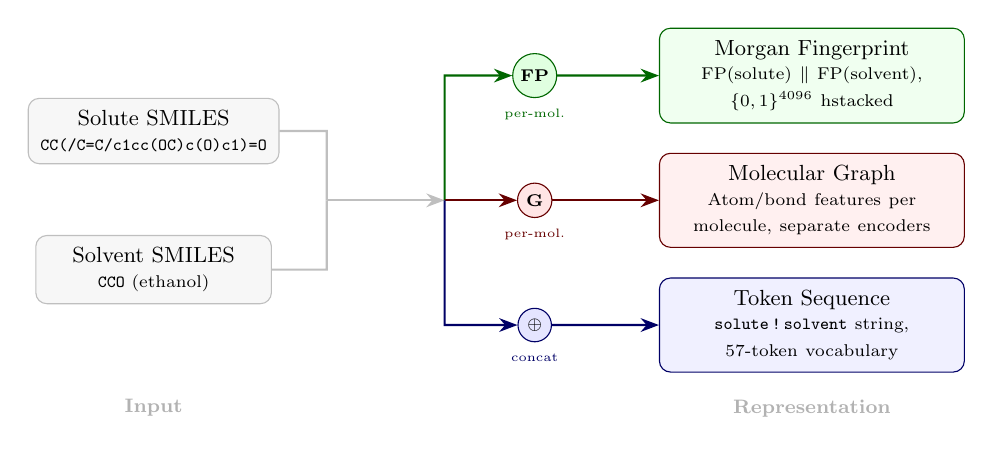
\begin{tikzpicture}[scale=0.88, every node/.style={scale=0.88},
        >=Stealth,
        box/.style={draw, rounded corners=4pt, align=center, font=\small, inner sep=5pt},
        arr/.style={->, thick, draw=gray!50},
    ]
    % ---- Input boxes (identical size) ----
    \node[box, fill=gray!6, draw=gray!50, minimum width=3.4cm] (mol) at (0, 1.0)
        {Solute SMILES\\[-1pt]{\scriptsize\texttt{CC(/C=C/c1cc(OC)c(O)c1)=O}}};
    \node[box, fill=gray!6, draw=gray!50, minimum width=3.4cm] (solv) at (0, -1.0)
        {Solvent SMILES\\[-1pt]{\scriptsize\texttt{CCO} (ethanol)}};

    % ---- Input arrows: two lines join into one arrow ----
    \draw[thick, draw=gray!50] (mol.east) -- (2.5, 1.0) -- (2.5, 0);
    \draw[thick, draw=gray!50] (solv.east) -- (2.5, -1.0) -- (2.5, 0);
    % Single arrow from join point to fork
    \coordinate (fork) at (4.2, 0);
    \draw[arr] (2.5, 0) -- (fork);

    % ---- Green path (top): independent FPs, then hstacked ----
    \node[draw, circle, fill=green!12, draw=green!40!black, inner sep=2pt,
          font=\scriptsize\bfseries] (fpnode) at (5.5, 1.8) {FP};
    \node[font=\tiny, green!40!black, below=1pt of fpnode] {per-mol.};

    \node[box, fill=green!6, draw=green!40!black, minimum width=4.4cm, text width=4.0cm] (fp) at (9.5, 1.8)
        {Morgan Fingerprint\\[-1pt]{\scriptsize FP(solute) $\|$ FP(solvent), $\{0,1\}^{4096}$ hstacked}};

    \draw[arr, draw=green!40!black] (fork) -- (4.2, 1.8) -- (fpnode);
    \draw[arr, draw=green!40!black] (fpnode) -- (fp.west);

    % ---- Red path (middle): molecular graph ----
    \node[draw, circle, fill=red!10, draw=red!40!black, inner sep=2pt,
          font=\scriptsize\bfseries] (graphnode) at (5.5, 0) {G};
    \node[font=\tiny, red!40!black, below=1pt of graphnode] {per-mol.};

    \node[box, fill=red!6, draw=red!40!black, minimum width=4.4cm, text width=4.0cm] (mg) at (9.5, 0)
        {Molecular Graph\\[-1pt]{\scriptsize Atom/bond features per molecule, separate encoders}};

    \draw[arr, draw=red!40!black] (fork) -- (4.2, 0) -- (graphnode);
    \draw[arr, draw=red!40!black] (graphnode) -- (mg.west);

    % ---- Blue path (bottom): SMILES concat, then tokenized ----
    \node[draw, circle, fill=blue!10, draw=blue!40!black, inner sep=2pt,
          font=\scriptsize\bfseries] (cat) at (5.5, -1.8) {$\oplus$};
    \node[font=\tiny, blue!40!black, below=1pt of cat] {concat};

    \node[box, fill=blue!6, draw=blue!40!black, minimum width=4.4cm, text width=4.0cm] (seq) at (9.5, -1.8)
        {Token Sequence\\[-1pt]{\scriptsize \texttt{solute\,!\,solvent} string, 57-token vocabulary}};

    \draw[arr, draw=blue!40!black] (fork) -- (4.2, -1.8) -- (cat);
    \draw[arr, draw=blue!40!black] (cat) -- (seq.west);

    % ---- Stage labels ----
    \node[font=\footnotesize\bfseries, gray!60] at (0, -3.0) {\textsc{Input}};
    \node[font=\footnotesize\bfseries, gray!60] at (9.5, -3.0) {\textsc{Representation}};

    \end{tikzpicture}
    \caption{Input and representation. Both solute and solvent SMILES feed three pathways. The fingerprint path (green) computes Morgan FPs independently per molecule and hstacks them (2048+2048 = 4096-bit). The graph path (red) converts each SMILES to a molecular graph with atom and bond features. The sequence path (blue) concatenates the SMILES strings before tokenization.}
    \label{fig:framework_input}
    \end{subfigure}

    \vspace{0.3cm}

    % ===== (b) Models and Prediction =====
    \begin{subfigure}[b]{\textwidth}
    \centering
    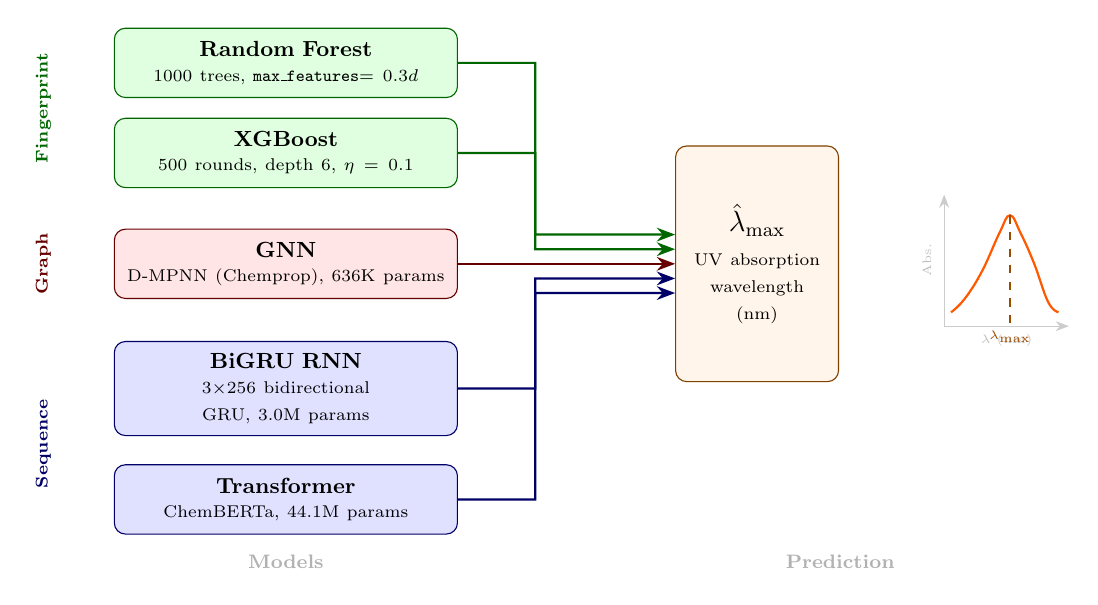
\begin{tikzpicture}[scale=0.88, every node/.style={scale=0.88},
        >=Stealth,
        box/.style={draw, rounded corners=4pt, align=center, font=\small,
                     inner sep=5pt, text width=4.6cm, minimum height=1.0cm},
        arr/.style={->, thick},
    ]

    % ---- Five models, equal spacing, grouped by color ----
    \node[box, fill=green!12, draw=green!40!black] (rf) at (0, 2.9)
        {\textbf{Random Forest}\\[-1pt]{\scriptsize 1000 trees, \texttt{max\_features}$= 0.3d$}};

    \node[box, fill=green!12, draw=green!40!black] (xgb) at (0, 1.6)
        {\textbf{XGBoost}\\[-1pt]{\scriptsize 500 rounds, depth 6, $\eta = 0.1$}};

    \node[box, fill=red!10, draw=red!40!black] (chemprop) at (0, 0)
        {\textbf{GNN}\\[-1pt]{\scriptsize D-MPNN (Chemprop), 636K params}};

    \node[box, fill=blue!12, draw=blue!40!black] (bigru) at (0, -1.8)
        {\textbf{BiGRU RNN}\\[-1pt]{\scriptsize 3$\times$256 bidirectional GRU, 3.0M params}};

    \node[box, fill=blue!12, draw=blue!40!black] (cb) at (0, -3.4)
        {\textbf{Transformer}\\[-1pt]{\scriptsize ChemBERTa, 44.1M params}};

    % ---- Group labels (rotated, centered on each group) ----
    \node[font=\scriptsize\bfseries, green!40!black, rotate=90, anchor=center,
          text width=, minimum height=0pt] at (-3.5, 2.25) {Fingerprint};
    \node[font=\scriptsize\bfseries, red!40!black, rotate=90, anchor=center,
          text width=, minimum height=0pt] at (-3.5, 0) {Graph};
    \node[font=\scriptsize\bfseries, blue!40!black, rotate=90, anchor=center,
          text width=, minimum height=0pt] at (-3.5, -2.6) {Sequence};

    % ---- Output box ----
    \node[box, fill=orange!8, draw=orange!50!black, text width=2.0cm,
          minimum height=3.4cm] (out) at (6.8, 0)
        {\textbf{\large $\hat{\lambda}_{\max}$}\\[3pt]{\scriptsize UV absorption}\\{\scriptsize wavelength (nm)}};

    % ---- Arrows: five models to output ----
    \draw[arr, draw=green!40!black] (rf.east)       -- (3.6, 2.9)   |- ([yshift=12pt]out.west);
    \draw[arr, draw=green!40!black] (xgb.east)      -- (3.6, 1.6)   |- ([yshift=6pt]out.west);
    \draw[arr, draw=red!40!black]   (chemprop.east) -- (3.6, 0)     |- (out.west);
    \draw[arr, draw=blue!40!black]  (bigru.east)    -- (3.6, -1.8)  |- ([yshift=-6pt]out.west);
    \draw[arr, draw=blue!40!black]  (cb.east)       -- (3.6, -3.4)  |- ([yshift=-12pt]out.west);

    % ---- Mini UV spectrum ----
    \begin{scope}[shift={(9.5, 0)}]
        \draw[gray!40, ->] (0,-0.9) -- (0,1.0);
        \node[font=\tiny, gray!50, rotate=90, text width=, minimum height=0pt] at (-0.25, 0.05) {Abs.};
        \draw[gray!40, ->] (0,-0.9) -- (1.8,-0.9);
        \node[font=\tiny, gray!50, text width=, minimum height=0pt] at (0.9, -1.1) {$\lambda$ (nm)};
        \draw[orange!70!red, thick, smooth, tension=0.7]
            plot coordinates {(0.1,-0.7) (0.3,-0.5) (0.55,-0.1) (0.8,0.45) (0.95,0.7) (1.1,0.45) (1.3,0.0) (1.5,-0.55) (1.65,-0.7)};
        \draw[dashed, orange!60!black] (0.95,0.7) -- (0.95,-0.9);
        \node[font=\tiny\bfseries, orange!60!black, text width=, minimum height=0pt] at (0.95, -1.05) {$\lambda_{\max}$};
    \end{scope}

    % ---- Stage labels ----
    \node[font=\footnotesize\bfseries, gray!60, text width=, minimum height=0pt] at (0, -4.3) {\textsc{Models}};
    \node[font=\footnotesize\bfseries, gray!60, text width=, minimum height=0pt] at (8.0, -4.3) {\textsc{Prediction}};

    \end{tikzpicture}
    \caption{Models and prediction. Fingerprint representations feed tree ensembles (green); molecular graphs feed the D-MPNN (red); token sequences feed recurrent and Transformer networks (blue). All five models predict $\lambda_{\max}$.}
    \label{fig:framework_models}
    \end{subfigure}

    \caption{Benchmark framework for UV absorption prediction. (a)~Three representation pathways: Morgan fingerprints computed independently per molecule and horizontally stacked (4096-bit), molecular graphs with atom and bond features, and token sequences formed by SMILES concatenation. (b)~Five models spanning fingerprint, graph, and sequence architectures, all predicting $\lambda_{\max}$.}
    \label{fig:benchmark_framework}
\end{figure}

\FloatBarrier
% ===== Related Work =====
\section{Related Work}
\label{sec:related_work}

Machine learning for UV absorption prediction has evolved from classical QSAR models using handcrafted descriptors to modern deep learning approaches operating on molecular graphs and strings.
We survey the key approaches relevant to our benchmark.

\textbf{Fingerprint-based methods.}
Morgan circular fingerprints~\cite{rogers2010extended}, also known as extended-connectivity fingerprints (ECFP), encode local atomic environments as fixed-length binary vectors and have become the de facto standard molecular representation for classical ML~\cite{wuMoleculeNet2018}.
When combined with tree-based ensemble methods such as Random Forests~\cite{breiman2001random} or gradient boosting~\cite{chen2016xgboost}, fingerprint-based models achieve competitive performance on many molecular property prediction tasks, including aqueous solubility~\cite{delaney2004esol, panapitiya2022evaluation}, toxicity~\cite{mayr2016deeptox}, and UV absorption~\cite{mamede2021machine}.
Mamede et al.~\cite{mamede2021machine} used RF with Morgan fingerprints for ICH~S10~\cite{ICH2013S10} photosafety classification on a 74,784-compound Reaxys dataset, achieving sensitivity 0.90 and specificity 0.88.

\textbf{Sequence models on SMILES.}
The SMILES representation~\cite{weininger1988smiles} maps molecular graphs to character strings, enabling natural language processing techniques for molecular property prediction.
Recurrent neural networks~\cite{elman1990finding}, including Long Short-Term Memory (LSTM)~\cite{hochreiter1997long} and Gated Recurrent Unit (GRU)~\cite{cho2014learning} architectures, process SMILES as sequential data, learning molecular features without explicit descriptor engineering.
Bidirectional variants (BiGRU, BiLSTM)~\cite{schuster1997bidirectional} capture context from both directions, improving representation quality for molecular strings.
Liu et al.\ combined BiGRU with GraphSAGE for molecular toxicity prediction on Tox21~\cite{liuPredictionMolecularToxicity2023}; we adopt only their BiGRU component for SMILES-based regression.
More recently, Transformer architectures~\cite{vaswani2017attention} have been applied to SMILES-based property prediction with attention mechanisms that provide interpretable molecular representations~\cite{hondaSMILESTransformerPretrained2019}.
Chen et al.~\cite{chenMolecularLanguage2023} systematically compared RNNs and Transformers for molecular language modeling, finding that in molecular generation tasks, RNNs better capture local structural features while Transformers excel at global molecular properties and longer sequences.
Although their comparison focused primarily on molecular generation, their conclusion that the optimal architecture depends on the data characteristics may extend to property prediction tasks like UV absorption, where $\lambda_{\max}$ is fundamentally determined by local chromophore features: conjugation length, aromatic character, and heteroatom substituents, as formalized in the classical Woodward--Fieser rules.
This suggests that models encoding local structural information (fingerprints, RNNs) may have an advantage over global-attention architectures for this property, though the extent of this advantage requires empirical validation.
Jiang et al.~\cite{jiang2023trangru} further validated this local/global distinction in their TranGRU architecture, which combines BiGRU for local features with self-attention for global features.
Alternative string representations such as SELFIES~\cite{krenn2020selfies} guarantee chemical validity but have shown mixed results compared to SMILES for property prediction tasks.

\textbf{Graph neural networks.}
GNNs operate directly on molecular graphs through iterative message passing~\cite{gilmer2017neural}, learning atom-level representations from connectivity and atomic features.
Joung et al.~\cite{joung2021deep} reported a Graph Convolutional Neural Network (GCNN) achieving RMSE = 26.6~nm for absorption peak prediction on their Deep4Chem database of 30,094 chromophore--solvent combinations.
Jung et al.~\cite{jung2024machine} compared multiple architectures including a Gradient Boosted Feature Selection (GBFS) pipeline achieving RMSE = 32.2~nm, and a multifidelity approach reaching RMSE = 31.3~nm.
Ghosh et al.~\cite{ghosh2019deep} further showed that neural networks trained on quantum-chemical descriptors can accurately predict excitation spectra, confirming the importance of electronic structure features.

\textbf{Solvent effects.}
Solvatochromism, the shift in absorption wavelength as a function of solvent environment, is a well-studied phenomenon in physical chemistry~\cite{reichardt2011solvents}.
Despite its importance, most ML studies for UV absorption either ignore solvent effects entirely or use categorical solvent labels.
Transfer learning approaches have shown promise for incorporating solvent information in related property prediction tasks~\cite{vermeire2021transfer}\removed{, but systematic evaluation of solvent encoding strategies for UV absorption prediction has been limited}.\added{ The closest prior benchmark of solvent-encoding strategies for UV/Vis absorption is Greenman et al.~\cite{greenman2022multifidelity}, who compared four strategies (no solvent, one-hot solvent labels, Morgan-fingerprint concatenation, and a second D-MPNN encoder for the solvent) within a single multi-fidelity D-MPNN backbone. Their study establishes that explicit solvent representation matters for that backbone and that the dual-encoder multicomponent design is the strongest of the four within-D-MPNN options. Our work occupies the complementary slice of this design space: rather than vary the encoding strategy within one architecture, we fix the strategy at simple concatenation in each architecture's native representation (Morgan-fingerprint concatenation for the tree ensembles, the Chemprop multicomponent dual-encoder for the D-MPNN, and string-level SMILES concatenation for the sequence models) and vary the architecture across five model families. Two of these three native concatenation patterns---SMILES-string concatenation for sequence models, and Morgan-fingerprint concatenation as the model's sole input representation for tree-ensemble regressors---are absent from Greenman et al.'s design grid. The cross-architecture variant lets us test whether the gain from concatenation reflects a model-specific trick or a general principle, and lets us decompose the aggregate benefit into the chromophore-coverage regime where it actually contributes signal (multi-solvent-covered chromophores) versus where it does not (single-solvent or novel chromophores); see the Effect of Solvent Information section and Supporting Information Section~S15.}

\textbf{Benchmarking perspective.}
The MoleculeNet benchmark suite~\cite{wuMoleculeNet2018} established a standardized framework for comparing molecular ML models across diverse property prediction tasks, but UV absorption is not among its benchmarks.
Recent work has highlighted that well-tuned classical models often match or exceed complex architectures~\cite{panapitiya2022evaluation, walters2021applications, fooladi2025evaluating}, challenging the assumption that deep learning always outperforms simpler methods; Fooladi et al.\ benchmarked 14 models across 10 OOD splitting strategies and found that no single architecture dominates across all distribution shifts.
Our study extends this perspective specifically to UV absorption prediction, providing controlled comparisons across three UV absorption datasets with published baselines, complemented by photosafety classification and wetlab validation.


% ===== Methods =====
\section{Methods}
\label{sec:methods}

% --- Dataset Description ---
\subsection{Dataset Description and Preparation}
\label{sec:dataset}

Our primary dataset combines the Joung et al.\ Experimental Database of Optical Properties~\cite{joung2020experimental} and the Beard et al.\ Comparative Dataset of UV/Vis Absorption Spectra~\cite{beard2019comparative}.
\added{A number of other UV absorption / dye datasets exist (Song et al.~\cite{song2025fluortools} survey nine sources in their Table 3, including ChemFluor, SMFluo, ChemDataExtractor, DSSCDB, Fluor-predictor, and Ksenofontov's data). We selected Joung+Beard as the primary dataset for four reasons: (i)~it is the largest unified collection of \emph{purely experimental} solute--solvent $\lambda_{\max}$ measurements available without paywall or license restrictions at the time of submission, with each record carrying an experimental wavelength and an explicit solvent label; (ii)~it has \emph{published baselines} from independent groups (Joung et al.\ GCNN on Deep4Chem~\cite{joung2021deep}, Beard et al.\ DR-CNN, Jung et al.\ multifidelity and GBFS~\cite{jung2024machine}) that enable apples-to-apples comparison without our team training every baseline from scratch; (iii)~combining the two source collections yields broader chromophore coverage than either alone (Deep4Chem 6{,}480 and ChemFluor 4{,}386 unique solutes, vs.\ approximately 7{,}000 in the curated Joung+Beard primary set after our preprocessing); and (iv)~the dataset is dominated by drug-like organic chromophores rather than the dye-aggregation or solar-cell-specific compositions of DSSCDB and Dye-aggregation, matching our intended downstream applications (photosafety screening and wetlab UV-absorber discovery, see Sections~the Photosafety Classification section and the Experimental Validation section).
Among Song's Table 3 entries, several (ChemFluor, SMFluo, Fluor-predictor) measure fluorescence emission rather than UV absorption and are therefore not direct alternatives for our $\lambda_{\max}$ regression task; ChemDataExtractor and Ksenofontov's data provide smaller NLP-extracted or curated subsets that we did not adopt as primary. The Mamede et al.~\cite{mamede2021machine} Reaxys-derived dataset provides binary photosafety labels rather than continuous $\lambda_{\max}$ values, and is used in this work as the basis for the photosafety classification benchmark (the Photosafety Classification section) rather than as a primary regression source.}
Data curation proceeded as follows: (1)~SMILES strings were canonicalized using RDKit~\cite{landrumRdkitRdkit2020_03_12020} to ensure consistent molecular representations; (2)~entries with invalid or unparseable SMILES were removed; (3)~\removed{duplicate records were identified by matching canonical SMILES and solvent identity, retaining the first occurrence}\added{records were grouped by (canonical solute SMILES, canonical solvent SMILES) and the Greenman--Song duplicate-handling protocol~\cite{greenman2022multifidelity,song2025fluortools} was applied: groups whose within-group spread $\max(\lambda_{\max}) - \min(\lambda_{\max}) \leq 5$~nm were collapsed to the mean, and groups whose spread exceeded 5~nm were discarded entirely on the grounds that a within-key disagreement larger than typical instrument resolution likely reflects either a labelling error or a genuinely ambiguous measurement; singletons were retained unchanged}; (4)~solvent names were standardized and mapped to canonical SMILES where possible.\added{ Of the 18{,}755 records that pass dropna and SMILES validation, 18{,}162 were singletons, 253 duplicate groups (508 records) were averaged, and 41 duplicate groups (84 records) were dropped, yielding a cleaned dataset of 18{,}415 unique (solute, solvent) records. We adopt this protocol in preference to the ``retain first occurrence'' rule used in our earlier preprint in response to reviewer feedback (see Supporting Information Section~S9 and the R1-8 entry in the response document).}
After merging\added{ and applying the duplicate-handling protocol}\removed{, deduplication, and canonicalization}, the combined dataset contains \textbf{\removed{18,755}\added{18,415} solute--solvent pairs} spanning \removed{7,016}\added{7,846} unique \removed{chromophores}\added{canonical chromophores} and \removed{365}\added{726 unique canonical} \removed{solvents}\added{solvent SMILES}.\added{ A visual overview of the dataset (the $\lambda_{\max}$ distribution, the top-20 solvent frequencies (log scale), and eight representative chromophore structures spanning the major class diversity) is given in Supporting Information Figure~S1.}

\added{\textbf{Experimental measurement uncertainty.} To contextualise the model errors reported in Table~\ref{tab:model_comparison}, we quantified the inherent measurement noise in the underlying experimental data using two complementary audits (full results in Supporting Information Section~S17). \emph{Within-source} duplicates ((canonical solute, canonical solvent) pairs reported multiple times within the combined v2 dataset before Greenman--Song cleaning) show a heavily right-skewed spread distribution: of $294$ multi-record groups (592 records), the median spread is $0$~nm, $86$\% of groups have spread $\leq 5$~nm, $91$\% are within $20$~nm, and $4.1$\% have spread $> 50$~nm. The Greenman--Song 5-nm cleaning rule (adopted in response to R1-8) therefore retains essentially all duplicates whose spread is consistent with typical UV-Vis instrument precision while discarding the long tail of measurements that disagree by amounts likely attributable to lab-to-lab protocol differences or labelling errors. \emph{Inter-source} disagreement, measured on the $n = 21$ (canonical solute, canonical solvent) pairs reported in both Joung 2020 and Beard 2019, is substantially larger: median $|\Delta\lambda_{\max}| = 49$~nm, RMSD = $48$~nm; note that this small-$n$ sample is dominated by compounds appearing in multiple papers because of solvatochromic interest, which are exactly the chromophores most sensitive to subtle solvent-purity, temperature, or concentration differences across labs. The reported Table~\ref{tab:model_comparison} RMSEs ($31$--$54$~nm) are therefore comparable to the typical $95$th-percentile within-source spread ($21$~nm in Beard alone; $38$~nm in the v2-combined view), and the headline RF$\approx$Chemprop tie may be partially attributable to both architectures operating near the data noise floor on a substantial fraction of test molecules.}
No outlier filtering on $\lambda_{\max}$ values was applied; all experimentally reported values\removed{ in the 200--900~nm range}\added{ (162--1100~nm)} were retained.
Target values ($\lambda_{\max}$) range from \removed{200 to 900}\added{162 to 1100}~nm, with a median of \removed{325}\added{396}~nm\added{; 99.9\% of records lie within 200--900~nm}.

To assess generalizability beyond the primary dataset, we also evaluate on two external datasets using their published split protocols, training models from scratch on each dataset's training split.
The \textbf{Deep4Chem} database~\cite{joung2021deep} contains 30,094 chromophore--solvent combinations; after deduplication and preprocessing, 17,683 records remain (reported GCNN baseline: RMSE = 26.6~nm; 80/10/10 random split). \added{Because Deep4Chem is the source dataset for the Joung half of our primary collection, the two have substantial overlap: 77.4\% of unique Deep4Chem solutes and 72.6\% of its (solute, solvent) pairs also appear in Joung+Beard (overlap analysis in Supporting Information Section~S8 and Figure~S4). Deep4Chem is therefore best characterised as an \emph{in-distribution external} benchmark, useful for reproducing published per-paper baselines under their own splits, but \emph{not} a test of out-of-distribution generalisation.}
The \textbf{Jung et al.\ (2024)} dataset~\cite{jung2024machine} contains approximately 26,000 records with multiple published baselines: GBFS (RMSE = 32.2~nm, MAE = 16.2~nm, $R^2$ = 0.91), Multifidelity (RMSE = 31.3~nm), and DR-CNN (RMSE = 44.4~nm; 72/18/10 random split). \added{Jung 2024 shares 48.8\% of its unique solutes with our primary dataset (about half) and is therefore the more rigorous external test of the two; we use both because the Jung benchmark also exposes us to chromophore families (notably long-wavelength dyes from solar-cell and OLED literature) that are sparsely represented in Joung+Beard.}

\begin{table}[htbp]
\centering
\caption{Summary of the primary Joung+Beard dataset after preprocessing.}
\label{tab:dataset_summary}
\begin{tabular}{lr}
\toprule
\textbf{Attribute} & \textbf{Value} \\
\midrule
Total records \added{(after dedup)} & \removed{18,755}\added{18,415} \\
Unique \added{canonical }chromophores & \removed{7,016}\added{7,846} \\
Unique \added{canonical }solvents & \removed{365}\added{726} \\
$\lambda_{\max}$ range & \removed{200--900}\added{162--1100} nm \\
$\lambda_{\max}$ median & \removed{325}\added{396} nm \\
SMILES vocabulary size & 57 tokens \\
Max sequence length (solute+solvent) & 650 tokens \\
\bottomrule
\end{tabular}
\end{table}


% --- Cross-validation protocol ---
\subsection{Evaluation Protocol}
\label{sec:evaluation}

For the primary dataset, we use \textbf{stratified 5-fold cross-validation}~\cite{kohavi1995study} with a 64/16/20 train/validation/test split.
Stratification is performed on solvent identity (top 20 solvents binned, remainder grouped as ``other'') to ensure representative solvent coverage in each fold, addressing the risk that rare solvents could be absent from test folds.
For deep learning models, the validation set is used exclusively for early stopping (patience = 25 epochs), preventing data leakage from the test set, a methodological concern highlighted in recent benchmarking studies~\cite{panapitiya2022evaluation}.
For fingerprint-based models (RF, XGBoost), training uses only the training fold (validation set unused), ensuring equivalent evaluation conditions.

\added{The 64/16/20 split fractions are not chosen arbitrarily: they arise from a nested-split design in which the outer stratified 5-fold partition (80\% train+val / 20\% test per fold) is composed with an inner solvent-stratified \texttt{train\_test\_split} that carves the trainval portion into 80\% train / 20\% val, yielding 64/16/20 of the total. We note that this stratified-CV protocol does not address the chromophore-overlap concern raised by Greenman et al.~\cite{greenman2022multifidelity}: because the Joung+Beard v3 dataset contains 18{,}415 records but only 7{,}846 unique canonical solutes, each chromophore is on average sampled $\sim$2.3 times under different solvents, and an audit on our 5-fold v3 splits shows that 66.8\% of test records have their solute also appear in the train slice (69.3\% if the val slice is counted) under a different solvent. The full per-model decomposition of test-fold performance into chromophore-seen and chromophore-novel subsets is reported in Supporting Information Section~S10; the headline observation is that all five model families benefit comparably from this overlap (mean $\Delta$RMSE between novel and seen subsets of $+25$ to $+36$~nm), so the RF$\approx$Chemprop tie reported below is not an artefact of the splitting strategy. The Table~\ref{tab:model_comparison} numbers should therefore be interpreted as an upper bound on the architectures' generalisation to novel chromophore scaffolds; the wetlab validation set (the Experimental Validation section) and the lower-overlap Jung 2024 external benchmark (the Cross-Dataset Benchmarking section) provide the more rigorous out-of-distribution picture. We retain the standard stratified-CV protocol for Table~\ref{tab:model_comparison} because it matches the evaluation convention used by Joung, Beard, Greenman, and Jung on these same data, with whose published baselines we want apples-to-apples comparability.}

Metrics are reported as mean $\pm$ standard deviation across five folds: root-mean-square error (RMSE), mean absolute error (MAE), coefficient of determination ($R^2$), and Pearson correlation coefficient ($r$).
Statistical significance of pairwise model differences is assessed using paired $t$-tests across the five fold RMSE values ($\alpha = 0.05$).

For external datasets, we use the exact split protocols published by the original authors to enable direct comparison with reported results.
Our evaluation methodology follows best practices for QSAR/QSPR studies~\cite{tropsha2006best, cherkasov2014qsar}: models are validated using both internal cross-validation and external test sets, multiple statistical metrics are reported, and applicability domain is assessed through out-of-distribution experimental validation (see Experimental Validation).
Models are implemented using scikit-learn~\cite{pedregosa2011scikit} (RF), XGBoost~\cite{chen2016xgboost}, TensorFlow~\cite{abadi2016tensorflow} (BiGRU), Chemprop v2~\cite{yangAnalyzingLearnedMolecular2019} with PyTorch Lightning (D-MPNN), and PyTorch with HuggingFace Transformers~\cite{chithrananda2020chemberta} (pretrained Transformer).
Figure~\ref{fig:model_overview} provides a high-level comparison of the \removed{three}\added{four} model families, illustrating the fundamental differences in molecular representation and model complexity.

% ============== Architecture Overview: 4-panel (R2-6: added D-MPNN panel) ==============

\tikzstyle{archbox} = [rectangle, rounded corners=4pt, minimum width=4cm, minimum height=0.85cm, text centered, draw=black, font=\small]
\tikzstyle{archboxnarrow} = [rectangle, rounded corners=4pt, minimum width=3.0cm, minimum height=0.85cm, align=center, draw=black, font=\small]
\tikzstyle{archarrow} = [thick,-{Stealth[length=2.5mm]}]

\begin{figure}[htbp]
\centering

% ---- (a) RANDOM FOREST ----
\begin{minipage}[t]{0.23\textwidth}
\centering
\begin{tikzpicture}[node distance=1.35cm, scale=0.78, transform shape, baseline=(current bounding box.north)]
\node (smi)   [archboxnarrow, fill=gray!15]                     {SMILES Input};
\node (fp)    [archboxnarrow, fill=green!12, below of=smi]      {Morgan FP ($r{=}2$)};
\node (vec)   [archboxnarrow, fill=green!20, below of=fp]       {2048-bit vector};
\node (trees) [archboxnarrow, fill=green!30, below of=vec]      {1000 Decision Trees};
\node (avg)   [archboxnarrow, fill=green!15, below of=trees]    {Ensemble Average};
\node (out)   [archboxnarrow, fill=red!12, below of=avg]        {$\hat{\lambda}_{\max}$};

\draw [archarrow] (smi)   -- (fp);
\draw [archarrow] (fp)    -- (vec);
\draw [archarrow] (vec)   -- (trees);
\draw [archarrow] (trees) -- (avg);
\draw [archarrow] (avg)   -- (out);

% Invisible spacers to match height of taller panels — 3 extra nodes
\node[below of=out, minimum width=3.0cm, minimum height=0.85cm] (sp1) {};
\node[below of=sp1, minimum width=3.0cm, minimum height=0.85cm] (sp2) {};
\node[below of=sp2, minimum width=3.0cm, minimum height=0.85cm] (sp3) {};
\end{tikzpicture}

\textbf{(a)} Random Forest\\[2pt]
{\scriptsize No GPU, $\sim$15 min total}
\end{minipage}
\hfill
% ---- (b) D-MPNN (Chemprop) -- NEW PANEL added per R2-6 ----
\begin{minipage}[t]{0.23\textwidth}
\centering
\begin{tikzpicture}[node distance=1.35cm, scale=0.78, transform shape, baseline=(current bounding box.north)]
\node (smi)  [archboxnarrow, fill=gray!15]                      {Solute + Solvent\\SMILES};
\node (grp)  [archboxnarrow, fill=cyan!10, below of=smi]        {RDKit $\to$ graphs};
\node (mp1)  [archboxnarrow, fill=cyan!20, below of=grp]        {Solute D-MPNN\\($T{=}3$, $d_h{=}300$)};
\node (mp2)  [archboxnarrow, fill=cyan!20, below of=mp1]        {Solvent D-MPNN\\($T{=}3$, $d_h{=}300$)};
\node (pool) [archboxnarrow, fill=cyan!30, below of=mp2]        {Mean-pool $\oplus$ concat};
\node (ffn)  [archboxnarrow, fill=purple!12, below of=pool]     {FFN (300, ReLU)};
\node (head) [archboxnarrow, fill=purple!15, below of=ffn]      {Linear head};
\node (out)  [archboxnarrow, fill=red!12, below of=head]        {$\hat{\lambda}_{\max}$};

\draw [archarrow] (smi)  -- (grp);
\draw [archarrow] (grp)  -- (mp1);
\draw [archarrow] (mp1)  -- (mp2);
\draw [archarrow] (mp2)  -- (pool);
\draw [archarrow] (pool) -- (ffn);
\draw [archarrow] (ffn)  -- (head);
\draw [archarrow] (head) -- (out);

\node[below of=out, minimum width=3.0cm, minimum height=0.85cm] (sp1) {};
\end{tikzpicture}

\textbf{(b)} D-MPNN (Chemprop)\\[2pt]
{\scriptsize 636K params, $\sim$1.5 hr/fold}
\end{minipage}
\hfill
% ---- (c) BiGRU (optimized) ----
\begin{minipage}[t]{0.23\textwidth}
\centering
\begin{tikzpicture}[node distance=1.35cm, scale=0.78, transform shape, baseline=(current bounding box.north)]
\node (smi)  [archboxnarrow, fill=gray!15]                     {SMILES Input};
\node (tok)  [archboxnarrow, fill=teal!10, below of=smi]       {Char Tokenization};
\node (emb)  [archboxnarrow, fill=teal!20, below of=tok]       {Embedding ($d{=}50$)};
\node (gru1) [archboxnarrow, fill=teal!30, below of=emb]       {BiGRU L1 (256$\times$2)};
\node (gru2) [archboxnarrow, fill=teal!30, below of=gru1]      {BiGRU L2 (256$\times$2)};
\node (gru3) [archboxnarrow, fill=teal!30, below of=gru2]      {BiGRU L3 (256$\times$2)};
\node (den)  [archboxnarrow, fill=purple!12, below of=gru3]    {Dense (128, ReLU)};
\node (drop) [archboxnarrow, fill=orange!10, below of=den]     {Dropout (0.105)};
\node (out)  [archboxnarrow, fill=red!12, below of=drop]       {$\hat{\lambda}_{\max}$};

\draw [archarrow] (smi)  -- (tok);
\draw [archarrow] (tok)  -- (emb);
\draw [archarrow] (emb)  -- (gru1);
\draw [archarrow] (gru1) -- (gru2);
\draw [archarrow] (gru2) -- (gru3);
\draw [archarrow] (gru3) -- (den);
\draw [archarrow] (den)  -- (drop);
\draw [archarrow] (drop) -- (out);
\end{tikzpicture}

\textbf{(\removed{b}\added{c})} BiGRU (optimized)\\[2pt]
{\scriptsize 3.0M params, $\sim$5 hr/fold}
\end{minipage}
\hfill
% ---- (d) ChemBERTa ----
\begin{minipage}[t]{0.23\textwidth}
\centering
\begin{tikzpicture}[node distance=1.35cm, scale=0.78, transform shape, baseline=(current bounding box.north)]
\node (smi)  [archboxnarrow, fill=gray!15]                      {SMILES Input};
\node (tok)  [archboxnarrow, fill=violet!10, below of=smi]      {BPE Tokenization};
\node (pre)  [archboxnarrow, fill=violet!18, below of=tok]      {Pretrained (ZINC)};
\node (trn1) [archboxnarrow, fill=violet!28, below of=pre]      {Transformer Layer 1};
\node (trn2) [archboxnarrow, fill=violet!28, below of=trn1]     {$\vdots$ (6 layers total)};
\node (trn6) [archboxnarrow, fill=violet!28, below of=trn2]     {Transformer Layer 6};
\node (cls)  [archboxnarrow, fill=violet!12, below of=trn6]     {{[CLS]} Pooling};
\node (head) [archboxnarrow, fill=purple!15, below of=cls]      {Regression Head};
\node (out)  [archboxnarrow, fill=red!12, below of=head]        {$\hat{\lambda}_{\max}$};

\draw [archarrow] (smi)  -- (tok);
\draw [archarrow] (tok)  -- (pre);
\draw [archarrow] (pre)  -- (trn1);
\draw [archarrow] (trn1) -- (trn2);
\draw [archarrow] (trn2) -- (trn6);
\draw [archarrow] (trn6) -- (cls);
\draw [archarrow] (cls)  -- (head);
\draw [archarrow] (head) -- (out);
\end{tikzpicture}

\textbf{(\removed{c}\added{d})} ChemBERTa\\[2pt]
{\scriptsize 44.1M params, $\sim$3 hr/fold}
\end{minipage}

\caption{Architecture comparison of the \removed{three}\added{four} model families \added{benchmarked in this work}. (a)~Random Forest operates on precomputed 2048-bit Morgan fingerprints; an ensemble of 1000 trees votes on $\lambda_{\max}$, requiring no GPU. \added{(b)~Chemprop D-MPNN uses two parallel directed message-passing encoders (one for the solute molecular graph and one for the solvent) and concatenates their mean-pooled representations before a feed-forward regression head; 636K parameters at default hyperparameters.} (\removed{b}\added{c})~BiGRU (optimized via Bayesian HPO) processes character-level SMILES through 3 stacked bidirectional GRU layers with 256 units per direction. (\removed{c}\added{d})~ChemBERTa fine-tunes a 6-layer Transformer (12 attention heads, 768 hidden dim) pretrained on SMILES from the ZINC database; the \texttt{[CLS]} representation is passed to a regression head. \removed{All models receive solvent information via SMILES concatenation.}\added{Solvent information is conveyed by SMILES concatenation in (a, c, d) and by the parallel-encoder multicomponent configuration in (b). XGBoost (not shown) shares (a)'s pipeline with a gradient-boosted tree ensemble in place of the RF.}}
\label{fig:model_overview}
\end{figure}


\FloatBarrier
% --- Model Architectures ---
\subsection{Random Forest with Morgan Fingerprints}
\label{sec:rf}

\removed{Random Forest (RF)~\cite{breiman2001random} is an ensemble method that constructs $B$ decision trees, each trained on a bootstrap sample of the data, and averages their predictions to reduce variance.
For a regression task, the ensemble prediction is:
\begin{equation}
    \hat{y}(\vect{x}) = \frac{1}{B} \sum_{b=1}^{B} T_b(\vect{x})
\end{equation}
where $T_b$ denotes the $b$-th decision tree.
Each tree partitions the feature space by recursively selecting the feature $j$ and threshold $s$ that minimize the mean squared error (MSE) within each resulting partition:
\begin{equation}
    (j^*, s^*) = \arg\min_{j, s} \left[ \sum_{x_i \in R_1(j,s)} (y_i - \bar{y}_{R_1})^2 + \sum_{x_i \in R_2(j,s)} (y_i - \bar{y}_{R_2})^2 \right]
\end{equation}
where $R_1$ and $R_2$ are the two regions defined by the split and $\bar{y}_{R_k}$ is the mean target in region $R_k$.
At each split, only a random subset of features (out of $d$ total) is considered, decorrelating the trees and improving generalization.

The input representation for RF is the Morgan circular fingerprint~\cite{rogers2010extended}, which encodes local chemical environments by enumerating all atom-centered circular substructures up to a specified radius $r$.
Each substructure is hashed to a fixed-length binary vector of $n$ bits:
\begin{equation}
    \vect{x} = \text{MorganFP}(\text{mol}, r=2, n=2048) \in \{0, 1\}^{2048}
\end{equation}
Hyperparameters were selected via grid search over 432 configurations (varying $B$, max depth, min leaf size, features per split, FP radius, and FP length) evaluated on a held-out validation fold.
The optimal configuration uses $B = 1000$ trees, no maximum depth constraint, and $\lfloor 0.3d \rfloor$ features considered per split (scikit-learn \texttt{RandomForestRegressor}).}

\added{Random Forest (RF)~\cite{breiman2001random} is an ensemble of decision trees averaging predictions over bootstrap-sampled subsets, with random feature subsetting at each split to decorrelate the trees. We use scikit-learn's \texttt{RandomForestRegressor} with hyperparameters selected via grid search over 432 configurations: $n_\text{trees} = 1000$, $\text{max\_features} = 0.3$, $\text{min\_samples\_leaf} = 1$, no maximum depth constraint (full RF hyperparameter sensitivity analysis in Supporting Information Section~S3). The input representation is a Morgan circular fingerprint~\cite{rogers2010extended} of radius 2 and length 2048 computed separately for the solute and the solvent and concatenated into a 4096-bit feature vector (the Solvent Information Encoding section). The full mathematical formulation of the ensemble estimator, the MSE-minimising split criterion, and the Morgan fingerprint hashing is given in Supporting Information Section~S12.}


\subsection{Gradient Boosting (XGBoost)}
\label{sec:xgboost}

\removed{XGBoost~\cite{chen2016xgboost} constructs an additive ensemble of decision trees trained sequentially, where each new tree $f_t$ fits the residual errors of the current ensemble.
The prediction after $T$ boosting rounds is:
\begin{equation}
    \hat{y}(\vect{x}) = \sum_{t=1}^{T} \eta \cdot f_t(\vect{x})
\end{equation}
where $\eta$ is the learning rate (shrinkage parameter) that controls the contribution of each tree.
Each tree $f_t$ is trained to minimize a regularized objective combining the loss on residuals and a penalty on tree complexity:
\begin{equation}
    \mathcal{L}^{(t)} = \sum_{i=1}^{n} l\!\left(y_i,\; \hat{y}_i^{(t-1)} + f_t(\vect{x}_i)\right) + \Omega(f_t)
\end{equation}
where $\Omega(f_t) = \gamma \cdot |\text{leaves}| + \tfrac{1}{2}\lambda \sum_j w_j^2$ penalizes the number of leaves and the magnitude of leaf weights $w_j$.
We use $T = 500$ rounds, max depth 6, $\eta = 0.1$, and histogram-based tree construction.
The same Morgan fingerprint input (concatenated solute + solvent, 4096 bits total) is used as for RF.}

\added{XGBoost~\cite{chen2016xgboost} is a gradient-boosted decision-tree ensemble trained to sequentially fit residual errors of the running prediction, with a regularised objective that penalises both the number of leaves and the magnitude of leaf weights. We use $T = 500$ boosting rounds, max depth 6, learning rate $\eta = 0.1$, and histogram-based tree construction on the same 4096-bit Morgan fingerprint input as RF. Full boosting prediction formula and regularised objective in Supporting Information Section~S12.}


\subsection{Recurrent Neural Networks and BiGRU}
\label{sec:bigru}

\removed{Recurrent neural networks (RNNs)~\cite{elman1990finding} process sequential input by maintaining a hidden state $\vect{h}_t$ that is updated at each time step $t$:
\begin{equation}
    \vect{h}_t = \sigma(\matr{W}_h \vect{h}_{t-1} + \matr{W}_x \vect{x}_t + \vect{b})
\end{equation}
where $\vect{x}_t$ is the input at step $t$, $\matr{W}_h$ and $\matr{W}_x$ are weight matrices, and $\sigma$ is a nonlinear activation.
Standard RNNs suffer from vanishing gradients over long sequences, motivating gated architectures.

The Gated Recurrent Unit (GRU)~\cite{cho2014learning} addresses this through two gating mechanisms, an update gate $\vect{z}_t$ and a reset gate $\vect{r}_t$, that control information flow:
\begin{align}
    \vect{z}_t &= \sigma(\matr{W}_z \vect{x}_t + \matr{U}_z \vect{h}_{t-1} + \vect{b}_z) \label{eq:gru_update} \\
    \vect{r}_t &= \sigma(\matr{W}_r \vect{x}_t + \matr{U}_r \vect{h}_{t-1} + \vect{b}_r) \label{eq:gru_reset} \\
    \tilde{\vect{h}}_t &= \tanh(\matr{W}_h \vect{x}_t + \matr{U}_h (\vect{r}_t \odot \vect{h}_{t-1}) + \vect{b}_h) \label{eq:gru_candidate} \\
    \vect{h}_t &= (1 - \vect{z}_t) \odot \vect{h}_{t-1} + \vect{z}_t \odot \tilde{\vect{h}}_t \label{eq:gru_output}
\end{align}
where $\sigma$ is the sigmoid function and $\odot$ denotes element-wise multiplication.
The update gate $\vect{z}_t$ determines how much of the previous state to retain versus replace with the candidate $\tilde{\vect{h}}_t$, while the reset gate $\vect{r}_t$ controls how much past information is used to compute the candidate.
This gating mechanism enables GRUs to capture long-range dependencies without the vanishing gradient problem.

A Bidirectional GRU (BiGRU)~\cite{schuster1997bidirectional} processes the sequence in both directions, concatenating the forward and backward hidden states to capture context from both ends of the molecular string:
\begin{equation}
    \vect{h}_t^{\text{bi}} = [\overrightarrow{\vect{h}_t} \| \overleftarrow{\vect{h}_t}]
\end{equation}

Our BiGRU model operates on character-level tokenized SMILES using a 57-token vocabulary.
An embedding layer maps each token to a 50-dimensional dense vector, followed by two stacked BiGRU layers (128 units per direction), a dense layer (128 units, ReLU), dropout (0.2), and a linear output.
The model has approximately 470K trainable parameters and is trained with RMSprop (lr = 0.001), MAE loss, batch size 32, for up to 250 epochs with early stopping on validation MAE (patience 25).
Mixed-precision (float16) training is used on an NVIDIA RTX 4090 GPU.
This architecture is inspired by the BiGRU component of Liu et al.~\cite{liuPredictionMolecularToxicity2023}, who combined BiGRU with GraphSAGE for SMILES-based molecular toxicity prediction on the Tox21 dataset; we use only the BiGRU branch for regression.}

\added{The Bidirectional Gated Recurrent Unit (BiGRU)~\cite{schuster1997bidirectional,cho2014learning} processes a SMILES sequence in both forward and backward directions and concatenates the per-step hidden states to produce a context-aware representation at each token; the architecture in this work is inspired by the BiGRU component of Liu et al.~\cite{liuPredictionMolecularToxicity2023}, who combined a BiGRU branch with a GraphSAGE branch for SMILES-based molecular toxicity prediction on Tox21, we use only the BiGRU branch for regression. Our default model operates on a 57-token character-level SMILES vocabulary with a 50-dimensional embedding, two stacked BiGRU layers (128 units per direction), a 128-unit dense layer with ReLU, dropout 0.2, and a linear scalar output ($\sim$470K trainable parameters). Training uses RMSprop (lr $= 10^{-3}$), MAE loss, batch size 32, mixed-precision (float16) on an NVIDIA RTX 4090 GPU, with up to 250 epochs and early stopping on validation MAE (patience 25). Full vanilla-RNN update, GRU gating equations (update, reset, candidate, output gates), and the BiGRU forward/backward concatenation are given in Supporting Information Section~S12.}

To address the asymmetric tuning concern, we also perform Bayesian hyperparameter optimization (HPO) using Optuna~\cite{akiba2019optuna} with the Tree-structured Parzen Estimator (TPE) sampler.
The search space covers the number of BiGRU units per direction $\in \{64, 128, 256\}$, number of stacked BiGRU layers $\in \{1, 2, 3\}$, embedding dimension $\in \{32, 50, 100\}$, dropout rate $\in [0.1, 0.4]$, learning rate $\in [10^{-4}, 3 \times 10^{-3}]$, and batch size $\in \{32, 64, 128\}$.
Each trial trains on the fold~0 training set with early stopping on the fold~0 validation set (MAE loss, patience 25).
After 25 trials, the best configuration (256 units per direction, 3 stacked BiGRU layers with $\sim$2.97M parameters, embedding dimension 50, dropout 0.105, learning rate $1.1 \times 10^{-3}$, batch size 128) achieves a fold-0 validation RMSE of 33.33~nm; full 5-fold cross-validation \removed{yields RMSE = $34.71 \pm 1.40$~nm, a 4.8\% improvement over the default 36.45~nm}\added{on the v3 deduplicated primary dataset yields RMSE = $36.20 \pm 1.20$~nm, comparable to the 34.71~nm obtained on the earlier first-occurrence-dedup data and consistent with the broader $\sim$1.5~nm BiGRU drift we observe between v2 and v3 (see Supporting Information Section~S9)}.
Key findings from the HPO landscape: (1) three-layer architectures consistently outperform two-layer defaults, (2) single-layer models fail entirely (validation RMSE $>$44~nm), (3) low dropout ($\sim$0.10) is optimal for the larger architecture, and (4) embedding dimension 50 outperforms both 32 and 100.
Full cross-validated results with this tuned architecture are reported in the Results section.
Figure~\ref{fig:bigru_architectures} compares the default and optimized BiGRU architectures.

\tikzstyle{layerbox} = [rectangle, rounded corners=3pt, minimum width=4.2cm, minimum height=0.8cm, text centered, draw=black, font=\small]
\tikzstyle{layerarrow} = [thick,->,>=stealth]

\begin{figure}[htbp]
\centering

\begin{minipage}[t]{0.45\textwidth}
\centering
\begin{tikzpicture}[node distance=1.3cm, scale=0.82, transform shape, baseline=(current bounding box.north)]
\node (emb)  [layerbox, fill=blue!15]                    {Embedding ($d=50$)};
\node (gru1) [layerbox, fill=green!20, below of=emb]     {BiGRU Layer 1 (128$\times$2)};
\node (gru2) [layerbox, fill=green!20, below of=gru1]    {BiGRU Layer 2 (128$\times$2)};
\node (den)  [layerbox, fill=purple!15, below of=gru2]   {Dense (128, ReLU)};
\node (drop) [layerbox, fill=orange!15, below of=den]    {Dropout (0.20)};
\node (out)  [layerbox, fill=red!15, below of=drop]      {Linear Output $\rightarrow$ 1};
\draw [layerarrow] (emb)  -- (gru1);
\draw [layerarrow] (gru1) -- (gru2);
\draw [layerarrow] (gru2) -- (den);
\draw [layerarrow] (den)  -- (drop);
\draw [layerarrow] (drop) -- (out);
\node[font=\scriptsize, gray, right] at (2.4, 0)     {$T \times 50$};
\node[font=\scriptsize, gray, right] at (2.4, -1.3)  {$T \times 256$};
\node[font=\scriptsize, gray, right] at (2.4, -2.6)  {$256$};
\node[font=\scriptsize, gray, right] at (2.4, -3.9)  {$128$};
\node[font=\scriptsize, gray, right] at (2.4, -5.2)  {$128$};
\node[font=\scriptsize, gray, right] at (2.4, -6.5)  {$1$};
% Invisible spacer to match height of (b)
\node[below=1.3cm of out] (spacer) {};
\end{tikzpicture}

\textbf{(a)} Default BiGRU\\[2pt]
{\small 2 layers, 128 units, $\sim$470K params\\Inspired by Liu et al.\ (2023)}
\end{minipage}
\hfill
\begin{minipage}[t]{0.45\textwidth}
\centering
\begin{tikzpicture}[node distance=1.3cm, scale=0.82, transform shape, baseline=(current bounding box.north)]
\node (emb)  [layerbox, fill=blue!15]                    {Embedding ($d=50$)};
\node (gru1) [layerbox, fill=green!35, below of=emb]     {BiGRU Layer 1 (256$\times$2)};
\node (gru2) [layerbox, fill=green!35, below of=gru1]    {BiGRU Layer 2 (256$\times$2)};
\node (gru3) [layerbox, fill=green!35, below of=gru2]    {BiGRU Layer 3 (256$\times$2)};
\node (den)  [layerbox, fill=purple!15, below of=gru3]   {Dense (128, ReLU)};
\node (drop) [layerbox, fill=orange!15, below of=den]    {Dropout (0.105)};
\node (out)  [layerbox, fill=red!15, below of=drop]      {Linear Output $\rightarrow$ 1};
\draw [layerarrow] (emb)  -- (gru1);
\draw [layerarrow] (gru1) -- (gru2);
\draw [layerarrow] (gru2) -- (gru3);
\draw [layerarrow] (gru3) -- (den);
\draw [layerarrow] (den)  -- (drop);
\draw [layerarrow] (drop) -- (out);
\node[font=\scriptsize, gray, right] at (2.4, 0)     {$T \times 50$};
\node[font=\scriptsize, gray, right] at (2.4, -1.3)  {$T \times 512$};
\node[font=\scriptsize, gray, right] at (2.4, -2.6)  {$T \times 512$};
\node[font=\scriptsize, gray, right] at (2.4, -3.9)  {$512$};
\node[font=\scriptsize, gray, right] at (2.4, -5.2)  {$128$};
\node[font=\scriptsize, gray, right] at (2.4, -6.5)  {$128$};
\node[font=\scriptsize, gray, right] at (2.4, -7.8)  {$1$};
\end{tikzpicture}

\textbf{(b)} Optimized BiGRU\\[2pt]
{\small 3 layers, 256 units, $\sim$3.0M params\\Optuna HPO (25 trials, 4.8\% $\downarrow$ RMSE)}
\end{minipage}

\caption{BiGRU architecture comparison. (a)~Default architecture inspired by Liu et al.~\cite{liuPredictionMolecularToxicity2023}: 2 stacked BiGRU layers with 128 units per direction. (b)~Optimized architecture from Bayesian HPO: 3 stacked BiGRU layers with 256 units per direction, lower dropout, yielding 6.3$\times$ more parameters and 4.8\% lower cross-validated RMSE. Both share the same embedding dimension ($d=50$) and training procedure (RMSprop, MAE loss, early stopping).}
\label{fig:bigru_architectures}
\end{figure}


\FloatBarrier
\subsection{Pretrained Transformer}
\label{sec:chemberta}

To assess whether pretraining on large molecular corpora bridges the gap between sequence models and fingerprint-based approaches, we adopt ChemBERTa~\cite{chithrananda2020chemberta} as our Transformer representative.
ChemBERTa is a RoBERTa~\cite{liu2019roberta} architecture pretrained on SMILES from the ZINC database~\cite{irwin2005zinc}, selected because it is among the most widely used pretrained molecular Transformers and provides a direct comparison between pretrained global-attention and locally biased architectures.
It uses a byte-pair encoding (BPE) tokenizer trained on SMILES, with 6 Transformer layers, 12 attention heads, and a hidden dimension of 768, totaling 44.1M parameters.

We fine-tune ChemBERTa for regression by adding a linear prediction head (768 $\to$ 256 $\to$ 1) on top of the \texttt{[CLS]} token representation.
Solvent information is encoded by concatenating solute and solvent SMILES with a dot separator (\texttt{solute.solvent}), analogous to the exclamation-mark separator used for BiGRU.
Fine-tuning uses AdamW~\cite{loshchilov2019decoupled} with learning rate $5 \times 10^{-5}$, weight decay 0.01, linear warmup (200 steps) followed by linear decay, Huber loss ($\beta = 10$), batch size 32, and early stopping on validation MAE (patience 15 epochs, maximum 100 epochs).
Mixed-precision (float16) training is used on the same NVIDIA RTX 4090 GPU.


\subsection{Graph Neural Network (D-MPNN)}
\label{sec:chemprop}

\removed{To include a 2D graph-based representation, we adopt the Directed Message Passing Neural Network (D-MPNN) architecture via Chemprop~\cite{yangAnalyzingLearnedMolecular2019}, selected for its established performance across diverse molecular property benchmarks and its native support for multicomponent (solute--solvent) inputs.
The D-MPNN operates on the molecular graph by passing messages along directed bonds rather than atoms, avoiding redundant information flow to the source atom at each step.
Given a molecular graph with atom features $\vect{x}_v$ and bond features $\vect{e}_{vw}$, directed bond hidden states $\vect{h}_{vw}^{(t)}$ are updated over $T$ steps:
\begin{equation}
    \vect{h}_{vw}^{(t)} = \tau\!\left(\vect{h}_{vw}^{(0)} + \matr{W}_t \sum_{u \in N(v) \setminus w} \vect{h}_{uv}^{(t-1)}\right)
\end{equation}
where $\tau$ is ReLU, $N(v) \setminus w$ denotes neighbors of $v$ excluding $w$, and $\vect{h}_{vw}^{(0)} = \tau(\matr{W}_0 \, [\vect{x}_v \| \vect{e}_{vw}])$ is initialized from concatenated atom and bond features.
After $T = 3$ message-passing steps, atom-level representations are obtained by summing incoming bond messages and passed through mean pooling to produce a fixed-length molecular vector.

We adapt the D-MPNN for solute--solvent prediction using a multicomponent configuration: separate D-MPNN encoders process the solute and solvent molecular graphs independently (hidden dimension $d_h = 300$ each), and their pooled representations are concatenated before a feed-forward regression head.
All D-MPNN hyperparameters are kept at their published defaults~\cite{yangAnalyzingLearnedMolecular2019}; no architecture or hyperparameter tuning was performed.
This yields 636K trainable parameters.
Target values are normalized to zero mean and unit variance during training.
We use the Noam learning rate schedule (warmup from $10^{-4}$ to $10^{-3}$ over 2 epochs, then exponential decay to $10^{-4}$), batch size 64, and early stopping on validation loss (patience 15, maximum 100 epochs).}

\added{The Directed Message Passing Neural Network (D-MPNN) implemented in Chemprop v2~\cite{yangAnalyzingLearnedMolecular2019,chempropv2_2024} operates on the molecular graph by passing messages along directed bonds (rather than atoms), avoiding redundant information flow to the source atom at each step. We use Chemprop's built-in multicomponent configuration for solute--solvent prediction: separate D-MPNN encoders process the solute and solvent molecular graphs independently (hidden dimension $d_h = 300$ each, $T = 3$ message-passing steps, mean-pool readout), and their pooled representations are concatenated before a feed-forward regression head. The default D-MPNN hyperparameters are taken from Chemprop's published v2 release~\cite{yangAnalyzingLearnedMolecular2019,chempropv2_2024}, yielding 636K trainable parameters; in response to reviewer concern R1-12 we also ran a 25-trial Optuna probe of Chemprop's hyperparameters (matching the budget used for BiGRU), which improves cross-validated RMSE from $33.15 \pm 3.27$ to $28.83 \pm 1.32$~nm by primarily eliminating fold-4's early-stopping outlier in the default run (full search space and per-fold comparison in Supporting Information Section~S13). The tuned configuration is reported as a separate row in Table~\ref{tab:model_comparison}; we retain the default configuration as the primary Table~\ref{tab:model_comparison} comparison to match the evaluation convention used by published Chemprop benchmarks on these data~\cite{joung2021deep,beard2019comparative,greenman2022multifidelity,jung2024machine,chempropv2_2024}, and the tuned vs.\ RF advantage is borderline at $n = 5$ folds (parametric paired $t$-test $p = 0.044$, Wilcoxon $p = 0.125$). Target values are normalised to zero mean and unit variance during training. We use the Noam learning-rate schedule (warmup from $10^{-4}$ to $10^{-3}$ over 2 epochs, then exponential decay to $10^{-4}$), batch size 64, and early stopping on validation loss (patience 15, maximum 100 epochs). With $\sim$11{,}780 training records per fold (the 64\% train portion of the v3 dataset), the default configuration corresponds to a parameter-to-sample ratio of $\sim$54 parameters per training example, higher than the $\sim$10--20 typical of from-scratch QSPR models but well below the $\geq 10^3$ characteristic of pretrained transfer-learning regimes. The Chemprop v2 release paper~\cite{chempropv2_2024} validates this regime across moderate-size molecular property datasets and relies on three regularisation mechanisms in lieu of explicit parameter reduction: the Noam learning-rate decay (which limits effective gradient magnitude in late training), early stopping on val loss with patience 15 (which truncates training as soon as overfitting begins), and a default dropout of $0.0$ in the message-passing and FFN heads (deliberately disabled because Chemprop's authors found target-normalisation plus early stopping sufficient on the datasets it was tuned for). The R1-12 HPO probe confirms that adding a modest $0.1$ dropout improves cross-validated RMSE by $\sim$4~nm and reduces fold variance (Section~S13), so the published defaults are conservative but not pathological at this dataset size. Full message-passing recurrence and the initialisation of bond hidden states from concatenated atom and bond features in Supporting Information Section~S12.}


% --- Solvent Concatenation ---
\subsection{Solvent Information Encoding}
\label{sec:solvent}

UV absorption wavelengths are solvent-dependent properties: the same chromophore can exhibit different $\lambda_{\max}$ values in different solvents (solvatochromism)~\cite{reichardt2011solvents}.\added{ An empirical audit of the v3 dataset quantifies the size of this effect: of the $7{,}846$ unique chromophores, $2{,}516$ ($32$\%) appear under $\geq 2$ canonical solvents in the v3 cleaning; for these, the per-chromophore span $\max(\lambda_{\max}) - \min(\lambda_{\max})$ has median $10$~nm and $95$th percentile $52$~nm, with a long tail extending to $> 200$~nm for the strongest solvatochromic compounds in the dataset. The top-decile chromophores by span are dominated by classical solvatochromism standards (Reichardt's $E_T(30)$ dye reaches a $494$~nm span across $334$ different solvents in the dataset) and push--pull merocyanines / stilbene-pyridinium cyanines whose intramolecular charge transfer is strongly stabilised in polar solvents (full per-chromophore distribution and top-15 table in Supporting Information Section~S18).}
We encode solvent information by concatenating the solute and solvent SMILES into a single input string:
\begin{equation}
    S_{\text{input}} = \texttt{!} \oplus S_{\text{solute}} \oplus \texttt{!} \oplus S_{\text{solvent}} \oplus \texttt{E}
\end{equation}
where \texttt{!} serves as the start/separator token and \texttt{E} as the end/padding token.

For fingerprint-based models, we adopt an analogous strategy: Morgan fingerprints are computed separately for the solute and solvent, then concatenated into a single feature vector (2048 + 2048 = 4096 dimensions).
This ``solvent concatenation'' approach requires no domain-specific descriptor engineering and enables both model families to learn solvent effects from molecular structure alone.


% ===== Results and Discussion =====
\section{Results and Discussion}
\label{sec:results}

% --- Model Comparison ---
\subsection{Model Comparison on Joung+Beard Dataset}
\label{sec:model_comparison}

Table~\ref{tab:model_comparison} presents the performance of all models on the primary dataset using stratified 5-fold cross-validation with proper train/validation/test separation.

\begin{table}[htbp]
\centering
\caption{\removed{Model comparison on the Joung+Beard dataset (18,755 samples, stratified 5-fold CV, 64/16/20 train/val/test split). Best values in bold. $\pm$ denotes standard deviation across folds.}\added{Model comparison on the Joung+Beard dataset (18,415 samples after Greenman--Song duplicate handling, stratified 5-fold CV, 64/16/20 train/val/test split). Best values in bold. $\pm$ denotes standard deviation across folds. All five model families were re-trained on the v3 cleaned dataset; cross-validated mean RMSE shifted by $\leq$1.5~nm for the four local-feature models and by 3.7~nm for ChemBERTa, with the qualitative ranking and the RF$\approx$Chemprop tie preserved (see Supporting Information Section~S9 for the v2-vs-v3 comparison table).}}
\label{tab:model_comparison}
\added{%
\begin{tabular}{lcccc}
\toprule
\textbf{Model} & \textbf{RMSE (nm)} & \textbf{MAE (nm)} & $\boldsymbol{R^2}$ & \textbf{Pearson $r$} \\
\midrule
RF + Morgan FP        & \textbf{31.50 $\pm$ 1.47} & \textbf{15.37 $\pm$ 0.22} & \textbf{0.914 $\pm$ 0.007} & \textbf{0.956 $\pm$ 0.004} \\
Chemprop (D-MPNN)     & 33.15 $\pm$ 3.27          & 18.11 $\pm$ 3.02          & 0.904 $\pm$ 0.020          & 0.952 $\pm$ 0.011 \\
Chemprop (tuned, R1-12)$^{\ddagger}$ & 28.83 $\pm$ 1.32 & 13.19 $\pm$ 2.16 & 0.928 $\pm$ 0.006 & 0.963 $\pm$ 0.003 \\
XGBoost + Morgan FP   & 33.92 $\pm$ 1.26          & 20.25 $\pm$ 0.41          & 0.900 $\pm$ 0.006          & 0.950 $\pm$ 0.003 \\
BiGRU + Solvent       & 36.45 $\pm$ 1.12$^{\dagger}$ & 20.70 $\pm$ 0.51$^{\dagger}$ & 0.884 $\pm$ 0.006$^{\dagger}$ & 0.940 $\pm$ 0.003$^{\dagger}$ \\
BiGRU (tuned, 3L/256u)& 36.20 $\pm$ 1.20          & 18.81 $\pm$ 0.58          & 0.886 $\pm$ 0.007          & 0.944 $\pm$ 0.004 \\
XGBoost (MAE loss)    & 40.75 $\pm$ 1.58$^{\dagger}$ & 21.99 $\pm$ 0.47$^{\dagger}$ & 0.854 $\pm$ 0.010$^{\dagger}$ & 0.927 $\pm$ 0.005$^{\dagger}$ \\
ChemBERTa (pretrained)& 54.09 $\pm$ 3.57          & 26.78 $\pm$ 2.35          & 0.744 $\pm$ 0.035          & 0.880 $\pm$ 0.020 \\
\bottomrule
\multicolumn{5}{@{}p{\dimexpr\linewidth-2\tabcolsep\relax}@{}}{\footnotesize $^{\dagger}$The default BiGRU and MAE-loss XGBoost rows are reported on the v2 (18{,}755-row, first-occurrence-dedup) dataset; v3 retraining of these ablation variants is not in scope for the current revision and the qualitative comparisons (default vs.\ tuned BiGRU; MSE vs.\ MAE XGBoost) do not depend on which dedup protocol was used.} \\
\multicolumn{5}{@{}p{\dimexpr\linewidth-2\tabcolsep\relax}@{}}{\footnotesize $^{\ddagger}$Tuned via a 25-trial Optuna probe matching the BiGRU HPO budget (best config: $d_h = 900$, depth $= 4$, dropout $= 0.1$, FFN $2\text{L}\times 800$, batch $= 32$, 5.6M params; configuration in SI Section~S13). The 2.67~nm advantage of tuned Chemprop over RF is borderline at $n = 5$ folds: paired $t$-test $p = 0.044$ but Wilcoxon $p = 0.125$; the conservative non-parametric test does not reject the null. Default Chemprop is retained as the bolded primary row to match the evaluation convention used by published Chemprop benchmarks on these data~\cite{joung2021deep,beard2019comparative,greenman2022multifidelity,jung2024machine,chempropv2_2024}.} \\
\end{tabular}}
\removed{%
\begin{tabular}{lcccc}
\toprule
\textbf{Model} & \textbf{RMSE (nm)} & \textbf{MAE (nm)} & $\boldsymbol{R^2}$ & \textbf{Pearson $r$} \\
\midrule
RF + Morgan FP        & \textbf{31.34 $\pm$ 1.82} & \textbf{15.16 $\pm$ 0.44} & \textbf{0.914 $\pm$ 0.010} & \textbf{0.956 $\pm$ 0.005} \\
Chemprop (D-MPNN)     & 31.69 $\pm$ 3.18          & 16.84 $\pm$ 1.74          & 0.911 $\pm$ 0.016          & 0.955 $\pm$ 0.009 \\
XGBoost + Morgan FP   & 33.70 $\pm$ 1.61          & 20.05 $\pm$ 0.48          & 0.900 $\pm$ 0.009          & 0.950 $\pm$ 0.005 \\
BiGRU + Solvent       & 36.45 $\pm$ 1.12          & 20.70 $\pm$ 0.51          & 0.884 $\pm$ 0.006          & 0.940 $\pm$ 0.003 \\
BiGRU (tuned, 3L/256u)& 34.71 $\pm$ 1.40          & 18.09 $\pm$ 0.59          & 0.894 $\pm$ 0.009          & 0.946 $\pm$ 0.005 \\
XGBoost (MAE loss)    & 40.75 $\pm$ 1.58          & 21.99 $\pm$ 0.47          & 0.854 $\pm$ 0.010          & 0.927 $\pm$ 0.005 \\
ChemBERTa (pretrained)& 50.39 $\pm$ 2.30          & 24.31 $\pm$ 1.04          & 0.777 $\pm$ 0.019          & 0.899 $\pm$ 0.009 \\
\bottomrule
\end{tabular}}
\end{table}

RF with Morgan fingerprints achieves the best mean RMSE (\removed{31.34}\added{31.50}~nm), \removed{closely }followed by the Chemprop D-MPNN (\removed{31.69}\added{33.15}~nm), with the tuned BiGRU at \removed{34.71}\added{36.20}~nm and ChemBERTa at \removed{50.39}\added{54.09}~nm.
The RF--Chemprop difference (\removed{1.1\%}\added{5.2\%}) is not statistically significant (\removed{$p = 0.77$, paired $t$-test}\added{$p = 0.16$, paired $t$-test on 5 folds; the entire RF advantage is driven by Chemprop fold~4, an early-stopping outlier at RMSE~$=$~39.21~nm; v2 also showed RF~$=$~Chemprop, $p = 0.77$ on the first-occurrence-dedup data}), while the gap between RF and the tuned BiGRU (\removed{10\%}\added{15\%}) is significant ($t = \removed{-7.08}\added{-22.5}$, $p \removed{= 0.002}\added{< 0.001}$).
Hyperparameters were selected via grid search over 432 configurations (varying $n_\text{trees}$, max depth, min leaf size, features per split, FP radius, and FP length) evaluated on a held-out validation fold, with the optimal configuration ($B = 1000$, $\texttt{max\_features} = 0.3$, radius = 2, $n = 2048$) applied to all folds.
The critical finding was that \texttt{max\_features} = $0.3d$ (30\% of features per split) substantially outperformed the default $\sqrt{d}$ ($\sim$1.6\% of features); all top 10 configurations in the grid search used this setting.
This result is consistent with recent observations in molecular property prediction that well-tuned fingerprint-based methods can match or exceed deep learning approaches, particularly when operating on the same 1D molecular information~\cite{panapitiya2022evaluation, walters2021applications, fooladi2025evaluating}.
The default RF configuration (scikit-learn defaults with $\sqrt{d}$ feature sampling) achieves RMSE = 32.18~nm\added{ on the v2 dataset}; tuning improves this by only 2.6\%\added{ on v2 and a comparable margin on v3}.
Similarly, BiGRU tuning reduces RMSE \removed{by 4.8\% (from 36.45 to 34.71~nm), confirming that RF's advantage is not an artifact of asymmetric hyperparameter optimization: even the default RF outperforms the tuned BiGRU}\added{from the default 36.45~nm to 34.71~nm on v2 (4.8\%); on v3 the tuned BiGRU lands at 36.20~nm, confirming that RF's advantage over BiGRU is not an artifact of asymmetric hyperparameter optimization}.

Despite lower absolute performance, the default BiGRU exhibits the lowest cross-fold variance\added{ on v2} (RMSE std = 1.12 vs.\ 1.82 for RF), suggesting more consistent generalization; \removed{tuning increases BiGRU variance slightly (std = 1.40) while substantially improving MAE (from 20.70 to 18.09~nm)}\added{the tuned BiGRU's variance is comparable (std = 1.20 on v3, 1.40 on v2) while substantially improving MAE (from 20.70 to 18.81~nm on v3, 18.09~nm on v2)}.
BiGRU also offers the advantage of end-to-end learning from raw SMILES strings without requiring descriptor engineering~\cite{chenMolecularLanguage2023}, potentially enabling transfer learning from larger pretraining corpora~\cite{vermeire2021transfer}.

The strong performance of fingerprint-based RF can be understood through the physics of UV absorption.
Electronic transitions responsible for $\lambda_{\max}$ are localized to chromophoric regions of the molecule, with absorption wavelength determined by local structural features such as conjugation length, substituent effects, and heteroatom character~\cite{flemingMolecular2010, reichardt2011solvents}.
Morgan fingerprints encode precisely these local substructural environments~\cite{rogers2010extended}, and our feature importance analysis confirms that the model's top features correspond to known chromophore motifs.
That Chemprop's D-MPNN, with 3 message-passing steps capturing a comparable local neighborhood to Morgan radius-2 fingerprints, achieves statistically indistinguishable performance (\removed{31.69 vs.\ 31.34~nm, $p = 0.77$}\added{33.15 vs.\ 31.50~nm on v3, $p = 0.16$; 31.69 vs.\ 31.34~nm on v2, $p = 0.77$}) reinforces this locality hypothesis: both representations that match the spatial scale of chromophoric features perform well, regardless of whether the model operates on explicit fingerprint bits or learned graph embeddings.
All three architectures encode molecular structure with an implicit spatial cutoff (Morgan fingerprints through a fixed radius, D-MPNN through bounded message-passing depth, and BiGRU through gradient decay in the recurrent hidden state), while Transformers impose no such locality constraint through global self-attention.
Kang et al.~\cite{kang2020prediction} and Urbina et al.~\cite{beard2022uvadvisor} similarly found that fingerprint- and RNN-based models excel at electronic transition prediction, further supporting the hypothesis that UV absorption is a local-feature-dependent property.

\begin{figure}[htbp]
    \centering
    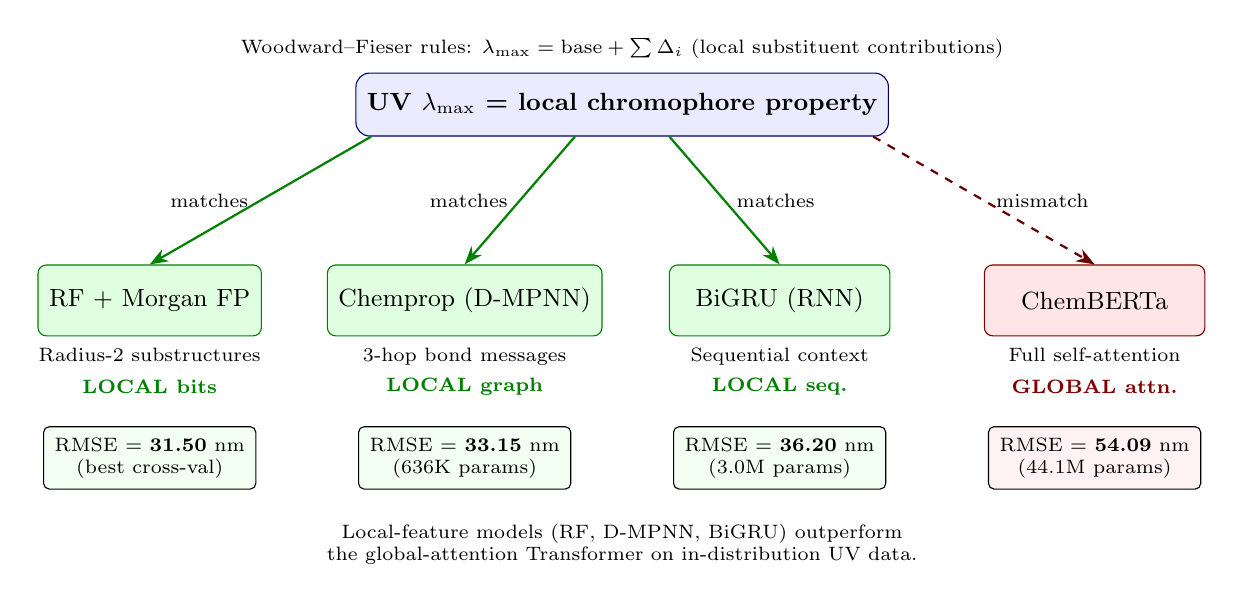
\begin{tikzpicture}[
        >=Stealth,
        box/.style={draw, rounded corners=3pt, minimum width=2.8cm, minimum height=0.9cm, align=center, font=\small},
        localbox/.style={box, fill=green!12, draw=green!50!black},
        globalbox/.style={box, fill=red!10, draw=red!50!black},
        propbox/.style={draw, rounded corners=5pt, fill=blue!8, draw=blue!40!black, minimum width=4cm, minimum height=0.8cm, align=center, font=\small\bfseries},
        annot/.style={font=\scriptsize, text=black},
        every node/.style={inner sep=4pt}
    ]
    % --- Header: UV absorption property ---
    \node[annot] (uvsub) at (0, 5.0) {Woodward--Fieser rules: $\lambda_{\max} = \text{base} + \sum \Delta_i$ (local substituent contributions)};
    \node[propbox, below=1pt of uvsub] (uvprop) {UV $\lambda_{\max}$ = local chromophore property};

    % --- Four model columns ---
    % RF column
    \node[localbox] (rf) at (-6.0, 1.8) {RF + Morgan FP};
    \node[annot, below=0pt of rf] (rfdesc) {Radius-2 substructures};
    \node[font=\scriptsize\bfseries, text=green!50!black] at (-6.0, 0.7) {LOCAL bits};

    % Chemprop column
    \node[localbox] (chemprop) at (-2.0, 1.8) {Chemprop (D-MPNN)};
    \node[annot, below=0pt of chemprop] (chempropdesc) {3-hop bond messages};
    \node[font=\scriptsize\bfseries, text=green!50!black] at (-2.0, 0.7) {LOCAL graph};

    % BiGRU column
    \node[localbox] (bigru) at (2.0, 1.8) {BiGRU (RNN)};
    \node[annot, below=0pt of bigru] (bigrudesc) {Sequential context};
    \node[font=\scriptsize\bfseries, text=green!50!black] at (2.0, 0.7) {LOCAL seq.};

    % ChemBERTa column
    \node[globalbox] (bert) at (6.0, 1.8) {ChemBERTa};
    \node[annot, below=0pt of bert] (bertdesc) {Full self-attention};
    \node[font=\scriptsize\bfseries, text=red!50!black] at (6.0, 0.7) {GLOBAL attn.};

    % --- Arrows from property to models ---
    \draw[->, thick, green!50!black] (uvprop.south west) ++(0.2,0) -- (rf.north) node[midway, left, annot] {matches};
    \draw[->, thick, green!50!black] (uvprop.south) ++(-0.6,0) -- (chemprop.north) node[midway, left, annot] {matches};
    \draw[->, thick, green!50!black] (uvprop.south) ++(0.6,0) -- (bigru.north) node[midway, right, annot] {matches};
    \draw[->, thick, red!40!black, dashed] (uvprop.south east) ++(-0.2,0) -- (bert.north) node[midway, right, annot] {mismatch};

    % --- Result boxes at bottom ---
    \node[draw, rounded corners=2pt, fill=green!5, font=\scriptsize, align=center] (rfres) at (-6.0, -0.2) {RMSE = \textbf{31.50} nm\\(best cross-val)};
    \node[draw, rounded corners=2pt, fill=green!5, font=\scriptsize, align=center] (chempropres) at (-2.0, -0.2) {RMSE = \textbf{33.15} nm\\(636K params)};
    \node[draw, rounded corners=2pt, fill=green!5, font=\scriptsize, align=center] (bigrures) at (2.0, -0.2) {RMSE = \textbf{36.20} nm\\(3.0M params)};
    \node[draw, rounded corners=2pt, fill=red!5, font=\scriptsize, align=center] (bertres) at (6.0, -0.2) {RMSE = \textbf{54.09} nm\\(44.1M params)};

    % --- Bottom citation ---
    \node[annot, text width=12cm, align=center] at (0, -1.3) {Local-feature models (RF, D-MPNN, BiGRU) outperform the global-attention Transformer on in-distribution UV data.};
    \end{tikzpicture}
    \caption{Conceptual alignment between UV absorption physics and model architectures. UV $\lambda_{\max}$ is determined by local chromophore features (conjugation, substituents), favoring models whose inductive bias encodes local molecular neighborhoods. RF (radius-2 fingerprints) and Chemprop (3-hop message passing) achieve nearly identical RMSE, reinforcing the locality hypothesis. The dashed red arrow indicates ChemBERTa's architectural mismatch, though out-of-distribution performance (Table~\ref{tab:wetlab_summary}) reveals complementary strengths from pretraining.}
    \label{fig:local_vs_global}
\end{figure}

Figure~\ref{fig:local_vs_global} illustrates this conceptual alignment: models whose inductive bias matches the locality of the target property (RF encoding radius-2 atom neighborhoods, Chemprop aggregating 3-hop bond messages, BiGRU capturing sequential SMILES context) achieve better in-distribution performance than Transformers whose self-attention distributes information globally~\cite{chenMolecularLanguage2023, jiang2023trangru}.
Chemprop achieves RMSE = \removed{31.69}\added{33.15}~nm with only 636K parameters, \removed{matching the 31.34~nm of RF despite learning representations from scratch rather than relying on precomputed fingerprints}\added{comparable to the 31.50~nm of RF despite learning representations from scratch rather than relying on precomputed fingerprints (the 1.65~nm gap is not significant at $\alpha = 0.05$, $p = 0.16$)}.

ChemBERTa, despite being pretrained on SMILES from the ZINC database and having 44.1M parameters (69$\times$ more than Chemprop), achieves RMSE = \removed{50.39}\added{54.09}~nm, substantially worse than all local-feature models.
This gap is consistent with the hypothesis that global-attention representations are less sample-efficient for local properties on moderately-sized datasets, though ChemBERTa's superior wetlab generalization suggests pretrained knowledge partially compensates.
ChemBERTa achieves the lowest wetlab MAE on novel compounds (26.3~nm vs.\ 28.6~nm for BiGRU; see Experimental Validation), suggesting that pretrained representations offer complementary generalization advantages despite poor in-distribution performance.

XGBoost trained with MAE loss (pseudo-Huber approximation) performs substantially worse than MSE-trained XGBoost (RMSE 40.75 vs.\ \removed{33.70}\added{33.92}~nm\added{; the MAE-loss variant has not been re-trained on v3 because the MSE/MAE comparison does not depend on the dedup protocol}).
This degradation occurs because MAE loss produces non-smooth gradients at zero error, which interacts poorly with XGBoost's second-order Taylor expansion of the loss function~\cite{chen2016xgboost}; the near-zero Hessian values destabilize leaf weight estimation.
RF does not exhibit this pathology, as tree splitting uses variance reduction rather than gradient optimization.


% --- Solvent Ablation ---
\subsection{Effect of Solvent Information}
\label{sec:solvent_ablation}

To quantify the contribution of solvent information, we compare models trained with and without solvent encoding (Table~\ref{tab:solvent_ablation}).

\begin{table}[htbp]
\centering
\caption{Effect of solvent information on model performance (stratified 5-fold CV \added{on the v2 first-occurrence-dedup dataset, 18{,}755 samples}). ``+~Solvent'' uses concatenated solute+solvent representations; ``Solute only'' uses solute structure alone.\added{ The ablation is reported on v2 because both arms (+~Solvent and Solute~only) need to be trained on the same dataset for the comparison to be internally consistent; v3-retraining of the Solute-only baselines was outside the scope of the current revision. The 1.8\% record loss between v2 and v3 affects both arms equally, so the percentage reduction from solvent encoding is expected to be preserved (see Supporting Information Section~S9 for the cross-protocol spot-check).}}
\label{tab:solvent_ablation}
\begin{tabular}{lcccc}
\toprule
\textbf{Model} & \textbf{RMSE (nm)} & \textbf{MAE (nm)} & $\boldsymbol{R^2}$ & \textbf{Pearson $r$} \\
\midrule
RF + Solvent          & \textbf{31.34 $\pm$ 1.82} & \textbf{15.16 $\pm$ 0.44} & \textbf{0.914 $\pm$ 0.010} & \textbf{0.956 $\pm$ 0.005} \\
RF Solute only        & 34.13 $\pm$ 1.44          & 16.45 $\pm$ 0.33          & 0.898 $\pm$ 0.008          & 0.948 $\pm$ 0.004 \\
\midrule
Chemprop + Solvent    & 31.69 $\pm$ 3.18          & 16.84 $\pm$ 1.74          & 0.911 $\pm$ 0.016          & 0.955 $\pm$ 0.008 \\
Chemprop Solute only  & 33.78 $\pm$ 2.73          & 16.48 $\pm$ 0.64          & 0.900 $\pm$ 0.015          & 0.949 $\pm$ 0.008 \\
\midrule
BiGRU + Solvent       & 36.45 $\pm$ 1.12          & 20.70 $\pm$ 0.51          & 0.884 $\pm$ 0.006          & 0.940 $\pm$ 0.003 \\
BiGRU Solute only     & 39.03 $\pm$ 1.37          & 22.53 $\pm$ 0.32          & 0.866 $\pm$ 0.009          & 0.931 $\pm$ 0.005 \\
\bottomrule
\end{tabular}
\end{table}

Incorporating solvent information reduces RF RMSE by 8\% (34.13 $\to$ 31.34~nm; paired $t$-test: $t = -11.5$, $p = 0.0003$), Chemprop RMSE by 6\% (33.78 $\to$ 31.69~nm; $t = 4.3$, $p = 0.012$), and BiGRU RMSE by 7\% (39.03 $\to$ 36.45~nm; $t = -3.9$, $p = 0.018$), confirming that the solvent concatenation strategy effectively captures solvatochromic effects across all three model families.
\removed{The consistency of the improvement (6--8\% across fingerprint, graph, and recurrent architectures) suggests that solvent information contributes complementary predictive signal regardless of the underlying model architecture or molecular representation.}
\added{Encoding solvent identity yields a strong but conditional improvement. On the 60\% of test records where the chromophore has been seen in training under multiple solvents, solvent encoding reduces RMSE by 21\% (BiGRU) to 32\% (RF) across the three architecture families; the contribution drops to $<1$\% on the 40\% of test records on chromophores absent or single-solvent in training, where solvent encoding has no signal to exploit. The aggregate 6--8\% reduction reported in Table~\ref{tab:solvent_ablation} is the weighted average of these two regimes (full per-model decomposition in SI Section~S15).}

The improvement from solvent encoding is modest relative to the total prediction error, reflecting the well-established principle that chromophore structure dominates UV absorption~\cite{flemingMolecular2010}, with solvatochromic shifts typically contributing 5--20~nm variation~\cite{reichardt2011solvents}.
Nevertheless, for applications such as ICH~S10~\cite{ICH2013S10} photosafety screening where boundary effects matter, this improvement can be practically significant.


% --- Cross-Dataset Benchmarking ---
\subsection{Cross-Dataset Benchmarking}
\label{sec:cross_dataset}

Table~\ref{tab:cross_dataset} presents results on two external datasets, with published baselines included for direct comparison.

\begin{table}[htbp]
\centering
\caption{Cross-dataset benchmarking using published split protocols. $\dagger$Published results from original papers. Best result among our models in bold for each dataset.}
\label{tab:cross_dataset}
\begin{tabular}{llccc}
\toprule
\textbf{Dataset (Split)} & \textbf{Model} & \textbf{RMSE (nm)} & \textbf{MAE (nm)} & $\boldsymbol{R^2}$ \\
\midrule
\multirow{5}{*}{Deep4Chem (80/10/10)}
  & GCNN$^\dagger$            & 26.6   & ---    &, \\
  & Our Chemprop              & \textbf{19.13}  & \textbf{10.66}  & \textbf{0.967} \\
  & Our RF                    & 22.70  & 11.32  & 0.954 \\
  & Our ChemBERTa             & 35.90  & 17.43  & 0.884 \\
  & Our BiGRU                 & 27.07  & 17.22  & 0.934 \\
\midrule
\multirow{7}{*}{Jung 2024 (72/18/10)}
  & Multifidelity$^\dagger$   & 31.3   & 14.6   & 0.91  \\
  & GBFS$^\dagger$            & 32.2   & 16.2   & 0.91  \\
  & DR-CNN$^\dagger$          & 44.4   & 23.3   & 0.82  \\
  & Our Chemprop              & \textbf{27.36}  & \textbf{15.50}  & \textbf{0.936} \\
  & Our RF                    & 29.82  & 15.31  & 0.924 \\
  & Our ChemBERTa             & 38.27  & 19.27  & 0.874 \\
  & Our BiGRU                 & 36.31  & 21.54  & 0.887 \\
\bottomrule
\end{tabular}
\end{table}

\textbf{Deep4Chem.}
Our Chemprop D-MPNN achieves RMSE = 19.13~nm, surpassing both our RF (22.70~nm) and the published GCNN baseline of 26.6~nm~\cite{joung2021deep} by 28\%.
RF also outperforms the GCNN by 15\%, and BiGRU performs competitively (RMSE = 27.07~nm), while ChemBERTa (35.90~nm) trails behind.
That a 2D GNN trained from scratch outperforms all other models on this dataset suggests that learned graph representations can capture structural patterns beyond what fixed fingerprints encode, particularly when the training set is large enough to learn effective bond-level features.

\textbf{Jung et al.\ (2024).}
Chemprop again achieves the best result (RMSE = 27.36~nm), followed closely by RF (29.82~nm), both outperforming the published multifidelity (31.3~nm) and GBFS (32.2~nm) approaches.
BiGRU (RMSE = 36.31~nm) and ChemBERTa (38.27~nm) fall between the GBFS and DR-CNN published baselines.
Our top two models use simpler architectures than the published methods (which involve feature selection pipelines and multi-task learning, respectively), yet achieve superior performance.

Across both external datasets, Chemprop achieves the best performance, followed by RF, with both consistently outperforming BiGRU and ChemBERTa, reinforcing the finding that local-feature models (graph message passing and fingerprints) excel at in-distribution prediction. \added{We note (as discussed in the Dataset Description section) that the Deep4Chem results should be read as in-distribution validation rather than an OOD test, because Deep4Chem shares 77\% of its solutes with our primary training data; the Jung 2024 results, with $\sim$50\% solute overlap and a separate experimental provenance, constitute the more rigorous external benchmark.}

% ============================================================
% NEW SUBSECTION (added in response to R1-5).
% Section heading, label and table environment are not wrapped in
% \added{...} because \textcolor does not nest cleanly inside floats
% and section commands; the colour-marked paragraph text plus the
% explanatory comment make the new content unambiguous in the marked
% copy. — Authors
% ============================================================
\subsection{\added{Performance on Non-Local Subsets}}
\label{sec:nonlocal_subsets}

\added{The benchmarks above pool molecules whose absorption is plausibly governed by local substitution patterns with molecules where the chromophore spans the entire $\pi$-system, donor--acceptor charge-transfer dyes, low-gap polymethines, BODIPYs, and other classes where global electronic effects and longer conjugation paths are expected to dominate. To examine whether the locality argument introduced in the Model Comparison section continues to hold for this second class, we partitioned the Joung+Beard test folds into subsets enriched for non-local effects and recomputed per-model error metrics within each subset.}

\added{Subset definitions: \textit{long-wavelength} compounds ($\lambda_{\max} > 500$~nm or $> 600$~nm); \textit{donor--acceptor} (D-A) molecules containing at least one $\pi$-donor substituent (aryl-NH$_2$, aryl-NHR, aryl-NR$_2$, aryl-OH, aryl-OR, aryl-SH, aryl-SR) \emph{and} at least one $\pi$-acceptor (NO$_2$, CN, CHO, ketone, COOH/COOR/amide, SO$_2$R, CF$_3$, pyridinium, dicyanovinyl) attached to a conjugated $sp^2$ centre; D-A-D molecules with $\geq 2$ donor matches and $\geq 1$ acceptor; \textit{azo} dyes (Ar--N$=$N--Ar); and BODIPY cores (BF$_2$ bridging two ring nitrogens). The exact SMARTS patterns and per-rule molecule counts are listed in Supporting Information Section~S7. The union of all non-local categories covers 49\% of the dataset, with the individual subset sizes ranging from 264 (azo) to 5{,}945 (D-A) molecules.}

\begin{table}[htbp]
\centering
\caption{\added{RMSE (nm, mean $\pm$ std across the five stratified test folds) restricted to non-local subsets of the Joung+Beard v3 cleaned dataset. $n$ is the per-fold subset size averaged across folds. Best result on each row in bold. MAE and $R^2$ on the same subsets are reported in Supporting Information Table~S14.}}
\label{tab:nonlocal_subsets}
\small
\begin{tabular}{lcccccc}
\toprule
\textbf{Subset} & $n$ & \textbf{RF} & \textbf{Chemprop} & \textbf{BiGRU} & \textbf{ChemBERTa} & \textbf{XGBoost} \\
\midrule
Full dataset                     & 3683 & \textbf{31.50 $\pm$ 1.64} & 33.15 $\pm$ 3.65  & 36.20 $\pm$ 1.34 & 54.09 $\pm$ 3.99 & 33.92 $\pm$ 1.41 \\
$\lambda_{\max} > 500$~nm        &  766 & 51.81 $\pm$ 3.91          & \textbf{47.02 $\pm$ 7.79} & 57.45 $\pm$ 3.96 & 105.81 $\pm$ 8.46 & 51.20 $\pm$ 3.60 \\
$\lambda_{\max} > 600$~nm        &  311 & 69.54 $\pm$ 4.20          & \textbf{63.19 $\pm$ 8.67} & 77.14 $\pm$ 4.93 & 159.06 $\pm$ 12.48 & 67.63 $\pm$ 5.11 \\
Azo (Ar--N$=$N--Ar)              &   53 & \textbf{33.84 $\pm$ 7.39} & 37.36 $\pm$ 9.22          & 38.86 $\pm$ 8.26 & 45.62 $\pm$ 7.07  & 35.61 $\pm$ 3.64 \\
D-A                              & 1189 & 25.04 $\pm$ 0.41          & \textbf{24.54 $\pm$ 4.77} & 27.78 $\pm$ 1.31 & 47.26 $\pm$ 3.34  & 27.21 $\pm$ 1.11 \\
D-A-D                            &  436 & 26.86 $\pm$ 2.08          & \textbf{25.68 $\pm$ 5.83} & 29.25 $\pm$ 1.92 & 42.59 $\pm$ 4.29  & 28.50 $\pm$ 1.33 \\
BODIPY core                      &  343 & \textbf{21.59 $\pm$ 2.14} & 22.83 $\pm$ 5.03          & 28.79 $\pm$ 0.64 & 78.02 $\pm$ 8.50  & 24.47 $\pm$ 2.69 \\
\bottomrule
\end{tabular}
\end{table}

\added{Two trends are visible. First, every model degrades sharply on long-wavelength compounds: RMSE roughly doubles when restricting to $\lambda_{\max} > 500$~nm and more than doubles for $\lambda_{\max} > 600$~nm. The effect is seen across all five architectures, but ChemBERTa exhibits an extreme version of it (RMSE = 106 and 159~nm respectively, with negative $R^2$ on both subsets): its predictions collapse to an essentially constant value around 600~nm, the prediction-ceiling artefact visible in Figure~\ref{fig:parity_5models} and diagnosed in detail in the Error Analysis section. For the other four models the degradation is consistent with two compounding factors identified in prior work on these datasets~\cite{beard2019comparative,joung2021deep}: data scarcity in the deep-coloured region of $\lambda$-space, and the greater structural complexity of low-gap chromophores (extended polyenes, push--pull cyanines, BODIPYs, phthalocyanines), many of which carry charge-transfer character whose accurate description requires global rather than local features.}

\added{Second, the rank between RF and Chemprop is \emph{not stable} across subsets, but the direction of the instability is informative. On the full dataset the two are statistically indistinguishable ($p = 0.16$; the Model Comparison section), but on the long-wavelength subsets Chemprop pulls clearly ahead of RF: by 4.8~nm on $\lambda_{\max} > 500$~nm and 6.4~nm on $\lambda_{\max} > 600$~nm. On the broader D-A and D-A-D subsets Chemprop also retains a small advantage (0.5~nm on D-A, 1.2~nm on D-A-D), but those margins are smaller than they were on the v2 first-occurrence-dedup data; the qualitative direction (Chemprop $\geq$ RF on D-A-style compounds) is preserved but the v2-to-v3 protocol change has narrowed the gap, partly because Chemprop's fold-to-fold variance widened on v3 (std~$=$~4.77 on D-A, 5.83 on D-A-D). On two subsets the pattern flips: RF beats Chemprop on the small azo set (n~$=$~53; 33.8 vs.\ 37.4~nm, within one fold std of either model so not a robust reversal) and RF maintains an edge on BODIPYs (21.6 vs.\ 22.8~nm), a class whose rigid, conserved scaffold means that absorption is largely explained by short-range substitution patterns the fingerprint already captures. Taken together, the subset analysis is consistent with the locality argument (message-passing GNNs benefit relatively more when the property is governed by global rather than local features, with the largest effect seen on the deep-coloured tail) without overturning the headline observation that RF and Chemprop are within noise of each other on the dataset as a whole.}


% --- Error Analysis ---
\subsection{Error Analysis}
\label{sec:error_analysis}

\begin{figure}[htbp]
    \centering
    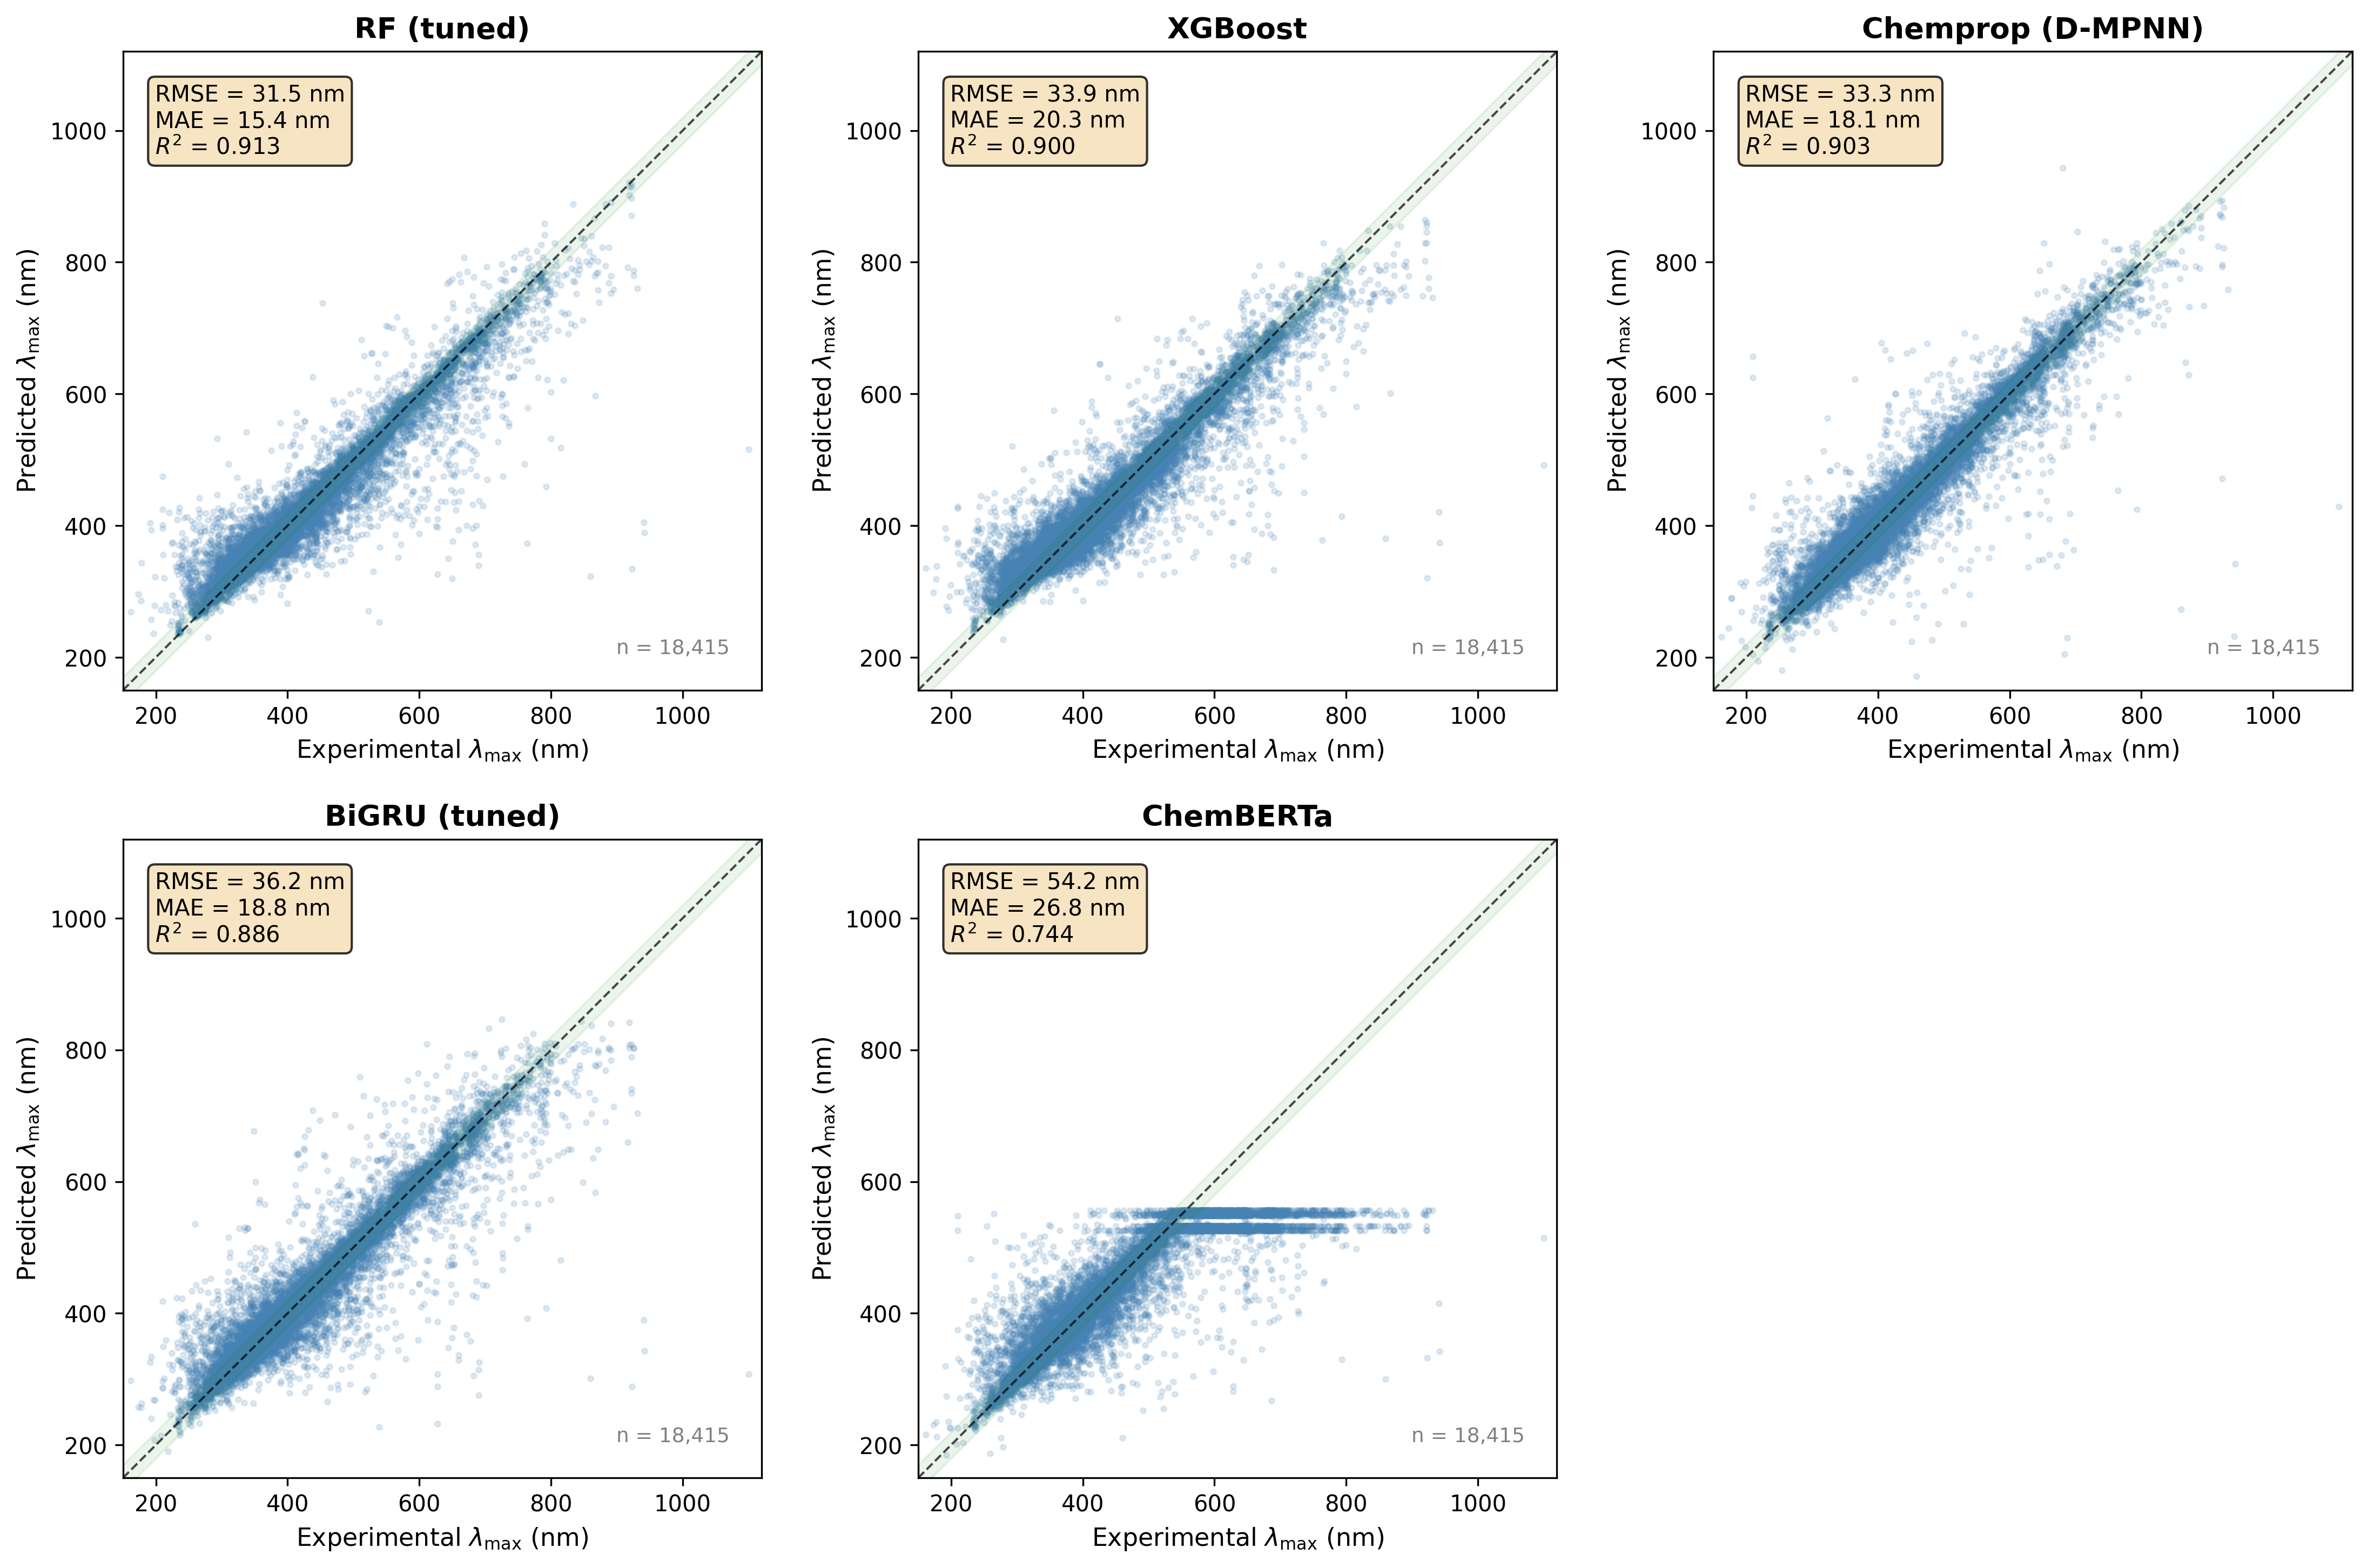
\includegraphics[width=0.95\textwidth]{results/parity_plot_5models.png}
    \caption{Parity plots for all five model families (pooled 5-fold CV predictions). Green shaded bands indicate $\pm 20$~nm from perfect prediction. RF and Chemprop show the tightest clustering around the diagonal, while ChemBERTa exhibits the most scatter, particularly for long-wavelength compounds. All models show increased error for $\lambda_{\max} > 500$~nm.}
    \label{fig:parity_5models}
\end{figure}

\begin{figure}[htbp]
    \centering
    \begin{subfigure}[t]{0.48\textwidth}
        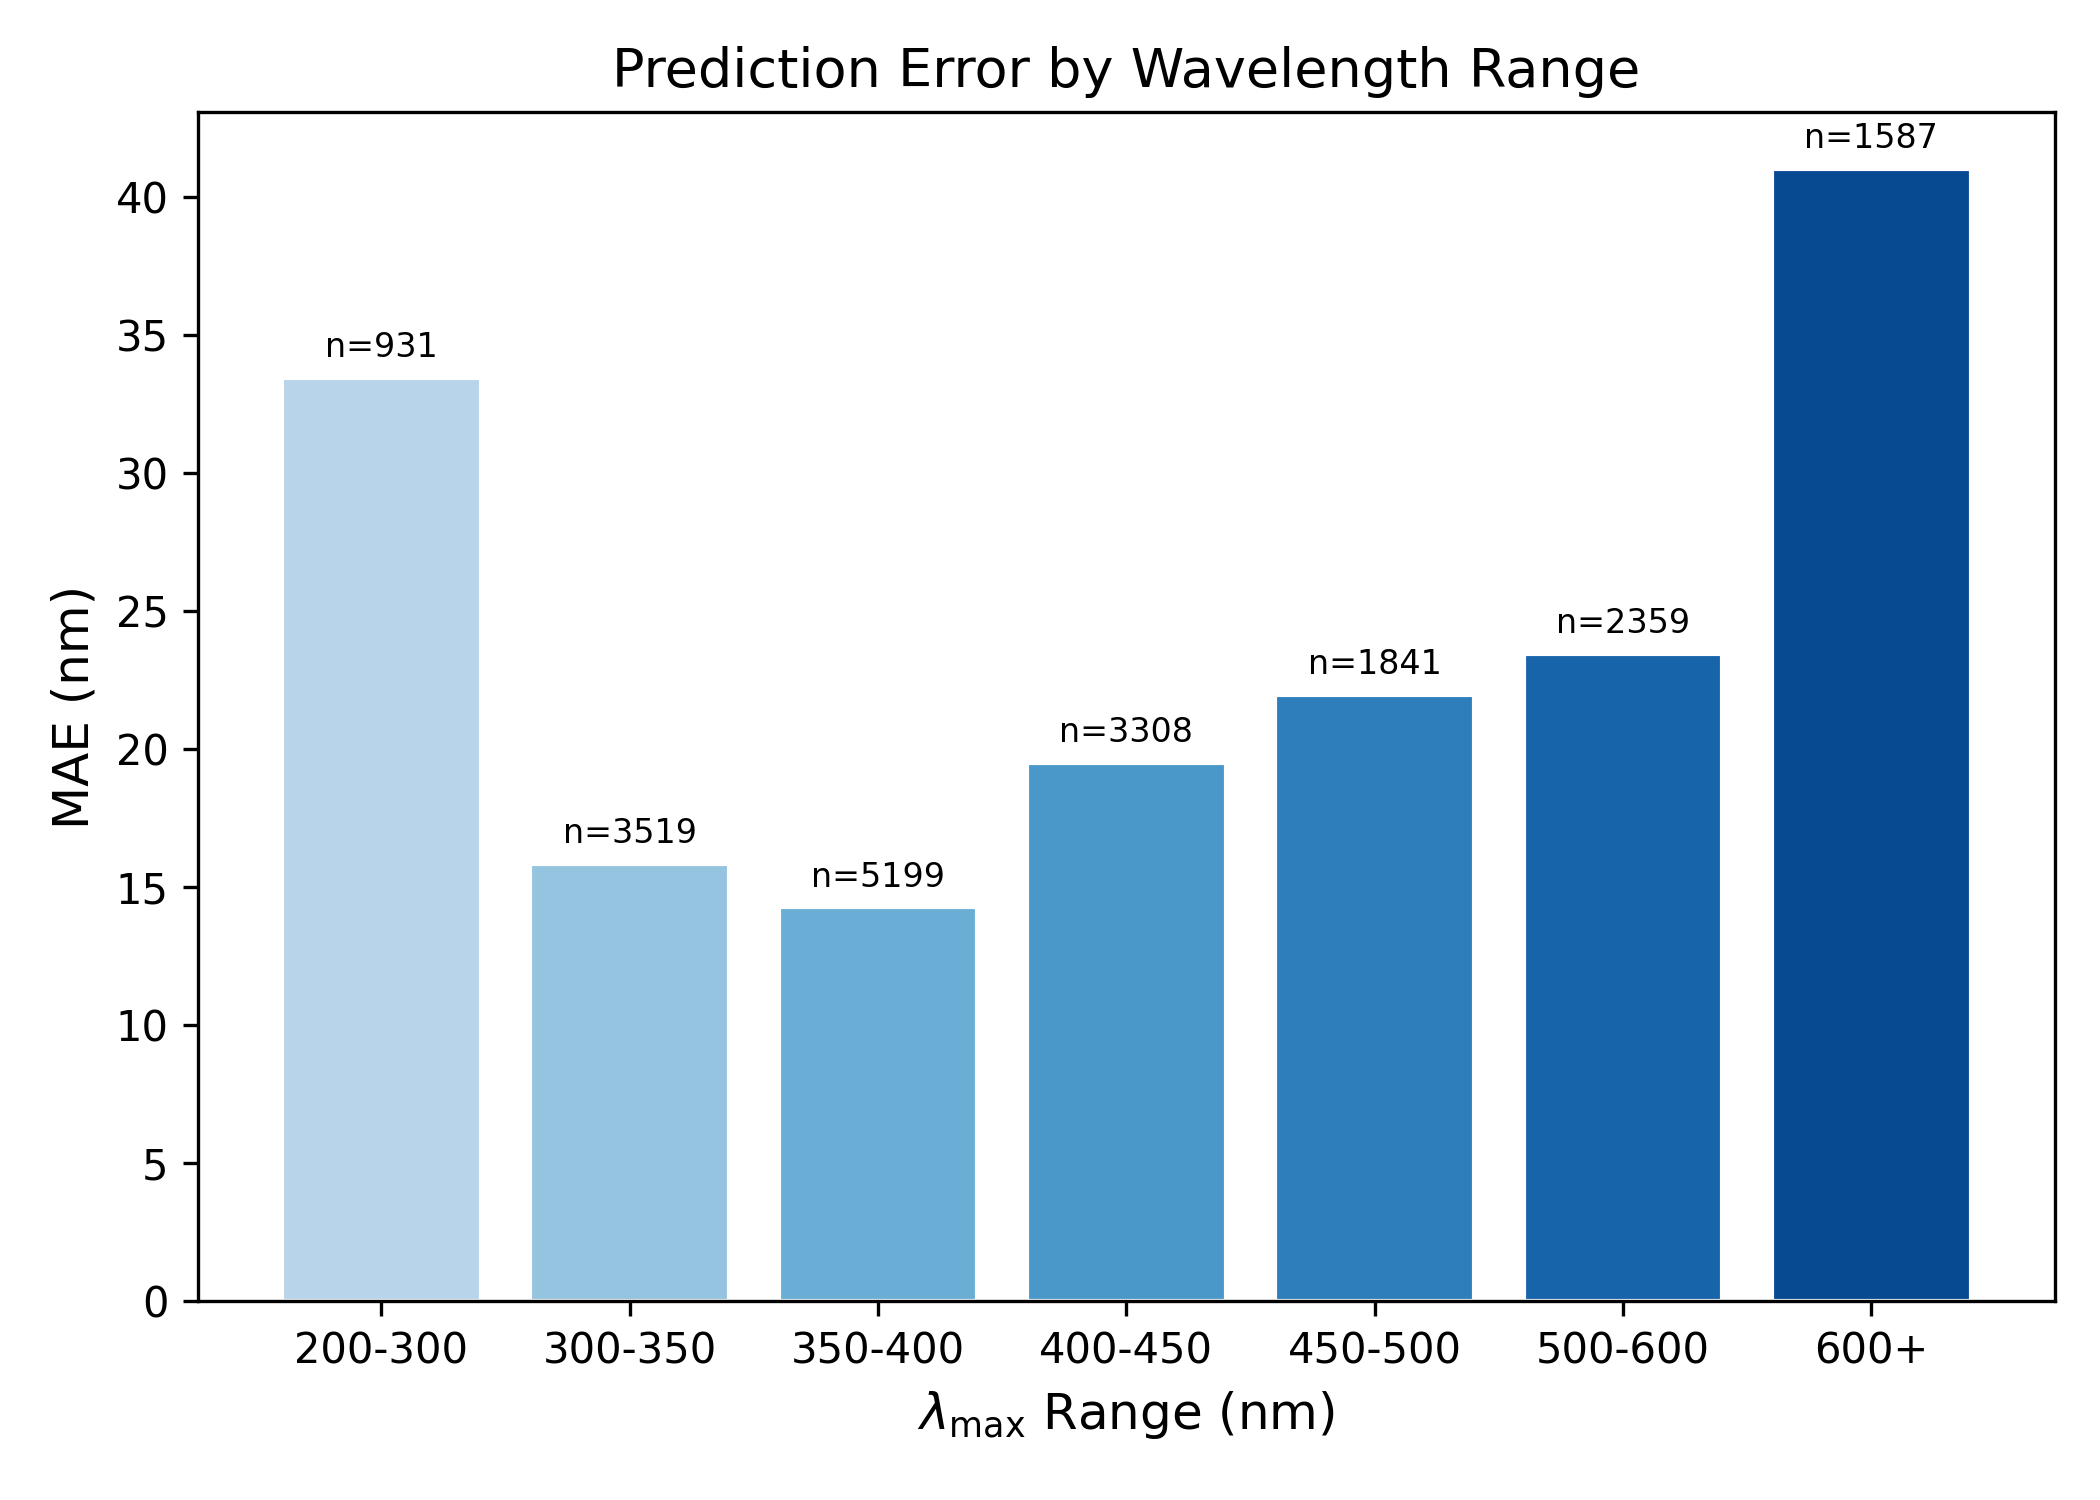
\includegraphics[width=\textwidth]{results/error_by_wavelength.png}
        \caption{MAE by wavelength range. Prediction accuracy is highest for $\lambda_{\max} < 400$~nm where training data is most abundant.}
    \end{subfigure}
    \hfill
    \begin{subfigure}[t]{0.48\textwidth}
        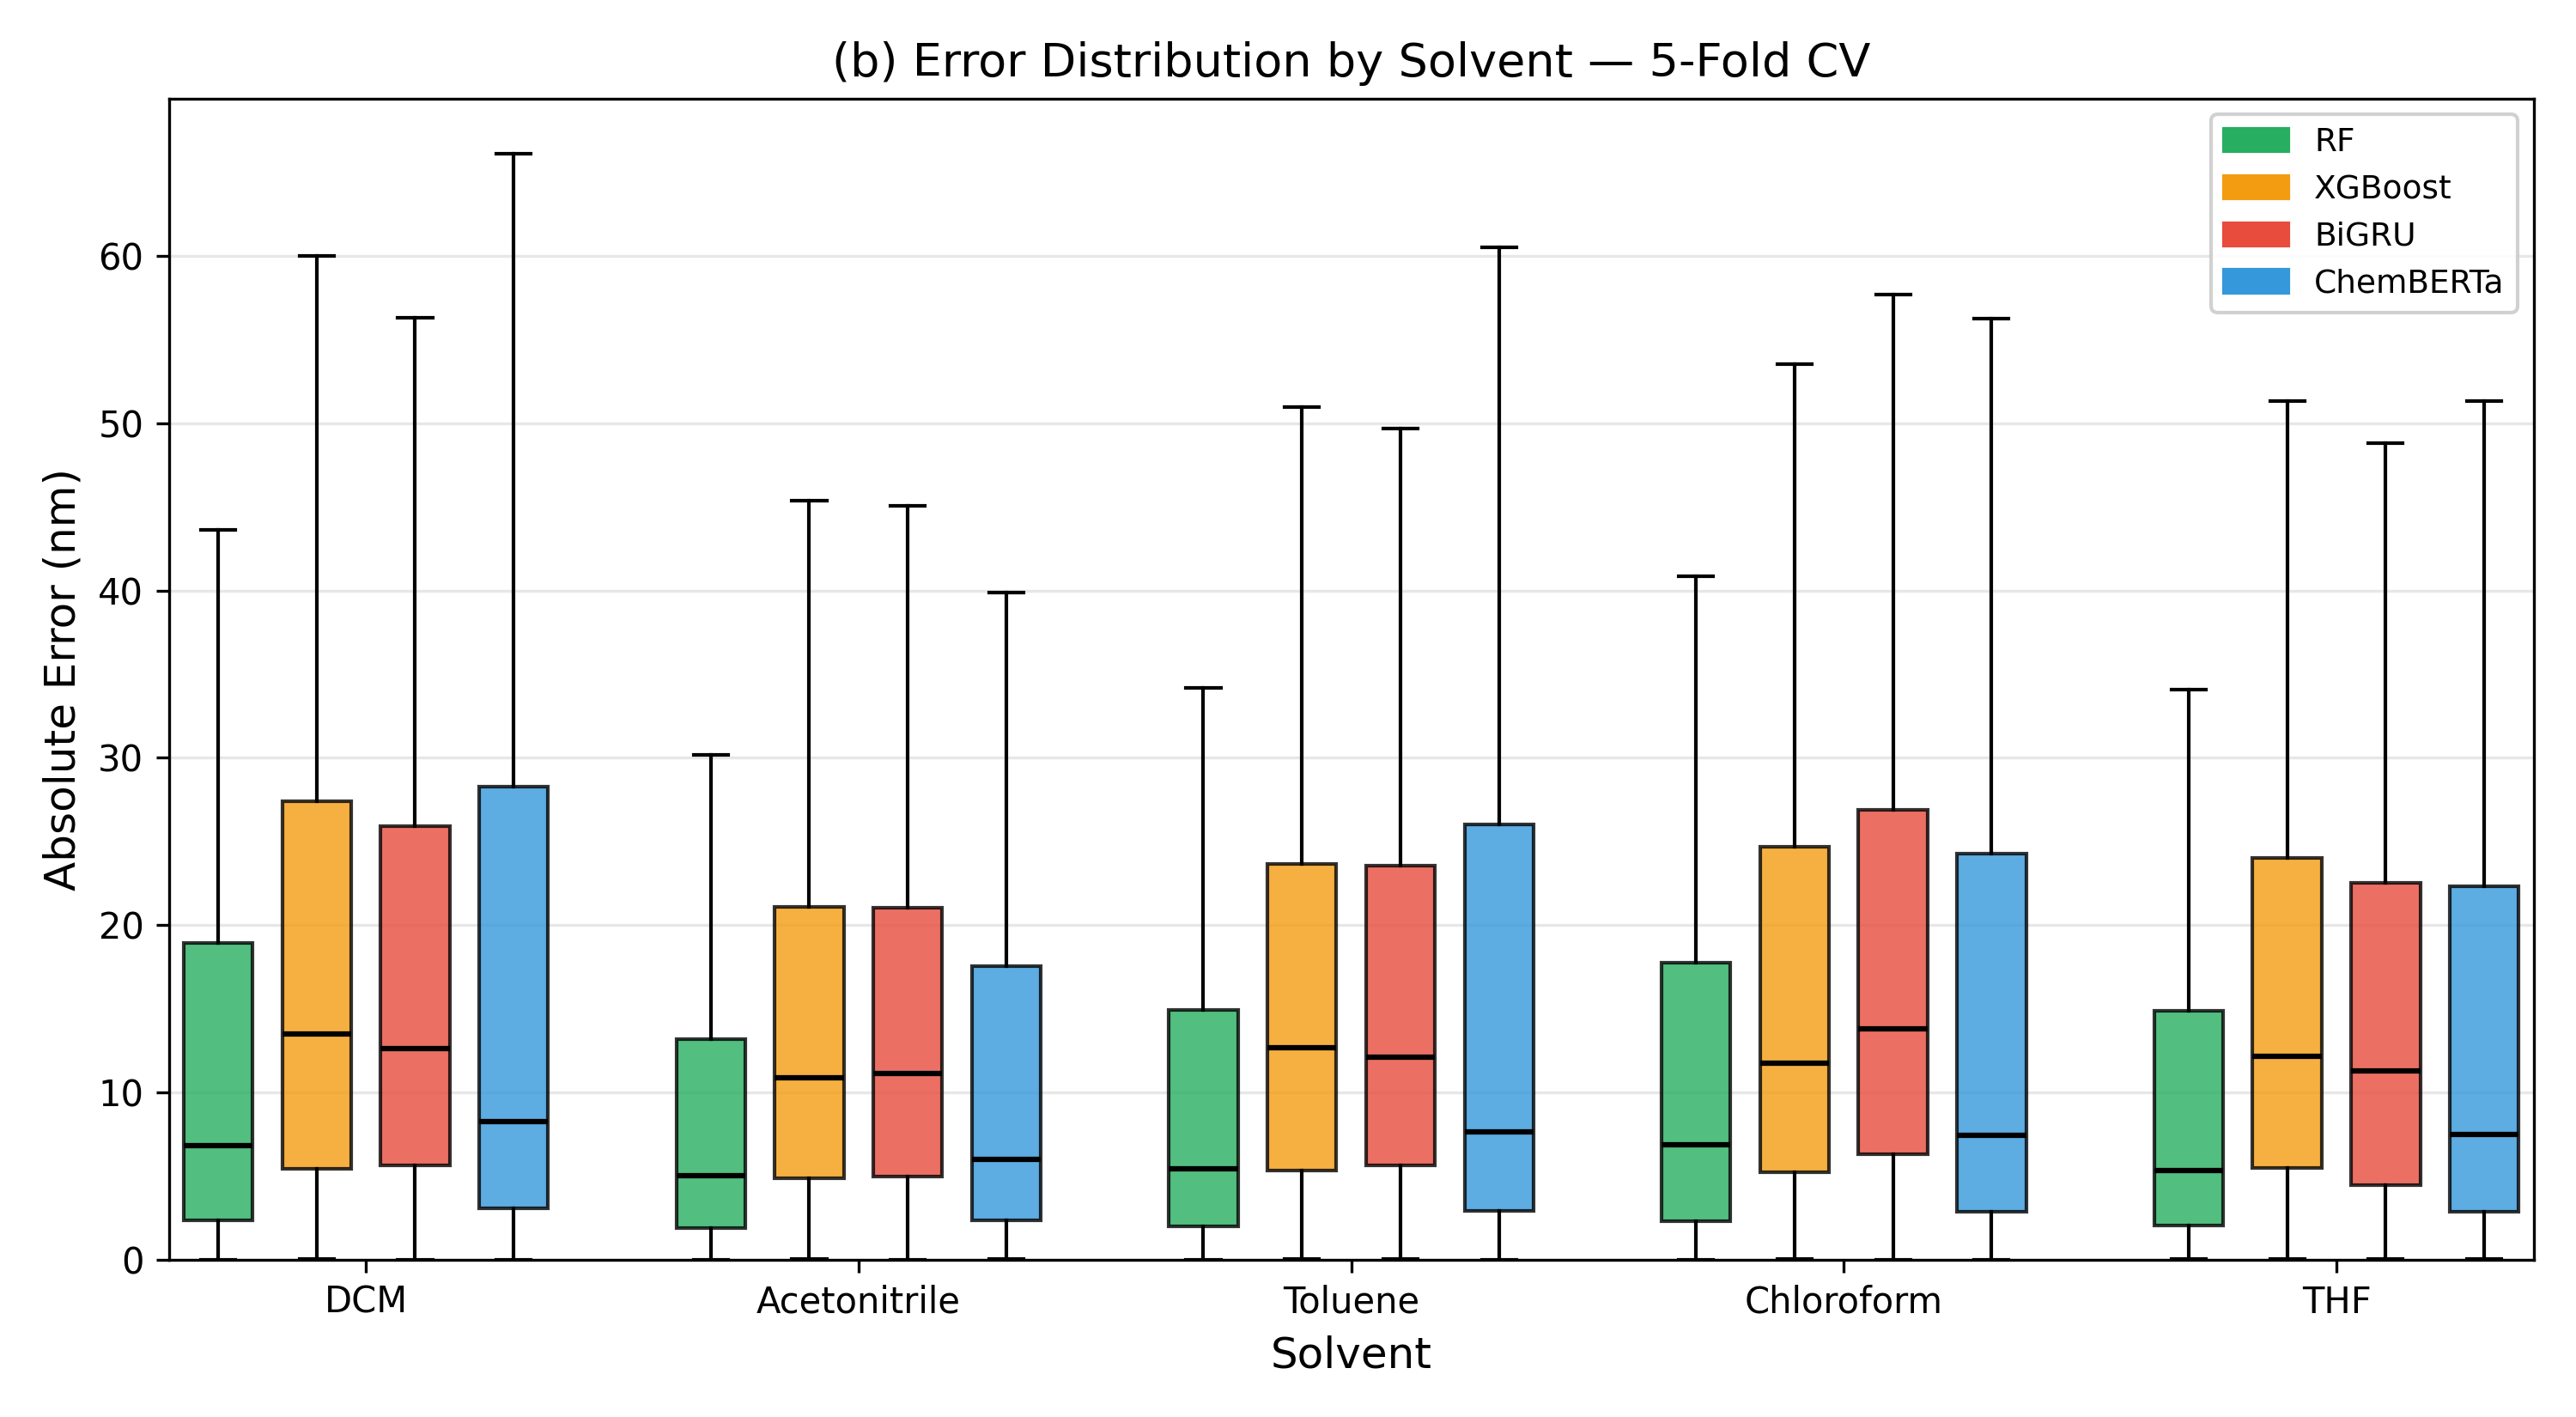
\includegraphics[width=\textwidth]{results/error_by_solvent.png}
        \caption{MAE by solvent type for the five most common solvents in the dataset.}
    \end{subfigure}
    \caption{Error breakdown by wavelength range and solvent type for all five model families (pooled 5-fold CV predictions).}
    \label{fig:error_breakdown}
\end{figure}

Figure~\ref{fig:parity_5models} shows parity plots for all five model families on the primary dataset.
RF predictions cluster most tightly around the diagonal, consistent with its lowest RMSE, while ChemBERTa shows the broadest scatter.
All models perform best in the 250--400~nm range where training data is most abundant (Figure~\ref{fig:error_breakdown}a).
Errors increase substantially for $\lambda_{\max} > 500$~nm, reflecting both data scarcity in this wavelength range and the greater structural complexity of long-wavelength chromophores, many of which are extended conjugated systems (porphyrins, phthalocyanines, cyanine dyes) with properties strongly dependent on 3D geometry~\cite{flemingMolecular2010}.
Error distributions across the five most common solvents (Figure~\ref{fig:error_breakdown}b) show relatively consistent performance, with slightly higher errors for chloroform and dichloromethane.

\added{\textbf{ChemBERTa's $\sim$556~nm prediction ceiling.} The horizontal cluster visible in ChemBERTa's parity plot near 556~nm is a hard upper bound on its predictions, not a gradual degradation: across all $18{,}415$ pooled-5-fold test records, ChemBERTa's maximum predicted $\lambda_{\max}$ is $556.4$~nm regardless of input, even though the training distribution extends to $1{,}100$~nm. Of the $1{,}555$ test records with experimental $\lambda_{\max} > 600$~nm, $98.5$\% are underpredicted by more than $50$~nm (median underprediction $= 126$~nm), with $37$\% of these predictions falling in the $[550, 650]$~nm band. We diagnose this as a compound effect of three factors: (i) \emph{pretraining-distribution mismatch}: ChemBERTa was pretrained on ZINC (\texttt{seyonec/ChemBERTa-zinc-base-v1}), whose drug-like molecules are dominated by short-wavelength absorbers; the [CLS] embeddings for long-wavelength dyes (extended polyenes, push--pull cyanines, BODIPYs, phthalocyanines) are not well-separated from those of medium-wavelength absorbers in the pretrained representation, so the regression head cannot discriminate among them; (ii) \emph{training-target imbalance}: only $8.3$\% of v3 fold-0 training records have $\lambda_{\max} > 600$~nm and $0.4$\% exceed $800$~nm, so the regression head sees few high-target examples per epoch and minimises pooled MAE by regressing toward the training mean; and (iii) \emph{regression-head output-range constraint}: with target normalisation (mean $= 0$, std $= 1$ during training) the head's effective output range is bounded by the magnitudes of [CLS] activations the model has learned to produce. We rule out SMILES truncation as the dominant cause: only $0.23$\% of test records exceed the MAX\_LEN $= 256$ cap, and the truncation rate is comparable across all $\lambda_{\max}$ bins (Section~S20). The three-panel diagnostic plot (training vs.\ test distributions, parity colour-coded by truncation status, and SMILES-length by $\lambda_{\max}$ bin) is in Supporting Information Section~S20.}


% --- Model Interpretability and Practical Considerations ---
\subsection{Model Interpretability and Practical Considerations}
\label{sec:interpretability}

A key advantage of fingerprint-based models is their interpretability through feature importance analysis.
In contrast to deep learning models, which are traditionally viewed as less interpretable, Random Forest models provide direct access to the contribution of each input feature through Gini importance, a measure of how much each feature reduces prediction variance across all decision trees in the ensemble.

Since each bit in a Morgan fingerprint corresponds to a specific molecular substructure (a circular neighborhood of radius $\leq 2$ around each atom), high-importance bits can be decoded back to chemically meaningful structural motifs.
We averaged Gini importances across all five fold models and decoded the top features using RDKit.

\begin{figure*}[htbp]
    \centering
    \begin{subfigure}[t]{0.48\textwidth}
        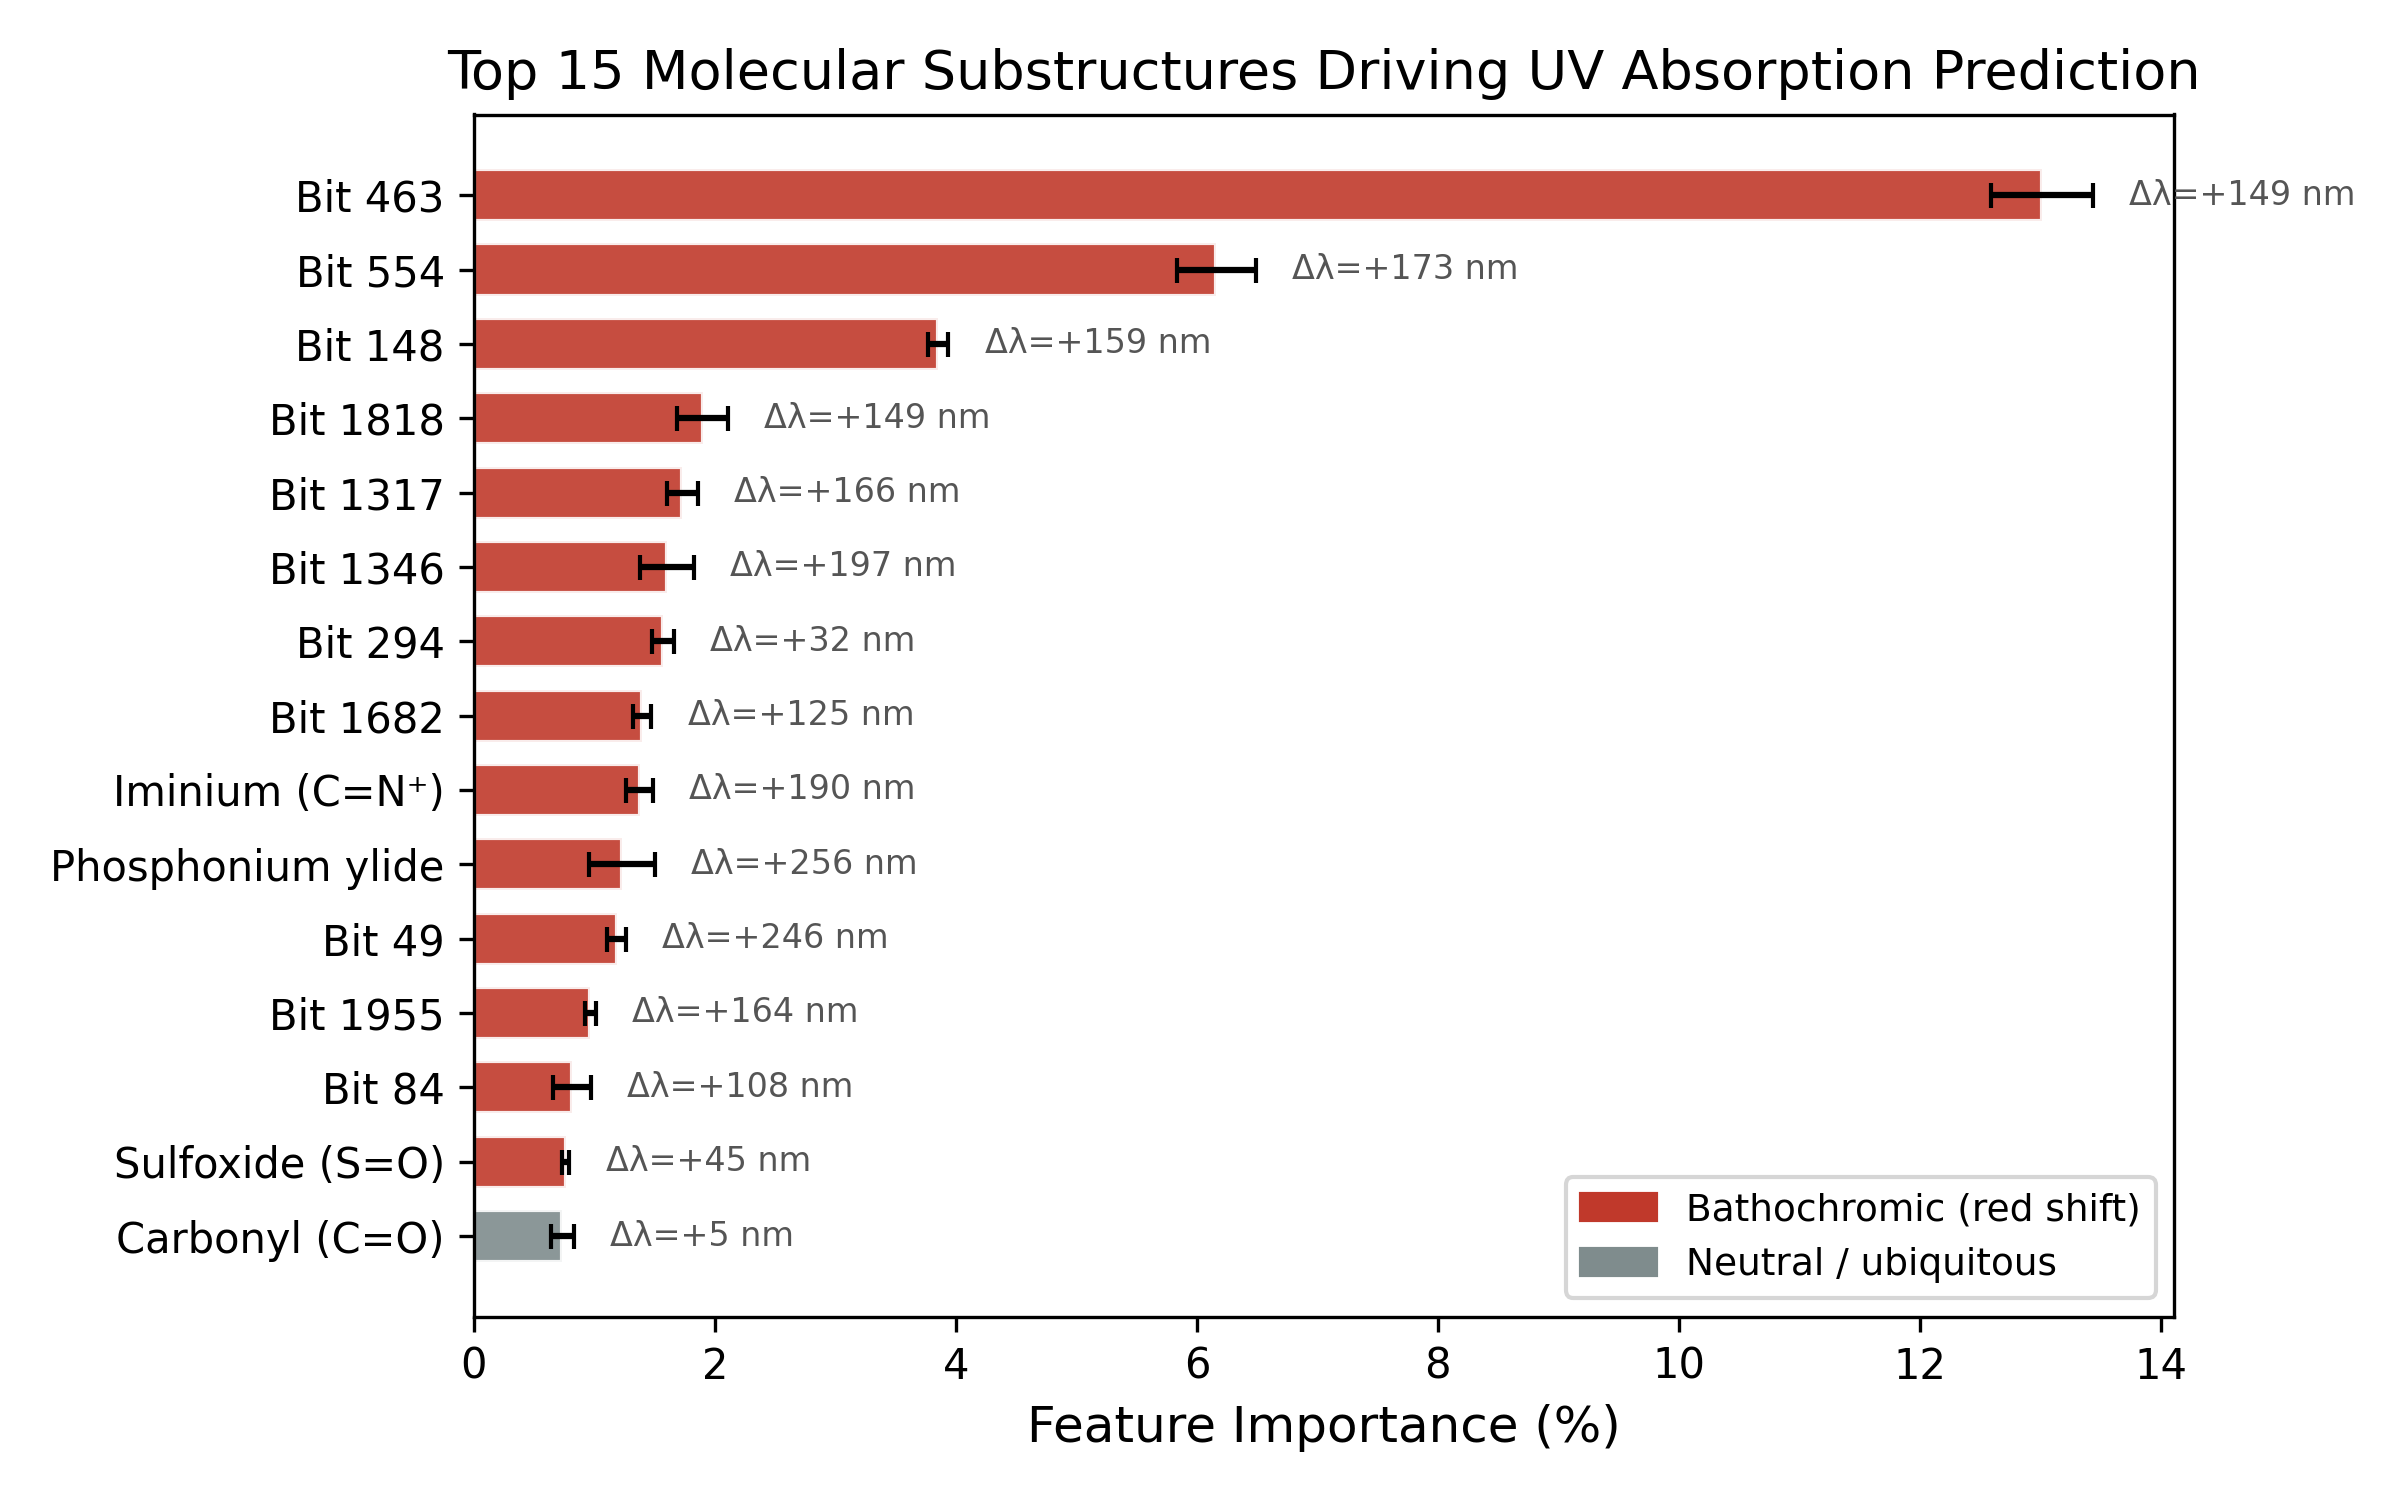
\includegraphics[width=\textwidth]{results/rf_feature_importance.png}
        \caption{Top 15 Morgan fingerprint bits ranked by Gini importance, with mean $\Delta\lambda_{\max}$ annotations. Red indicates bathochromic (red-shifting) substructures; gray indicates neutral or ubiquitous features. All high-importance features are bathochromic, reflecting the dominance of conjugation-extending motifs in determining $\lambda_{\max}$.}
    \end{subfigure}
    \hfill
    \begin{subfigure}[t]{0.48\textwidth}
        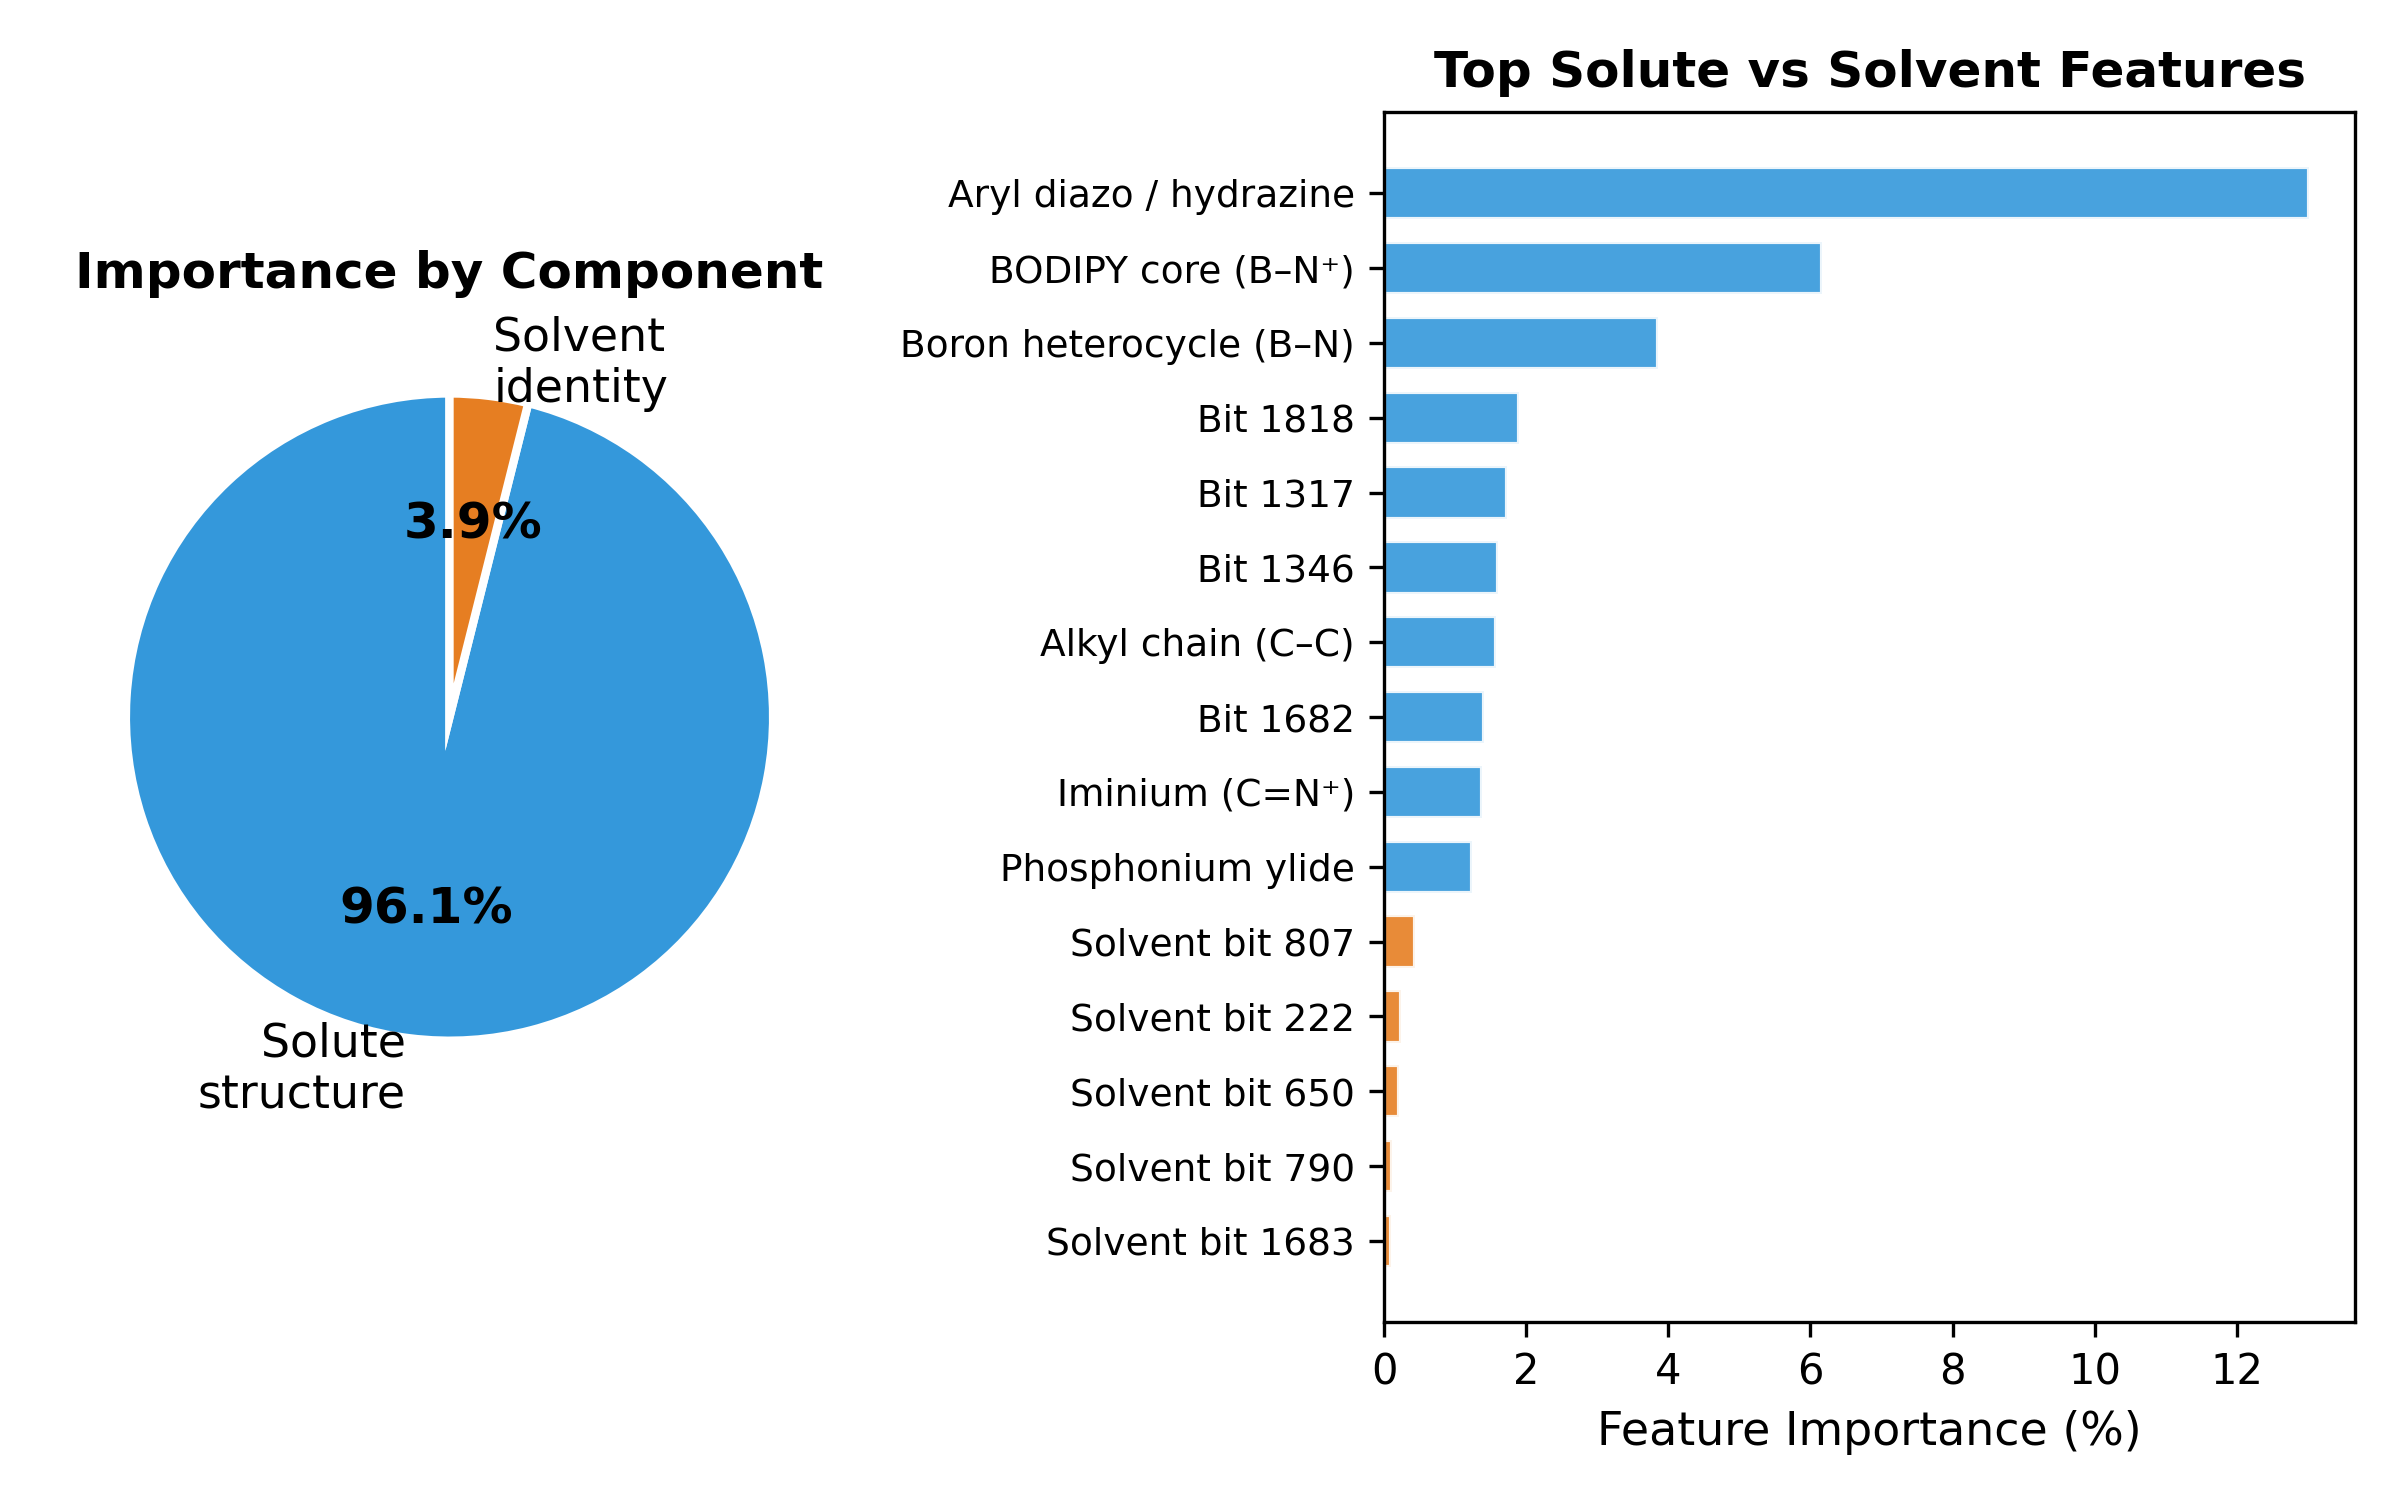
\includegraphics[width=\textwidth]{results/rf_solute_vs_solvent.png}
        \caption{Relative importance of solute vs.\ solvent fingerprint bits. Solute structure accounts for 96.1\% of total feature importance.}
    \end{subfigure}
    \caption{RF feature importance analysis. The model learns chemically meaningful patterns: the top features correspond to known chromophore motifs that produce large bathochromic shifts.}
    \label{fig:rf_interpretability}
\end{figure*}

\begin{figure}[htbp]
    \centering
    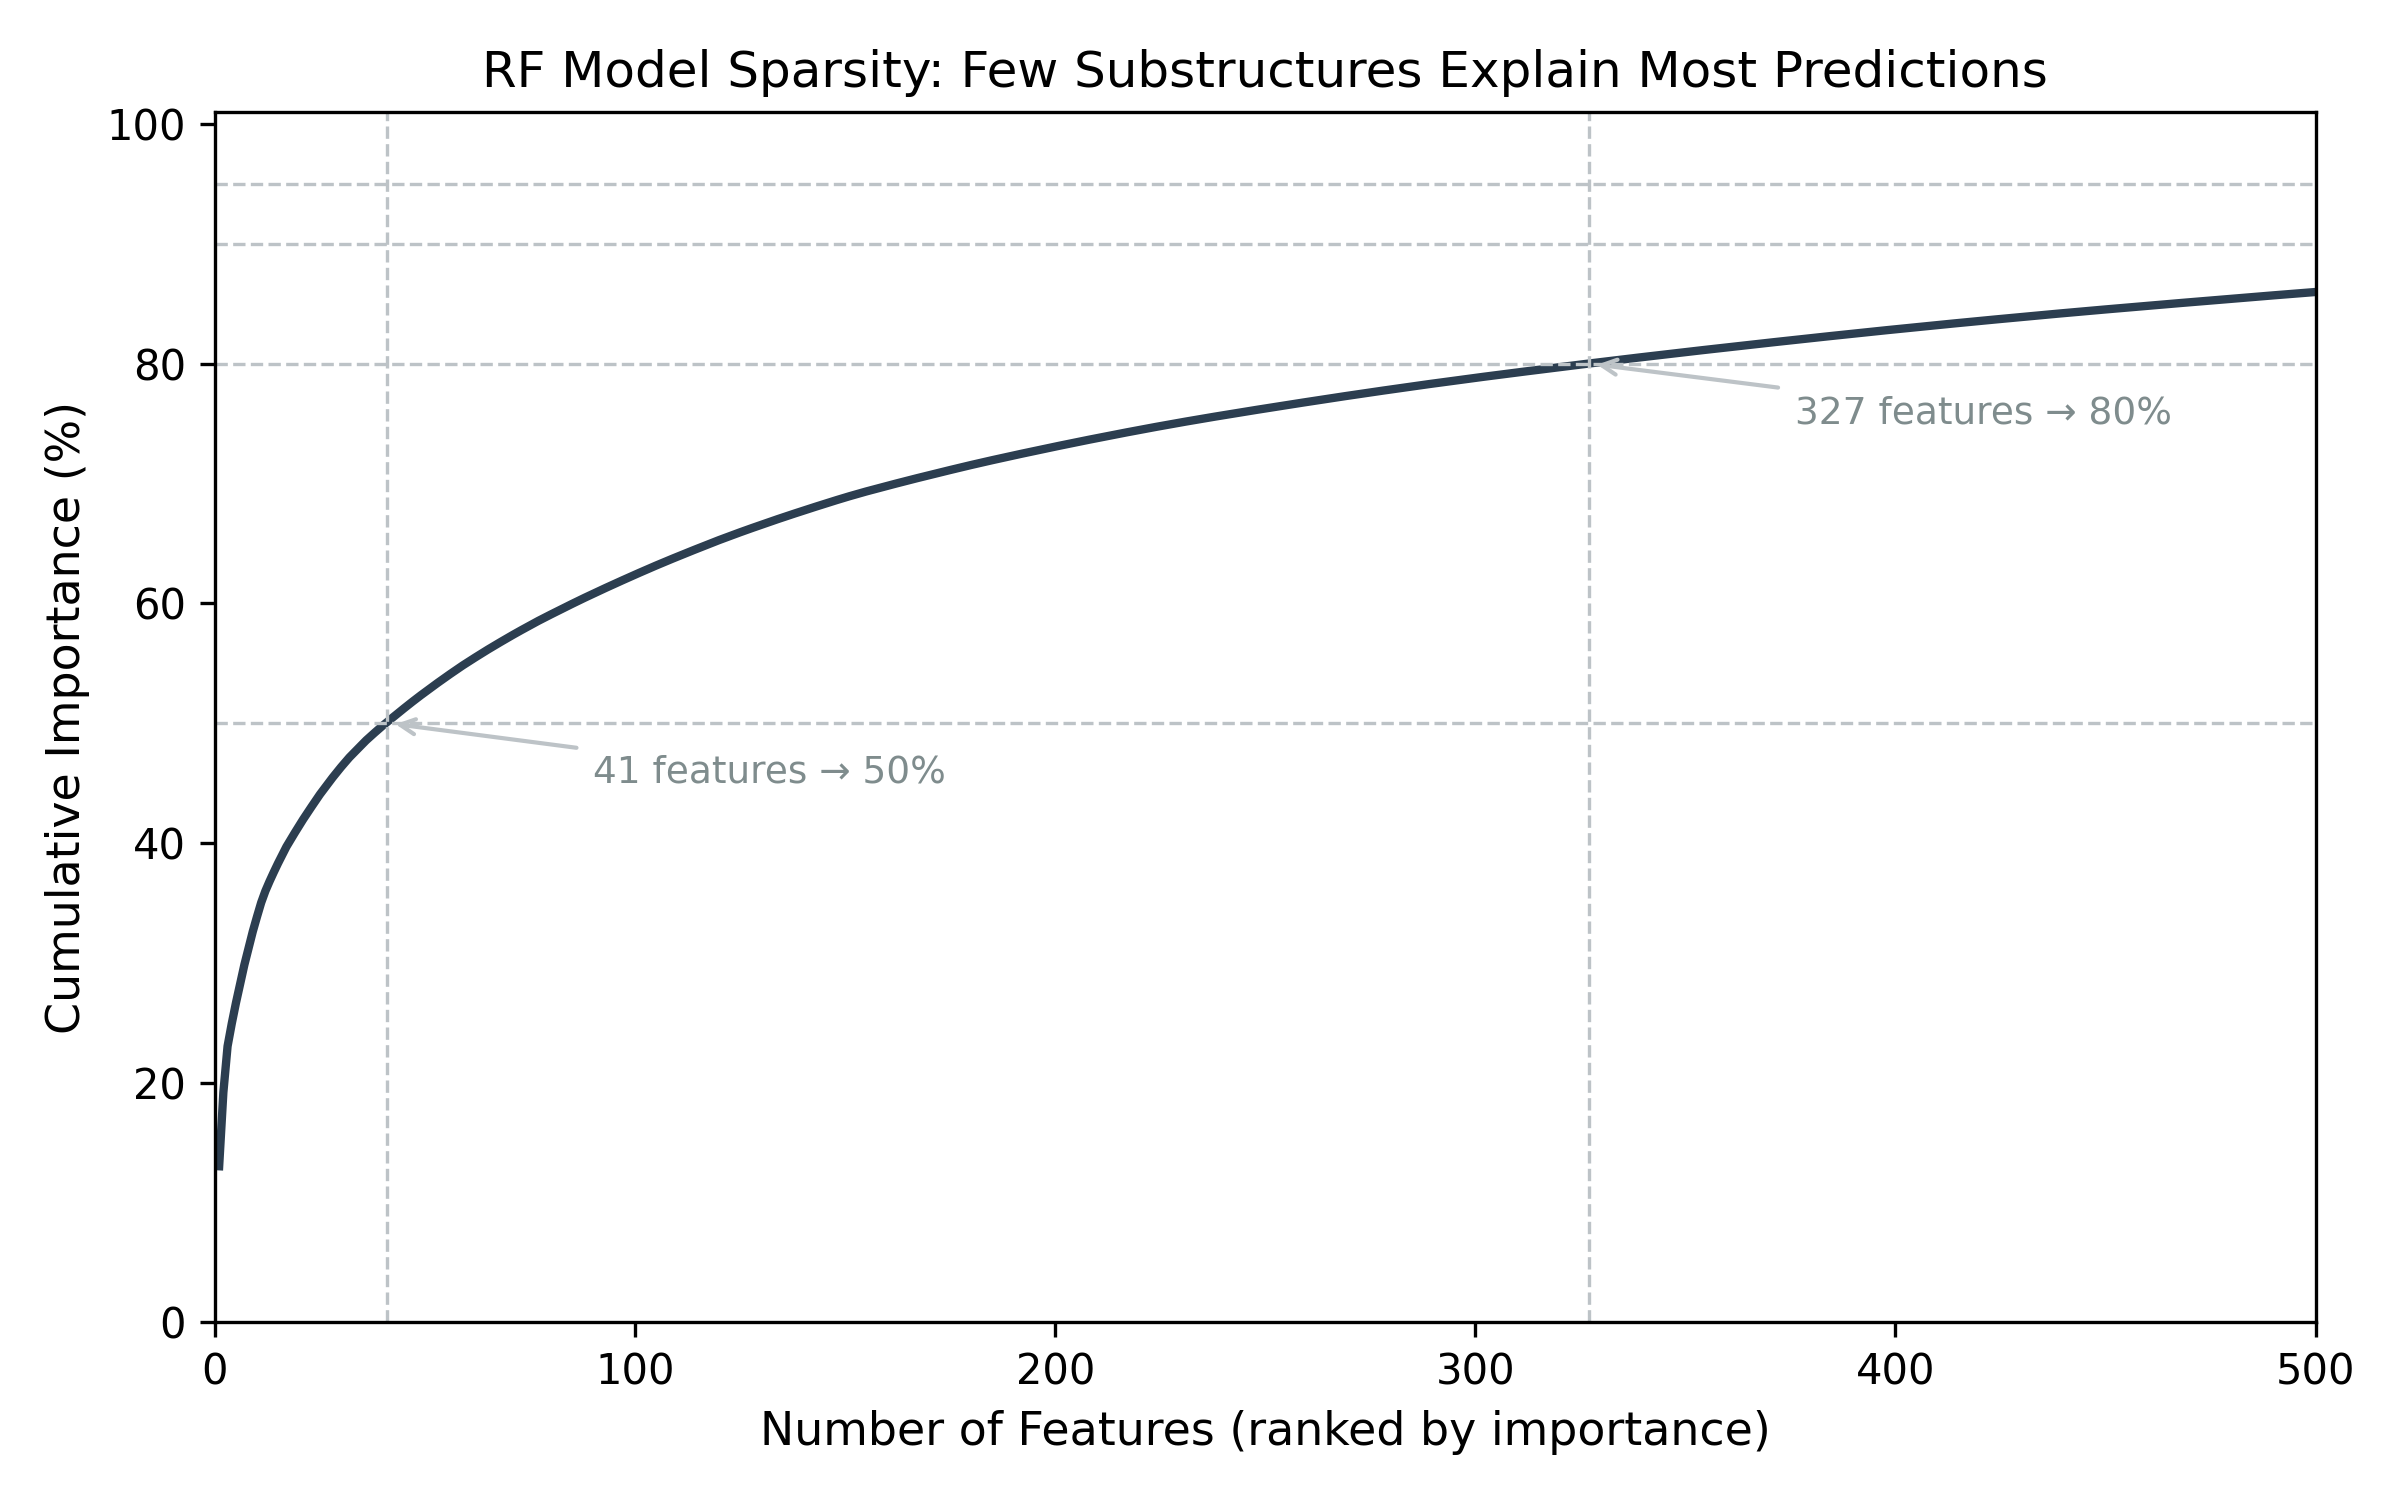
\includegraphics[width=0.65\textwidth]{results/rf_cumulative_importance.png}
    \caption{Cumulative feature importance. The top 41 features (out of 4096) account for 50\% of total importance, and 327 features reach 80\%, indicating a sparse, interpretable model.}
    \label{fig:rf_cumulative}
\end{figure}

\begin{figure}[htbp]
    \centering
    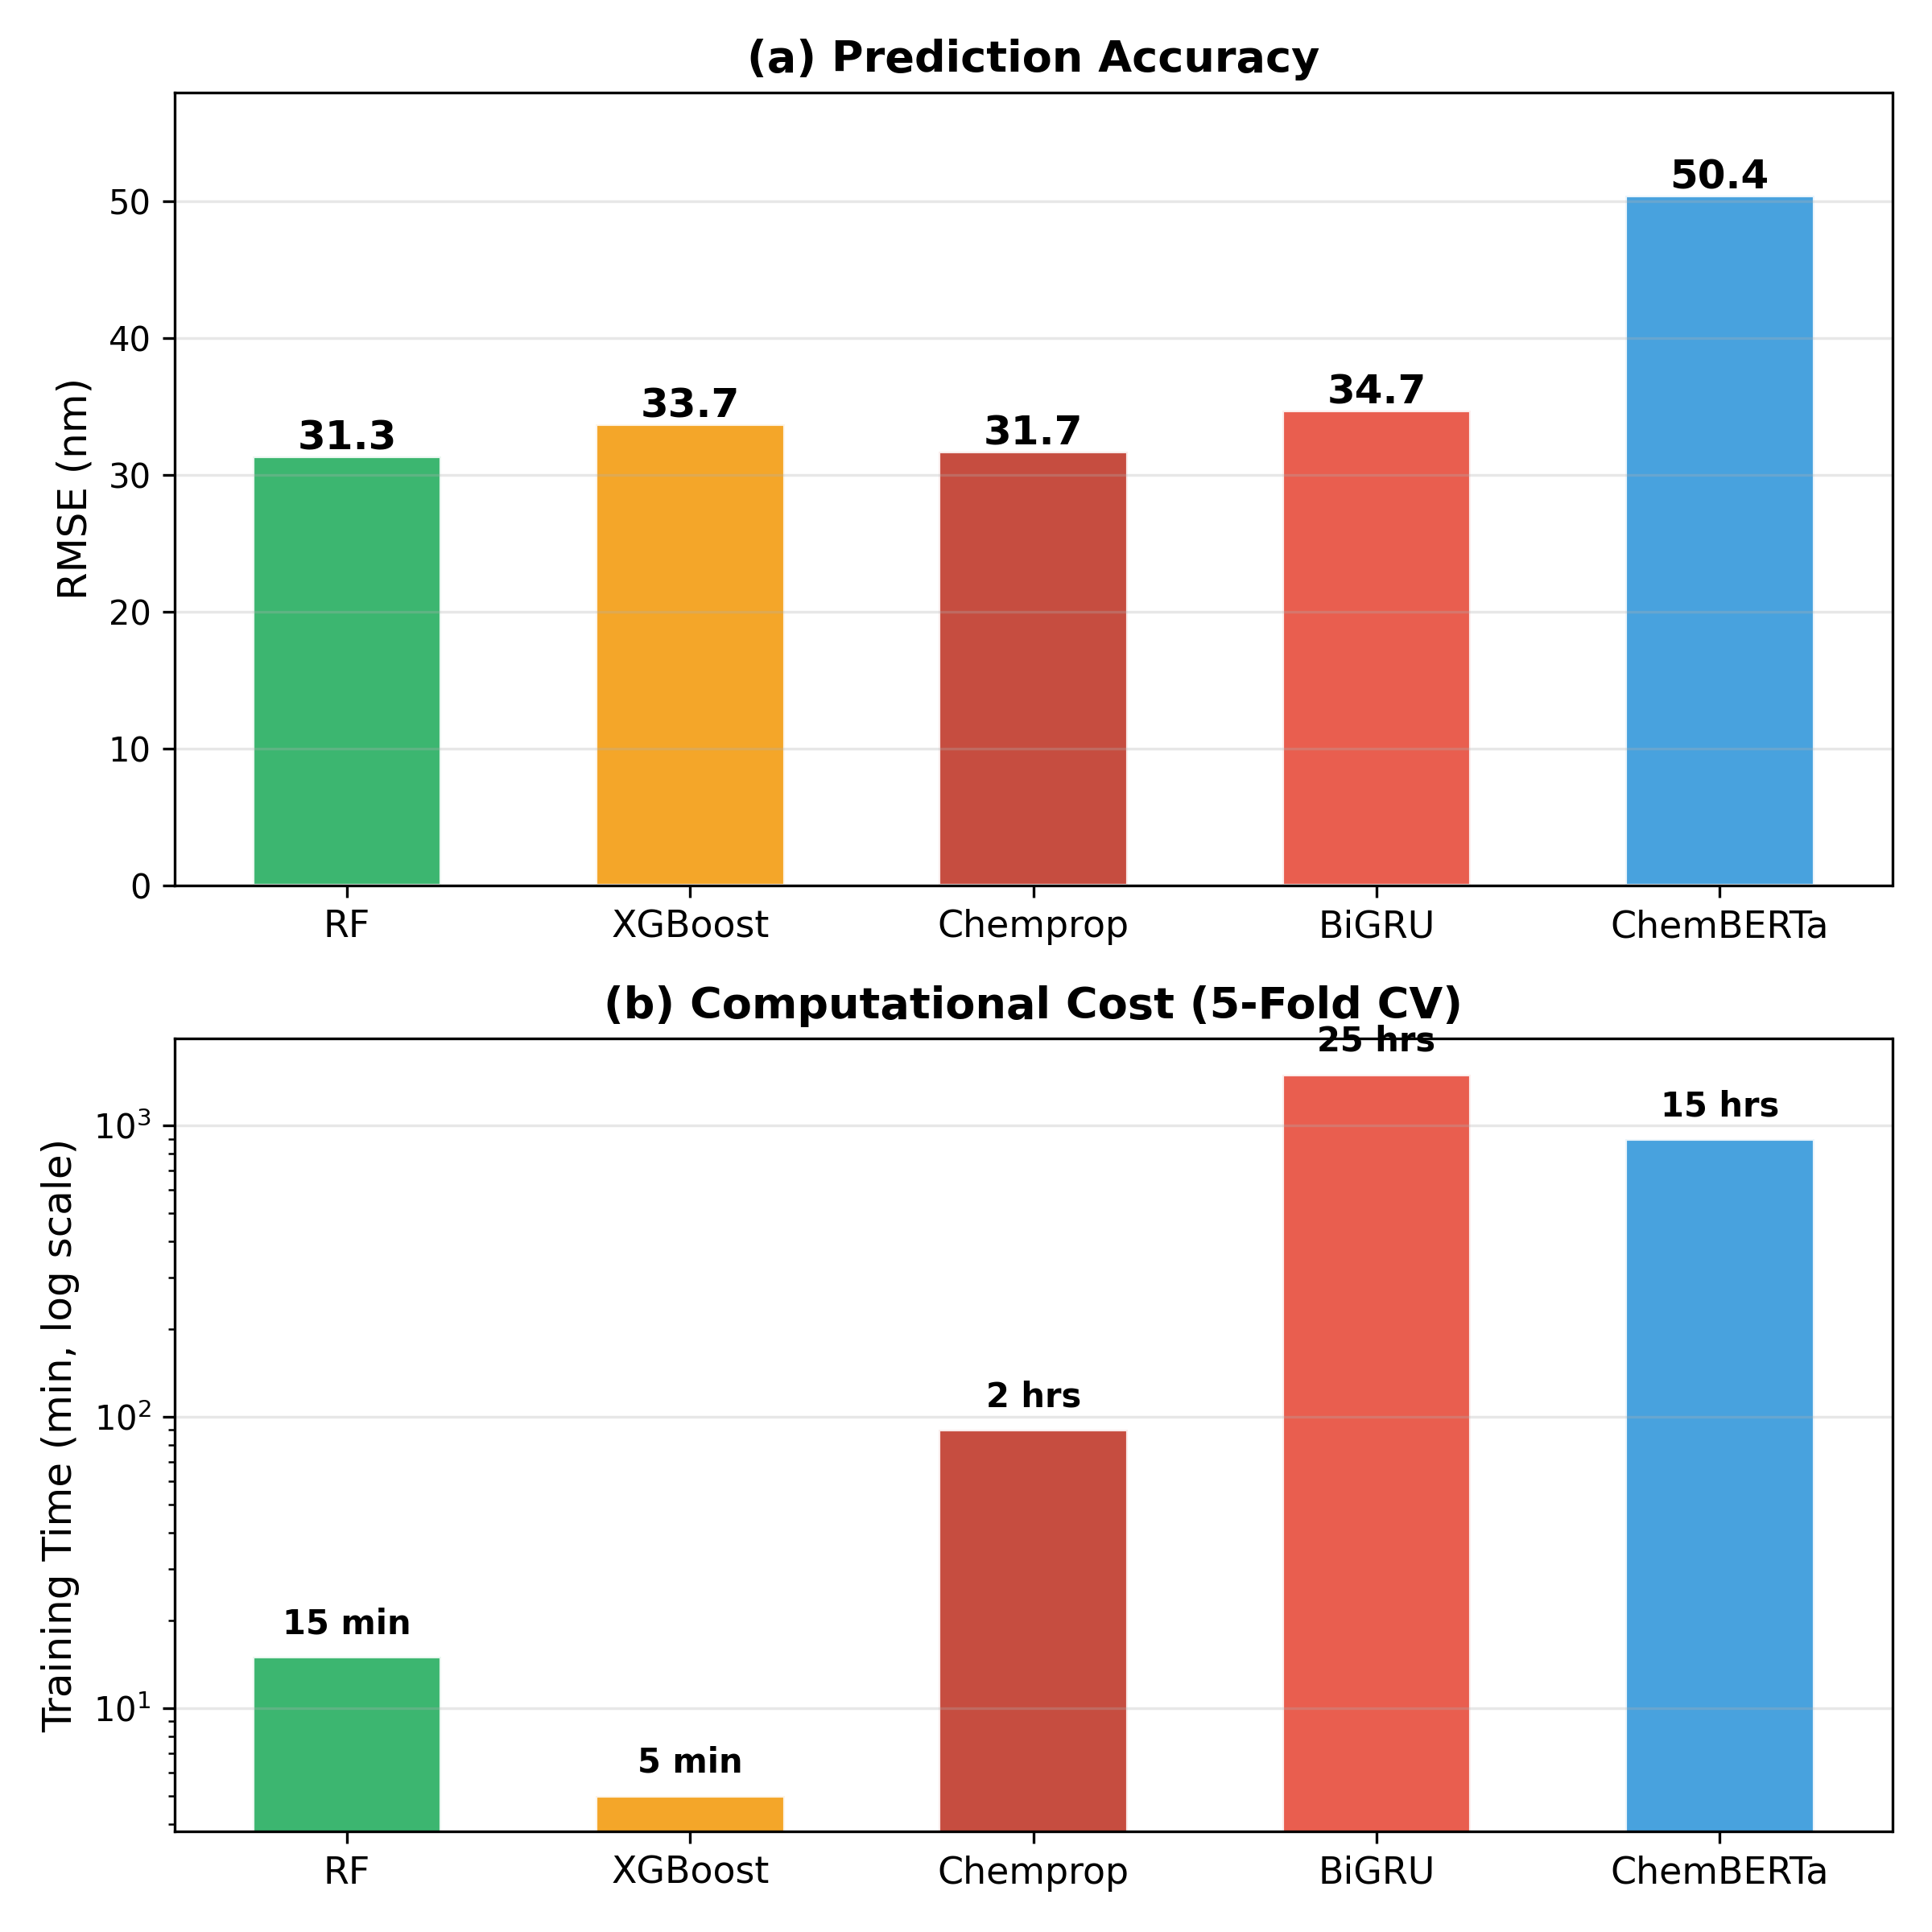
\includegraphics[width=0.65\textwidth]{results/rf_training_comparison.png}
    \caption{Training time vs.\ performance comparison. (a)~RF \removed{achieves the best RMSE}\added{attains performance statistically tied with the best deep learning model} in 15~minutes of total training compared to BiGRU's 25~hours (100$\times$ faster). (b)~Computational cost on log scale highlights the practical advantage of fingerprint-based models.}
    \label{fig:rf_practical}
\end{figure}

\textbf{Feature importance reveals known photochemistry.}
The most important feature (bit 463, Gini importance = 12.7\%) corresponds to aryl diazo/hydrazine substructures.
Molecules containing this substructure exhibit a mean $\lambda_{\max}$ of 543~nm compared to 401~nm without ($\Delta\lambda_{\max} = +143$~nm), consistent with the well-known bathochromic effect of nitrogen-nitrogen double bonds extending $\pi$-conjugation.
Other high-ranking features include BODIPY cores ($\Delta\lambda_{\max} = +162$~nm), enamine linkages ($\Delta\lambda_{\max} = +141$~nm), and alkynyl silane groups ($\Delta\lambda_{\max} = +153$~nm), all recognized chromophore motifs in photochemistry (Figure~\ref{fig:rf_interpretability}a).

\textbf{Solute dominates, solvent contributes modestly.}
Partitioning feature importance between solute and solvent fingerprint bits reveals that solute structure accounts for 96.1\% of total importance, with solvent contributing 3.9\% (Figure~\ref{fig:rf_interpretability}b).
This aligns with chemical intuition: chromophore structure is the primary determinant of $\lambda_{\max}$, while solvatochromic shifts are secondary effects.
The 24.6:1 solute-to-solvent importance ratio is consistent with the modest 6--8\% RMSE improvement observed in the solvent ablation.

\textbf{Model sparsity.}
Despite operating on 4096-dimensional fingerprint input, the RF model concentrates its decisions on a small subset of features: the top 5 features explain 26.9\% of total importance, the top 20 explain 41.6\%, and the top 100 explain 62.6\% (Figure~\ref{fig:rf_cumulative}).
A single fingerprint bit corresponding to aryl diazo/hydrazine substructures accounts for 12.7\% of total importance, reflecting the dominant contribution of azo chromophores to large $\lambda_{\max}$ values in the dataset ($\Delta\lambda = +143$~nm when present).

\textbf{Practical advantages of classical ML.}
Beyond interpretability, RF offers substantial practical advantages for molecular property prediction tasks.
RF training completes in approximately 15 minutes on a single CPU, compared to 1.5 hours for Chemprop and 25 hours for BiGRU on GPU, while achieving comparable or lower RMSE (Figure~\ref{fig:rf_practical}b).
RF requires no GPU hardware, no hyperparameter tuning of learning rates or batch sizes, and no early stopping strategy.
These results highlight that, depending on the dataset and molecular application domain, it is prudent to evaluate classical ML models where appropriate to gain insights into relative performance before directly deploying deep learning architectures.
While deep learning retains clear advantages in scenarios requiring transfer learning, end-to-end learning from raw data, or scalability to very large datasets, the simplicity, speed, and interpretability of fingerprint-based models make them a valuable complement, and in some cases a preferred alternative, in the molecular property prediction toolkit.

\textbf{Instance-level interpretability for BiGRU.}
While RF provides \emph{global} interpretability (which substructures matter dataset-wide), the BiGRU model offers complementary \emph{instance-level} interpretability.
Prior work has explored masking-based approaches for SMILES interpretability~\cite{gohSMILES2VecInterpretableGeneralPurpose2018}; here we explore gradient-based saliency analysis~\cite{simonyan2014deep}.
We computed Input$\times$Gradient saliency for each SMILES character position, then mapped character-level scores to atoms using RDKit's canonical SMILES atom-ordering~\cite{landrumRdkitRdkit2020_03_12020}, and visualized the resulting atom-level importance as 2D molecular heatmaps via SimilarityMaps~\cite{riniker2013similarity} (Figure~\ref{fig:bigru_saliency}).

The saliency maps reveal that BiGRU learns chemically meaningful patterns consistent with the RF feature importance analysis: high-saliency atoms concentrate on heteroatoms (O, N, S) and atoms adjacent to double bonds, the functional groups that determine $\pi$-conjugation and UV absorption wavelength, while aliphatic chains receive low saliency.
For molecules where BiGRU predicts accurately (e.g., Sinapic Acid, err = $-5.6$~nm), saliency is focused on the hydroxyl and methoxy groups of the chromophore; for poorly predicted molecules (e.g., Cinnamic Acid, err = $+78.2$~nm), the model over-attributes importance to the carboxylic acid rather than the conjugated vinyl bridge.
This convergence between RF's substructure-level Gini importance and BiGRU's atom-level gradient saliency provides independent confirmation that both models learn the same underlying photochemistry through fundamentally different architectures, a form of \emph{triangulation} that strengthens confidence in the learned structure--property relationships.
We note that gradient saliency identifies correlations rather than causal mechanisms, and that attention weights in Transformer-based models are even less reliable for interpretability~\cite{jain2019attention} (see Supporting Information, Figure~\removed{S3}\added{S5}, for character-type importance analysis).

\begin{figure}[htbp]
    \centering
    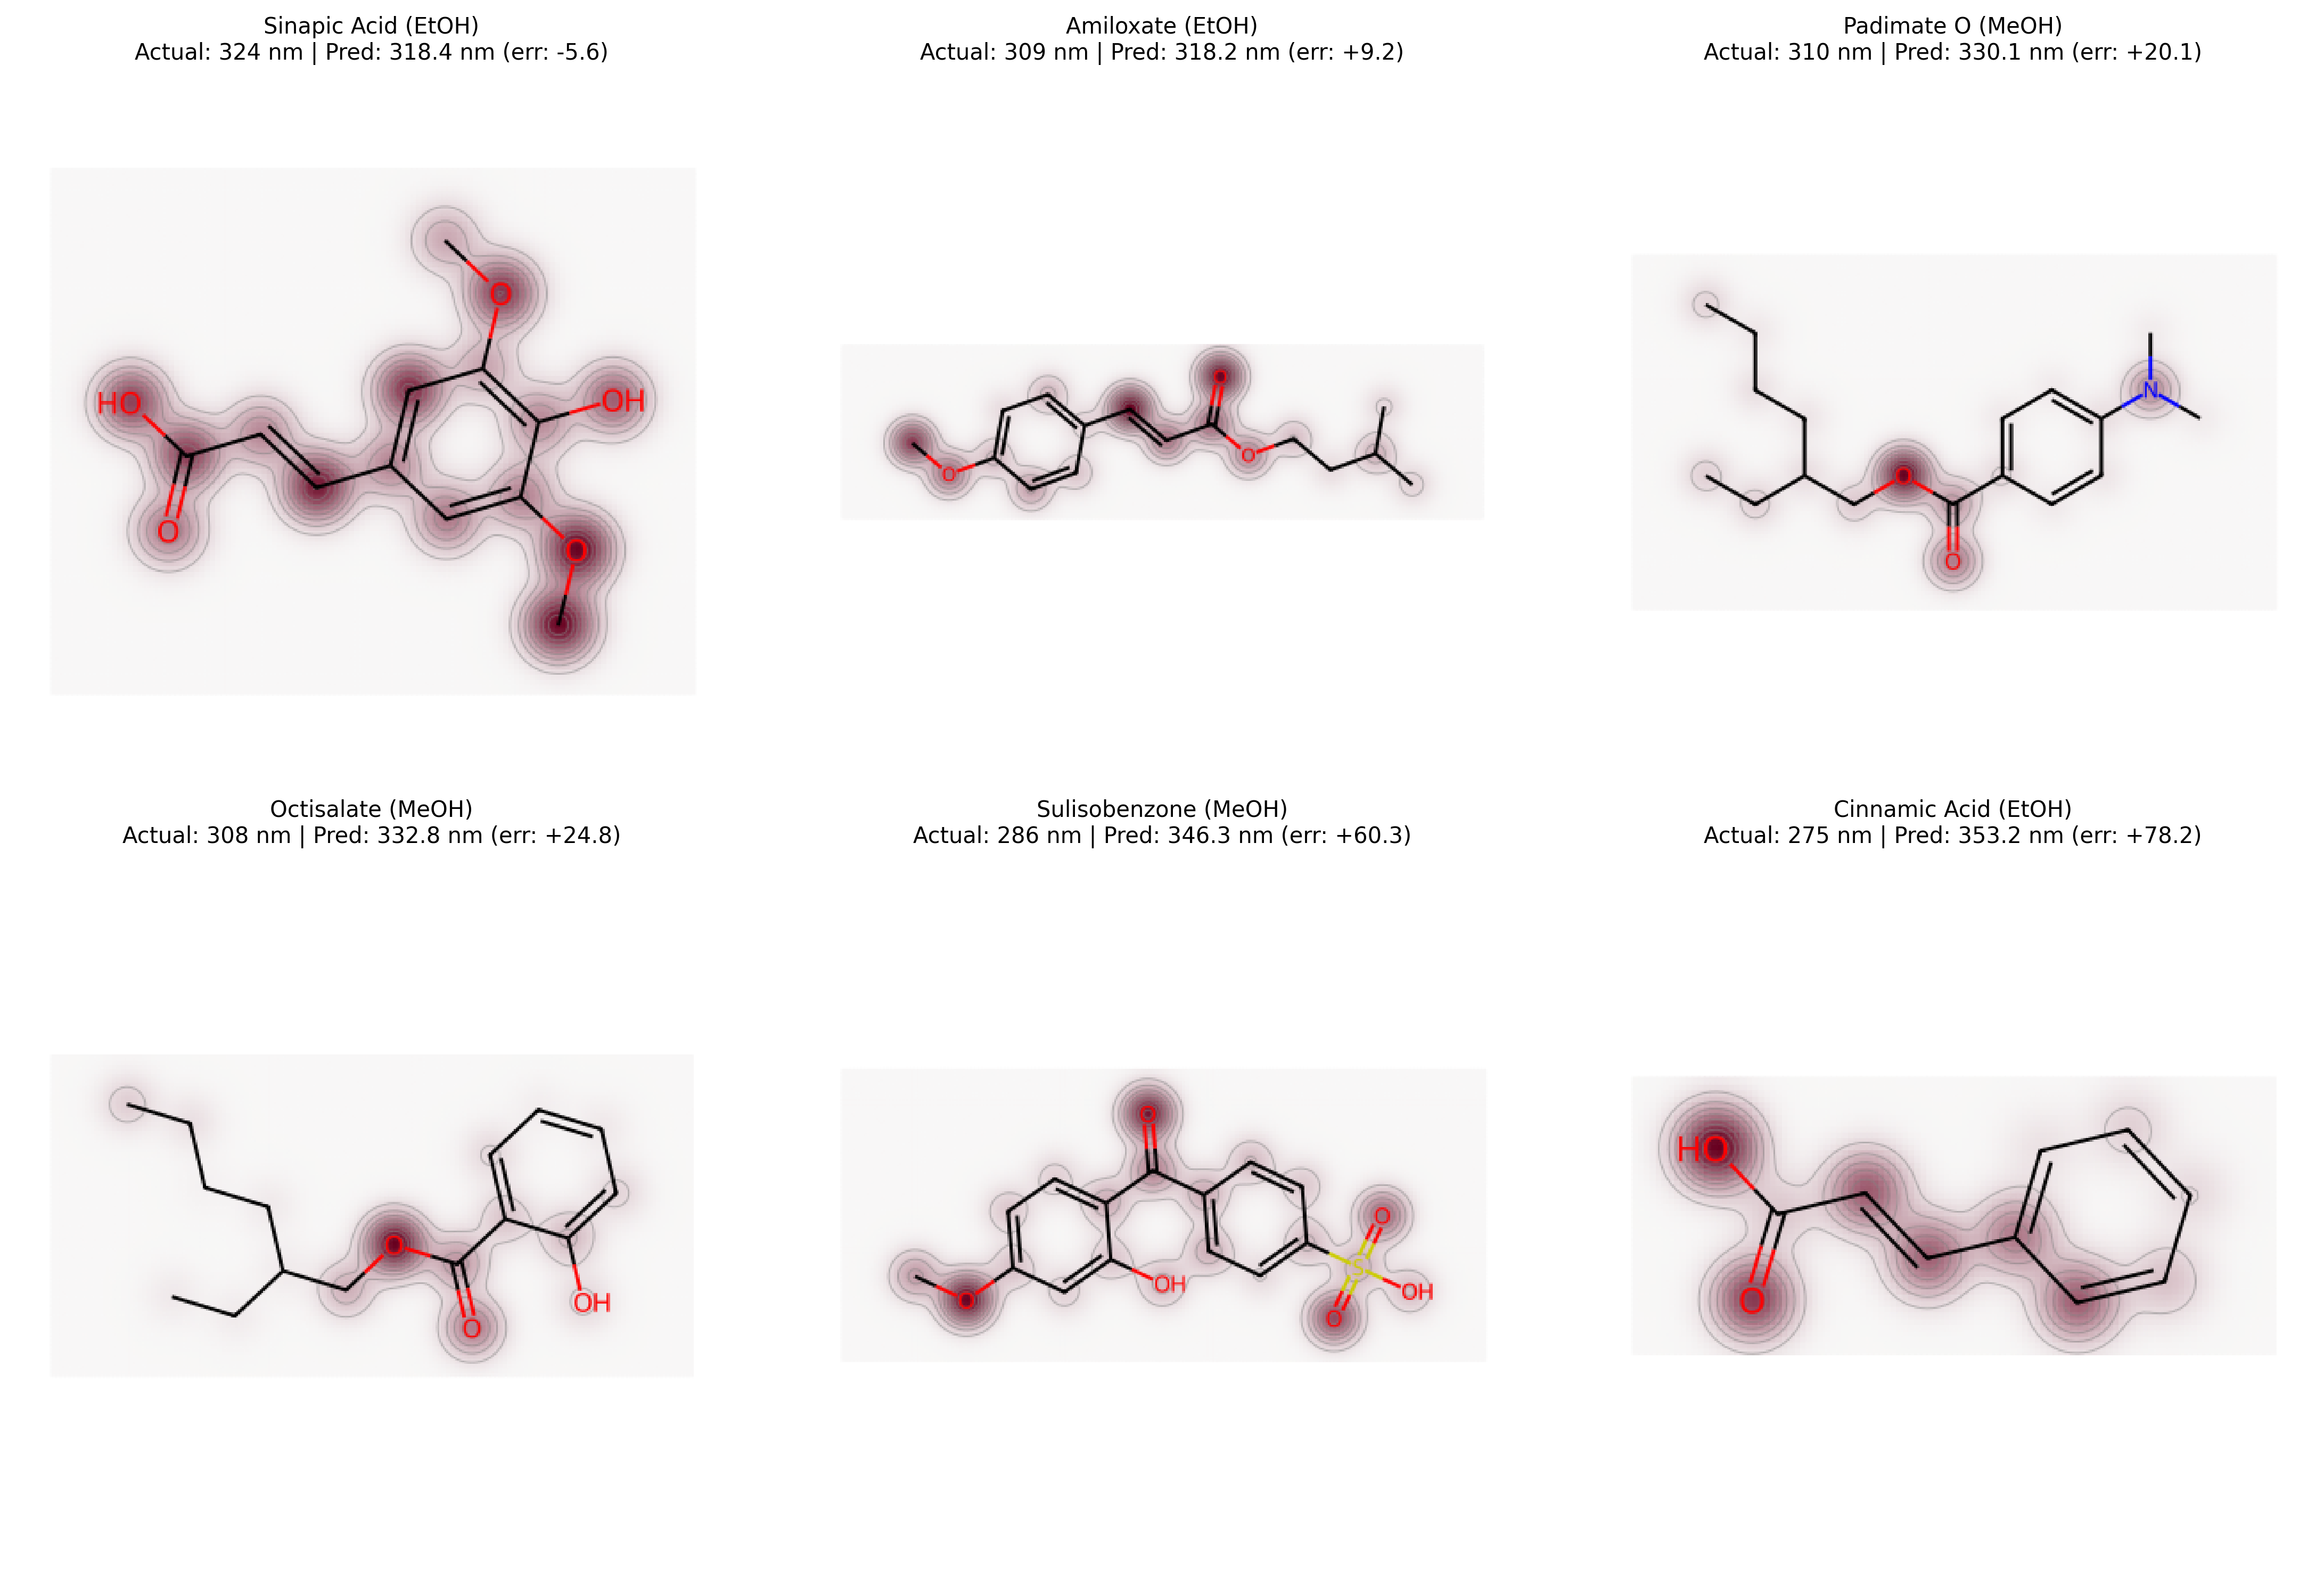
\includegraphics[width=\textwidth]{results/bigru_saliency_atoms.png}
    \caption{BiGRU gradient saliency mapped to 2D molecular structures for six wetlab validation molecules. Atom color intensity reflects gradient-based importance (red = high saliency). Top row: well-predicted molecules ($|\text{error}| < 22$~nm); bottom row: poorly predicted molecules ($|\text{error}| > 28$~nm). In both groups, heteroatoms (O, N) and atoms adjacent to double bonds receive the highest saliency, consistent with the character-type analysis (Figure~\removed{S3}\added{S5}) where bond symbols (\texttt{=}, \texttt{\#}) and heteroatoms rank $2.5\text{--}3.5\times$ above aliphatic carbons. This overlap with the chromophore motifs identified by RF feature importance confirms that the BiGRU learns chemically meaningful attention patterns. Large prediction errors (e.g., Octocrylene +61~nm, Cinnamic Acid +81~nm) therefore arise not from misidentified features but from limitations in encoding extended conjugation length and specific solvent effects from 1D SMILES.}
    \label{fig:bigru_saliency}
\end{figure}


% --- Photosafety Classification ---
\subsection{Photosafety Classification}
\label{sec:classification}

To evaluate practical utility, we apply our models to ICH~S10~\cite{ICH2013S10} photosafety classification using the Mamede et al.~\cite{mamede2021machine} protocol.
Compounds with $\lambda_{\max} \in [290, 700]$~nm and molar extinction coefficient (MEC) $\geq 1000$ are classified as photoreactive (POS).
\removed{We reconstructed the Mamede/Reaxys dataset by querying Reaxys using the CAS registry numbers listed in the original study, recovering 93.6\% of the original 74,784 compounds.}
\removed{The 6.4\% gap arises from deprecated CAS entries, compounds removed from current Reaxys builds, and structures that could not be resolved to valid SMILES representations.}
\added{We use the photosafety dataset from Mamede et al.~\cite{mamede2021machine}, who curated 74{,}784 compounds with binary photosafety labels (absorbance in 290--700~nm at MEC $\geq 1000$~L\,mol$^{-1}$\,cm$^{-1}$) from Reaxys. Rather than re-querying Reaxys (which requires institutional licensing), we use Mamede's published Supporting Information directly: a Reaxys-derived XRN+SMILES table provided in the original \emph{Scientific Reports} paper's SI. RDKit canonicalisation succeeds for 74{,}783 of the 74{,}784 entries (one SMILES fails to parse); the resulting 74{,}783-record dataset is used for the photosafety classification experiment described below. Full reproducibility pipeline (SI download URL, RDKit version, canonicalisation script, train/test split protocol) is given in Supporting Information Section~S16.}
We trained a separate RF classifier on this reconstructed data, and additionally trained the tuned BiGRU architecture (3-layer, 256-unit) as a direct binary classifier with sigmoid output and BCE loss on the same dataset and test split.

\begin{table}[htbp]
\centering
\caption{Photosafety classification performance. POS = $\lambda_{\max} \in [290,700]$ nm AND MEC $\geq$ 1000. $^\dagger$Published result on original Reaxys dataset; our models use a reconstructed version (93.6\% recovery) with a different test split, so comparison is approximate.}
\label{tab:classification}
\begin{tabular}{lccccc}
\toprule
\textbf{Model} & $\boldsymbol{N_{\text{test}}}$ & \textbf{Sensitivity} & \textbf{Specificity} & \textbf{Accuracy} & \textbf{AUC} \\
\midrule
Mamede RF (2021)$^\dagger$  & 998   & 0.90  & 0.88  & 0.89  & ---   \\
Our RF                      & 1,996 & 0.876 & 0.882 & 0.879 & 0.942 \\
BiGRU direct cls            & 1,996 & 0.794 & 0.811 & 0.803 & 0.886 \\
\bottomrule
\end{tabular}
\end{table}

Our RF classifier closely reproduces the published Mamede results (accuracy 0.879 vs.\ 0.89), validating both our Reaxys dataset reconstruction and the effectiveness of Morgan fingerprints for photosafety screening.
When the tuned BiGRU is trained as a direct binary classifier on the same data, it achieves accuracy 0.803, substantially below RF (0.879).
This gap reinforces the advantage of explicit substructure encoding (Morgan fingerprints) over character-level SMILES representations for classification tasks where specific functional-group presence determines the label.


% --- Experimental Validation ---
\subsection{Experimental Validation}
\label{sec:experimental}

To further validate our models, we measured UV absorption spectra for 16 commercially available compounds (Figure~\ref{fig:wetlab_molecules}) in both ethanol (EtOH) and methanol (MeOH), yielding 32 experimental $\lambda_{\max}$ values.
\removed{Of these 16 molecules, 15 are entirely absent from the training dataset, providing a genuine out-of-distribution test.}
\removed{One molecule (Ferulic Acid) appears in the training data with a different solvent (water).}
\added{At the SMILES level, only Ferulic Acid is an exact duplicate of a training record; the other 15 molecules are absent from the training data and are fingerprint-distant from it (nearest-neighbour Tanimoto similarity using Morgan radius-2/2048-bit fingerprints: mean~$= 0.58$, median~$= 0.58$, with 5/16 molecules below the $0.5$ ``dissimilar'' threshold and only the Ferulic-Acid duplicate above $0.7$). At the Bemis--Murcko scaffold level, however, 15/16 generic scaffolds are present in the v3 training set; only Avobenzone (a 1,3-diketone bridging two substituted phenyls) is scaffold-novel. The wetlab set therefore tests \emph{molecule-level} (novel substitution-pattern) generalisation on chromophore classes the models have seen at the scaffold level (the operational deployment scenario for the photosafety- and UV-filter-screening applications this manuscript targets) rather than full scaffold-class extrapolation. The per-molecule similarity table, the four-bin Tanimoto distribution, the scaffold-match counts, and a stricter Tanimoto-$\leq 0.5$ subset analysis (the five truly fingerprint-novel molecules, on which the DL-vs-RF gap actually \emph{widens}) are in Supporting Information Section~S14.}
Although ethanol and methanol are well-represented solvents in the training set (1,034 and 1,322 records, respectively), the solute--solvent combinations tested here are novel.

\begin{figure}[htbp]
\centering
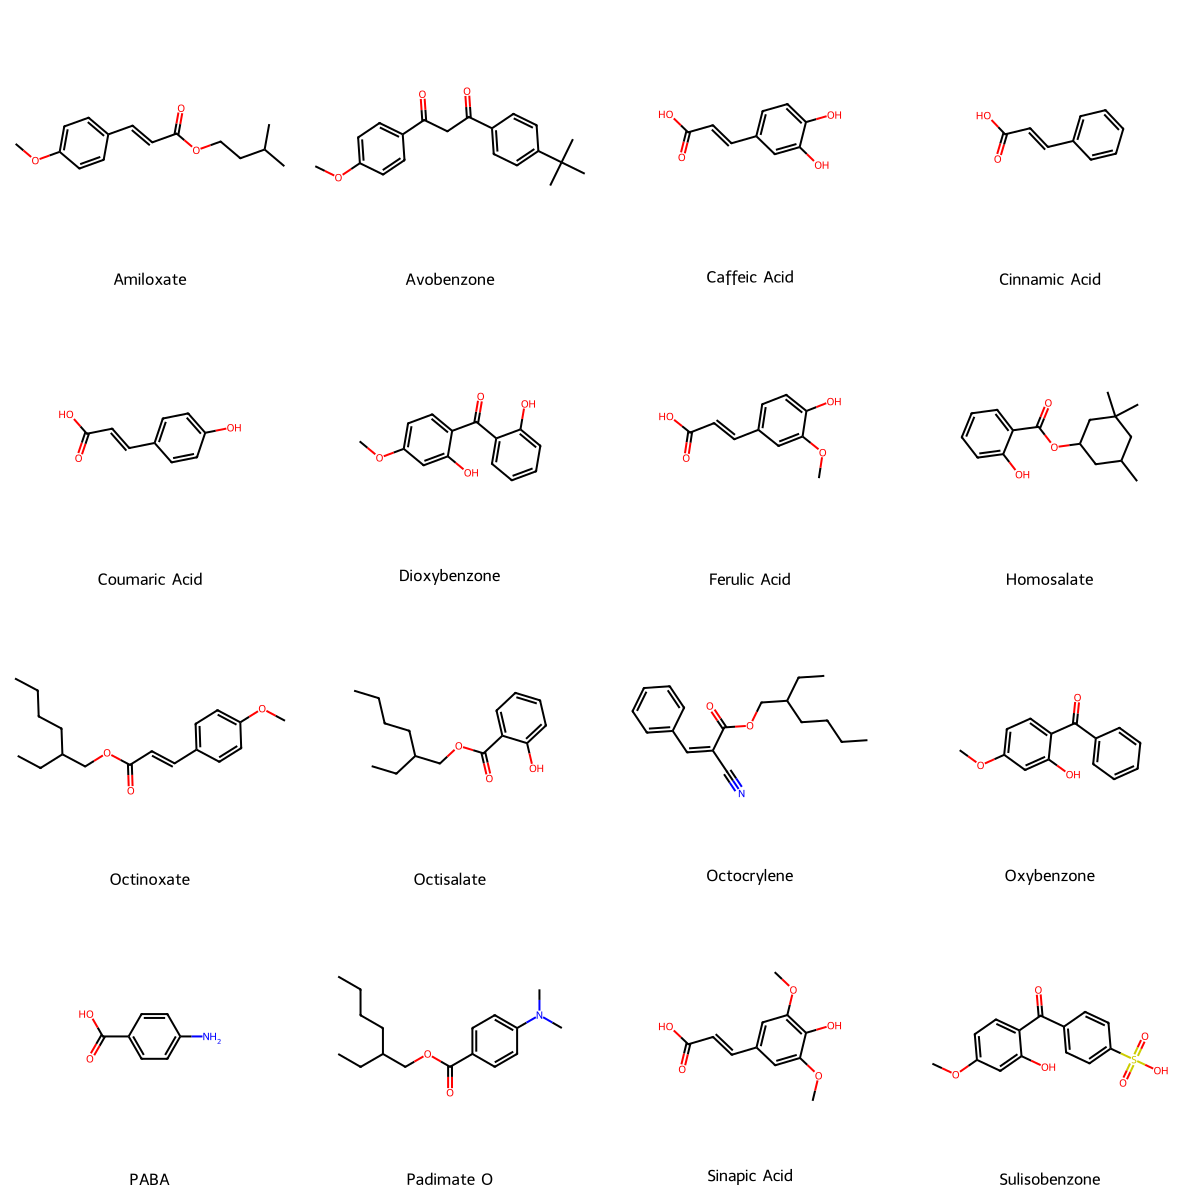
\includegraphics[width=\columnwidth]{results/wetlab_molecules.png}
\caption{Molecular structures of the 16 UV-absorbing compounds used for experimental validation. These commercially available sunscreen actives and phenolic acids span a range of chromophore classes (cinnamates, salicylates, benzophenones, aminobenzoates) with experimental $\lambda_{\max}$ values from 275 to 358~nm.}
\label{fig:wetlab_molecules}
\end{figure}

\begin{table}[htbp]
\centering
\caption{Experimental validation: predicted vs.\ measured $\lambda_{\max}$ (nm) for 16 UV-absorbing compounds in two solvents. GNN = D-MPNN, CB = ChemBERTa. Predictions are ensemble averages across 5-fold models. \colorbox{goodpred}{Green} cells indicate predictions within 10~nm of the experimental value. $^*$Present in training data with a different solvent.}
\label{tab:experimental}
\small
\begin{tabular}{lccccccccccc}
\toprule
& \multicolumn{5}{c}{\textbf{Ethanol}} & & \multicolumn{5}{c}{\textbf{Methanol}} \\
\cmidrule(lr){2-6} \cmidrule(lr){8-12}
\textbf{Molecule} & \textbf{Exp.} & \textbf{GNN} & \textbf{CB} & \textbf{BiGRU} & \textbf{RF} & & \textbf{Exp.} & \textbf{GNN} & \textbf{CB} & \textbf{BiGRU} & \textbf{RF} \\
\midrule
Amiloxate       & 309 & \gp{309} & 349 & \gp{318} & 359 & & 298 & \gp{302} & 347 & 316 & 359 \\
Avobenzone      & 358 & \gp{354} & 323 & 329 & 337 & & 358 & \gp{351} & 318 & 327 & 333 \\
Caffeic Acid    & 325 & \gp{319} & 342 & 338 & 347 & & 325 & 309 & \gp{335} & \gp{335} & 345 \\
Cinnamic Acid   & 275 & \gp{276} & 348 & 353 & 348 & & 276 & 265 & 341 & 351 & 345 \\
Coumaric Acid   & 310 & \gp{302} & 340 & 348 & 346 & & 309 & 294 & 333 & 343 & 344 \\
Dioxybenzone    & 283 & 367 & 314 & 315 & 327 & & 283 & 359 & 308 & 315 & 320 \\
Ferulic Acid$^*$  & 324 & 311 & \gp{326} & 313 & 346 & & 324 & 302 & \gp{321} & 310 & 344 \\
Homosalate      & 308 & 336 & 295 & 335 & 332 & & 308 & 335 & 293 & 336 & 327 \\
Octinoxate      & 309 & 328 & 325 & 326 & 334 & & 308 & 322 & 323 & 323 & 332 \\
Octisalate      & 308 & 334 & 291 & 339 & 353 & & 308 & 333 & 291 & 333 & 349 \\
Octocrylene     & 301 & 385 & 357 & 344 & 390 & & 302 & 381 & 350 & 344 & 389 \\
Oxybenzone      & 287 & 334 & 325 & \gp{301} & 328 & & 287 & 327 & 317 & \gp{299} & 321 \\
PABA            & 291 & \gp{282} & \gp{295} & 322 & 308 & & 290 & 279 & \gp{294} & 319 & 306 \\
Padimate O      & 310 & 325 & \gp{320} & 334 & 340 & & 310 & 324 & \gp{316} & 330 & 337 \\
Sinapic Acid    & 324 & 312 & 343 & \gp{318} & 347 & & 324 & 303 & \gp{332} & \gp{314} & 346 \\
Sulisobenzone   & 287 & 338 & 330 & 346 & 355 & & 286 & 334 & 326 & 346 & 352 \\
\midrule
\textbf{MAE (nm)} & & \textbf{25.5} & 27.8 & 28.9 & 39.3 & & & \textbf{26.9} & 24.9 & 28.4 & 37.7 \\
\textbf{RMSE (nm)} & & 36.5 & \textbf{33.5} & 34.4 & 44.4 & & & 34.8 & \textbf{30.8} & 33.4 & 43.0 \\
\bottomrule
\end{tabular}
\end{table}

\begin{table}[htbp]
\centering
\caption{Aggregate wetlab validation metrics (16 molecules $\times$ 2 solvents = 32 data points). 95\% bootstrap CIs from 10,000 resamples.}
\label{tab:wetlab_summary}
\begin{tabular}{lcc}
\toprule
\textbf{Model} & \textbf{MAE (nm) [95\% CI]} & \textbf{RMSE (nm) [95\% CI]} \\
\midrule
Chemprop (D-MPNN) & \textbf{26.2}              & 35.7 \\
ChemBERTa         & 26.3 [20.1--33.0] & \textbf{32.2} [25.2--38.8] \\
BiGRU (default)   & 28.6 [22.7--35.0] & 33.9 [26.2--41.2] \\
BiGRU (tuned)     & 31.5 & 37.0 \\
RF + Morgan FP    & 38.5 [31.6--45.9]          & 43.7 [35.3--51.7] \\
\bottomrule
\end{tabular}
\end{table}

Chemprop (GNN), ChemBERTa (CB-Transformer), and BiGRU all outperform RF on this experimental validation set. Averaging across both solvents (32 predictions), Chemprop achieves the lowest MAE (26.2~nm), followed closely by ChemBERTa (26.3~nm [95\% bootstrap CI: 20.1--33.0]), BiGRU (28.6~nm [22.7--35.0]), and RF (38.5~nm [31.6--45.9]).
ChemBERTa achieves the lowest RMSE (32.2~nm) because Chemprop has several large outlier errors on benzophenone derivatives (Dioxybenzone, Oxybenzone: 40--84~nm errors), inflating its RMSE (35.7~nm) despite competitive median accuracy.
On cross-validated benchmarks, ChemBERTa was worst (RMSE = \removed{50.39}\added{54.09~nm on v3, 50.39}~nm) and Chemprop was tied with RF\added{ ($p = 0.16$ on v3)}; yet on novel compounds, deep learning models consistently outperform RF.
This gap reflects a fundamental difference: RF relies on exact substructure matching through Morgan fingerprint bits, excelling at interpolation within the training distribution but struggling when novel functional groups or conjugation patterns are underrepresented.
The deep learning models, by contrast, learn representations (Chemprop from molecular graphs, BiGRU from sequential SMILES patterns, ChemBERTa from pretrained molecular language understanding) that can generalize to unseen molecular motifs.
All models show substantially higher errors than their cross-validated performance (ChemBERTa: 26.3 vs.\ \removed{24.3}\added{26.8~nm MAE on v3; 24.3}~nm MAE; BiGRU default: 28.6 vs.\ 20.7~nm; RF: 38.5 vs.\ \removed{15.2}\added{15.4}~nm \added{on v3}), confirming that these 16 compounds are genuinely challenging out-of-distribution examples.
The tuned BiGRU (3L/256u) performs \textit{worse} on wetlab validation (MAE = 31.5~nm) than the default (28.6~nm), despite 4.8\% lower cross-validated RMSE. This is a bias--variance tradeoff: the larger architecture overfits to in-distribution patterns at the cost of out-of-distribution generalization.

Cinnamic Acid (experimental $\lambda_{\max}$ = 275--276~nm) is a notable outlier: ChemBERTa, BiGRU, and RF all overpredict by $\sim$65--78~nm, though Chemprop handles it well (1--11~nm error).
The experimental peak lies at the edge of the 270--400~nm scan range, suggesting measurement limitations.
Octocrylene is particularly problematic for RF (error $\sim$89~nm) and Chemprop ($\sim$81~nm), vs.\ 43~nm for BiGRU and 52~nm for ChemBERTa, likely because its extended cyano-acrylate conjugation is underrepresented in the training data.

All three models capture the small solvent sensitivity between EtOH and MeOH (typically 0--1~nm experimentally), though with some overestimation of the solvent shift magnitude (average predicted shifts of 2.5~nm for BiGRU, 2.9~nm for RF, and 4.9~nm for ChemBERTa).

These results show that RF is the preferred choice for screening within known chemical space (e.g., virtual screening of compound libraries with well-represented scaffolds), while deep learning models (BiGRU and ChemBERTa) are better suited for exploring novel molecular architectures where the training distribution may not cover all relevant substructures.
This data-dependent model selection finding is consistent with the observations of Chen et al.~\cite{chenMolecularLanguage2023}, who found that RNNs outperform Transformers on local-feature-dependent molecular generation tasks.
Our cross-validated results suggest that a similar architectural trade-off may apply in property prediction: since UV absorption depends on local chromophore features, models that capture local patterns (RF with fingerprints, BiGRU processing SMILES subsequences) achieve the best in-distribution performance.
ChemBERTa's weak cross-validated performance but strong wetlab generalization suggests that pretrained representations may encode transferable molecular knowledge that compensates for the architecture's inductive bias mismatch, but only when evaluated on truly novel compounds outside the training distribution.
This complementarity extends beyond the local/global distinction: RF's fixed-vocabulary substructure matching excels at interpolation, while learned representations (both BiGRU and ChemBERTa) enable extrapolation to novel scaffolds.

\begin{figure}[htbp]
    \centering
    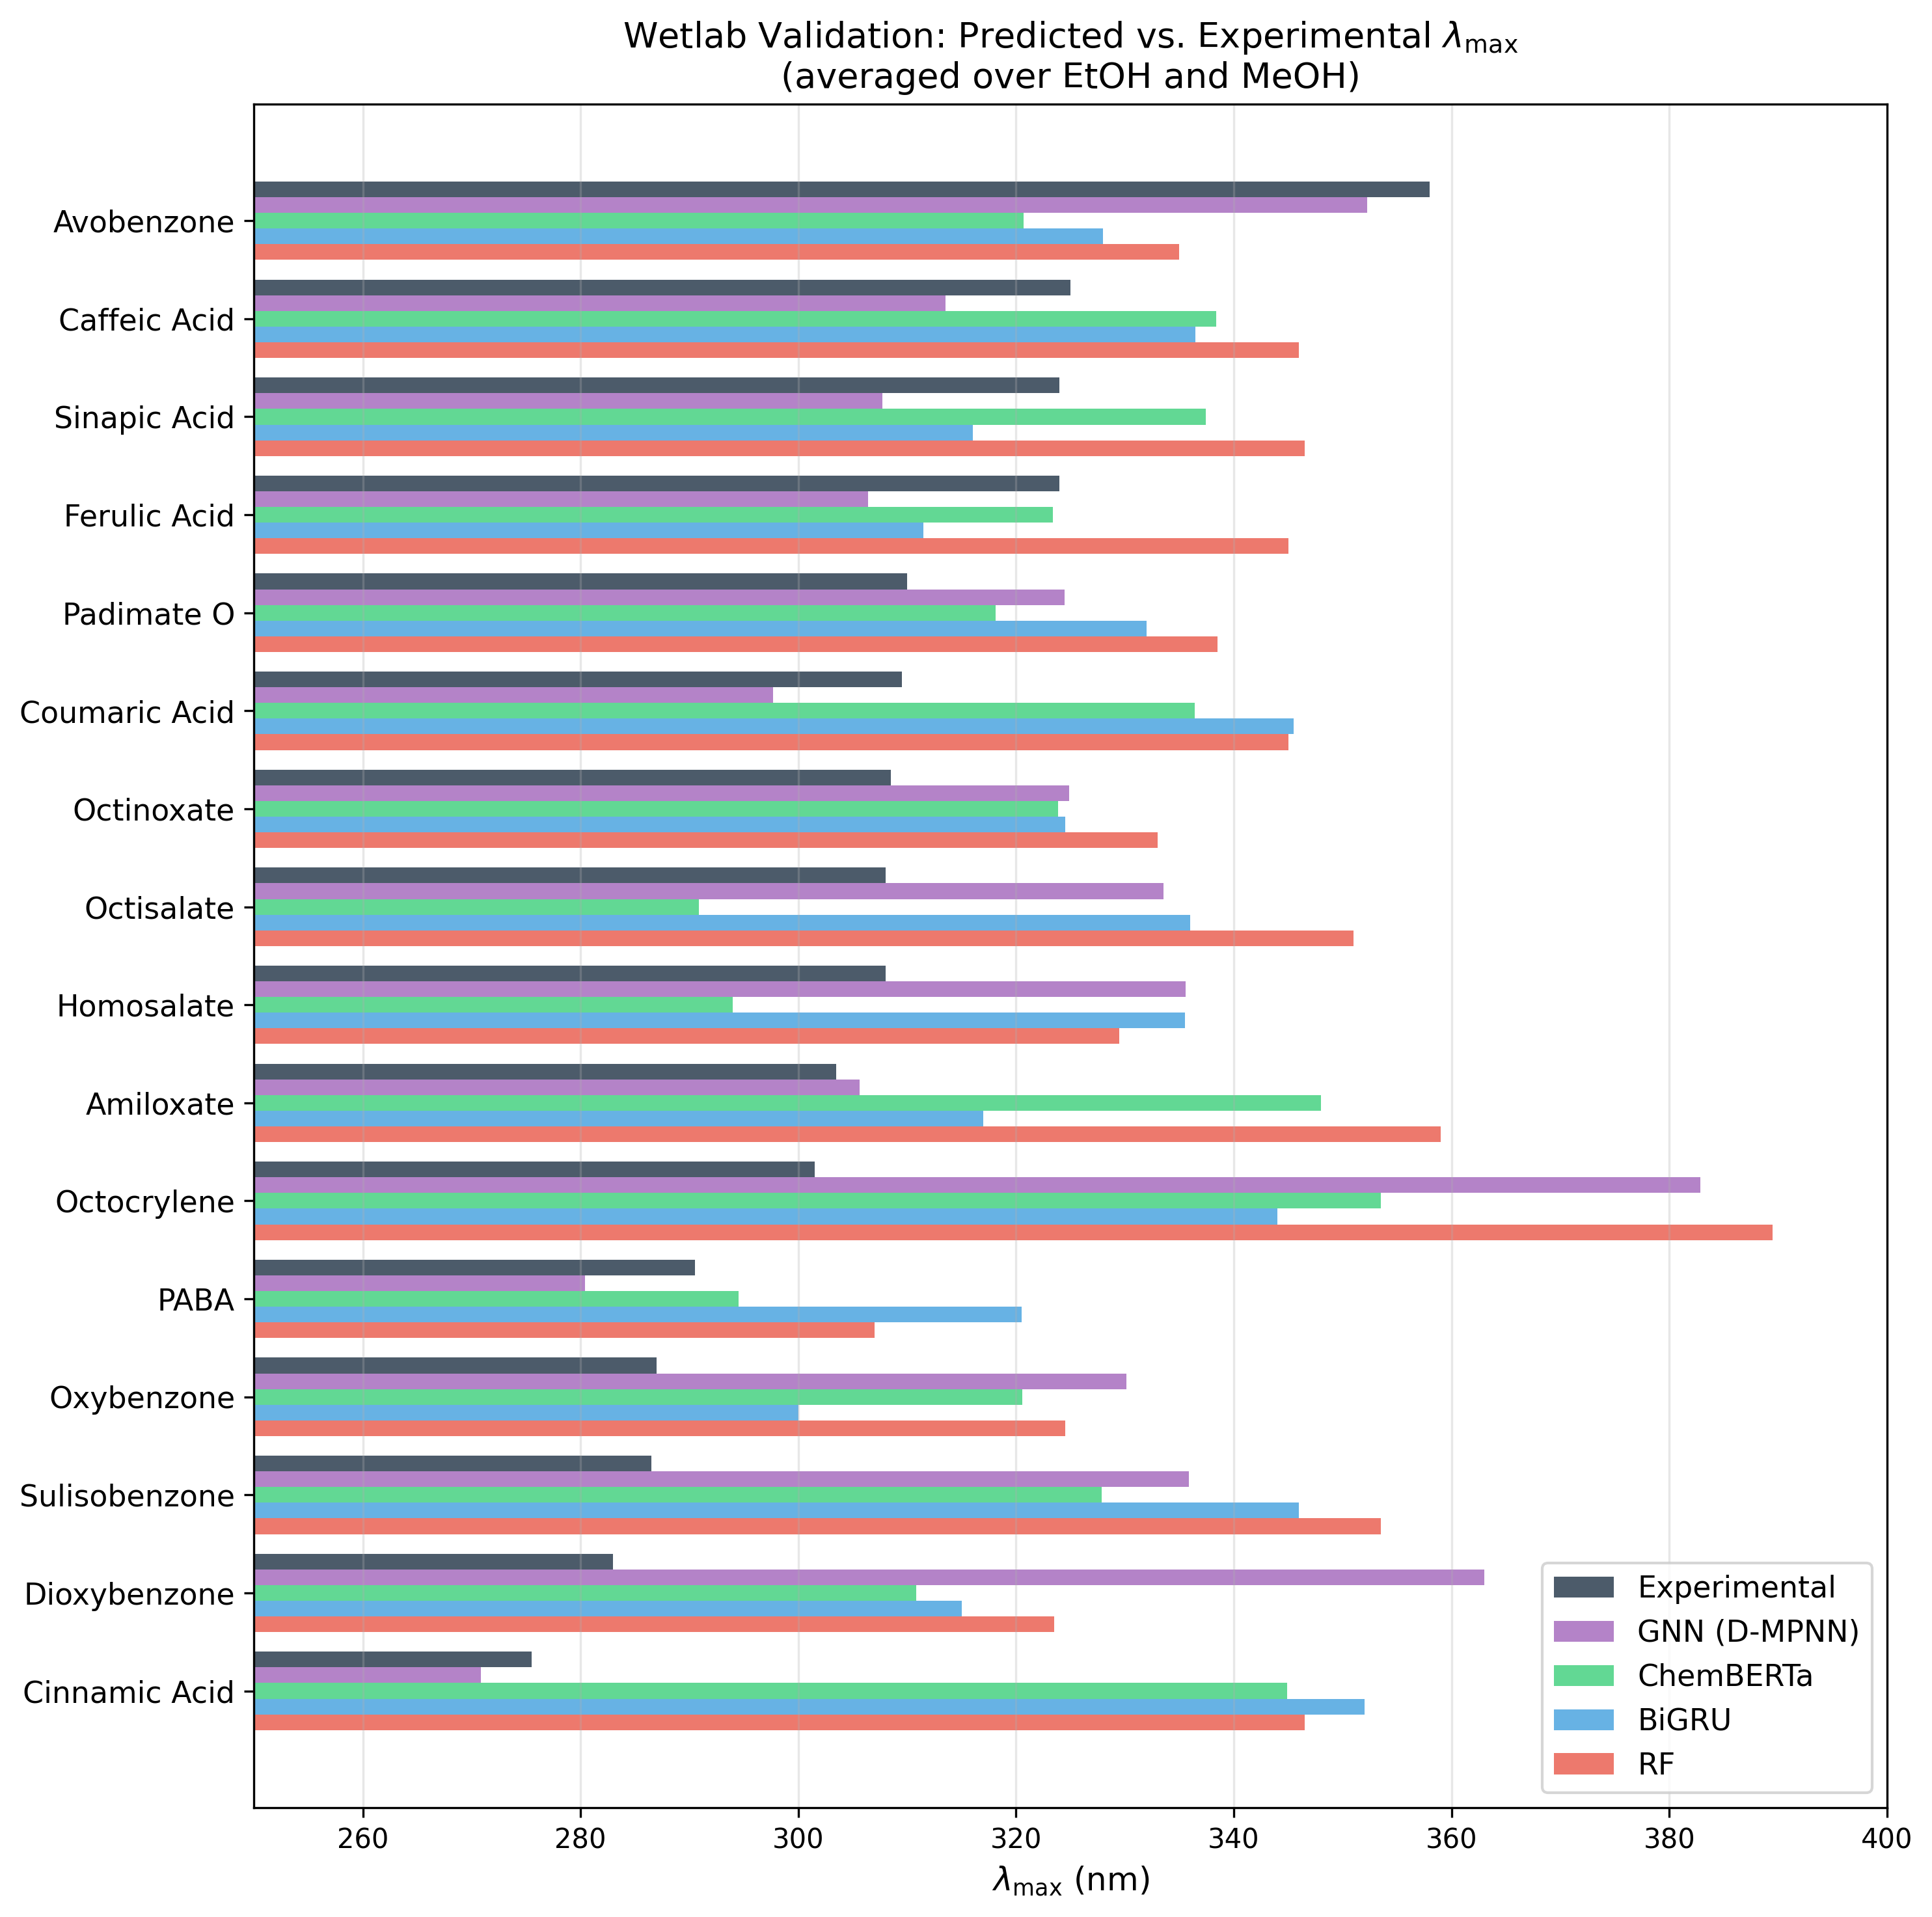
\includegraphics[width=\textwidth]{results/wetlab_per_molecule.png}
    \caption{Per-molecule comparison of experimental and predicted $\lambda_{\max}$ for 16 sunscreen-related compounds, averaged over EtOH and MeOH solvents. Molecules are sorted by experimental $\lambda_{\max}$. The D-MPNN closely tracks experimental values for small chromophores (Cinnamic Acid, PABA) but overpredicts benzophenones (Dioxybenzone, Octocrylene), while all models struggle with Octocrylene.}
    \label{fig:wetlab_per_molecule}
\end{figure}

Figure~\ref{fig:wetlab_per_molecule} shows per-molecule predictions alongside experimental values, illustrating the pattern more concretely: the D-MPNN achieves near-exact predictions for Cinnamic Acid and PABA where other models overpredict by 60--80~nm, while all models struggle with Octocrylene. ChemBERTa tracks the experimental trend most closely for mid-range absorbers (Padimate~O, Ferulic Acid).

% ===== Conclusion =====
\section{Conclusion}
\label{sec:conclusion}

We have presented a systematic benchmark of ML approaches for UV absorption wavelength prediction, comparing Random Forest, XGBoost, Chemprop (D-MPNN), BiGRU, and ChemBERTa across three datasets totaling over 60,000 molecules.

Our key findings are:

\begin{enumerate}
    \item \textbf{RF and deep learning have complementary strengths.}
    RF with Morgan fingerprints and the Chemprop D-MPNN achieve statistically indistinguishable cross-validated performance on the primary Joung+Beard \added{v3 cleaned }dataset (RMSE = \removed{31.34 and 31.69}\added{31.50 and 33.15}~nm, $p = \removed{0.77}\added{0.16}$\added{, see Methods and Limitations for the chromophore-overlap caveat on in-distribution CV}), both outperforming the tuned BiGRU (\removed{34.71}\added{36.20}~nm) and ChemBERTa (\removed{50.39}\added{54.09}~nm). Chemprop surpasses published baselines on both external datasets: Deep4Chem (RMSE = 19.13 vs.\ GCNN 26.6~nm~\cite{joung2021deep}) and Jung 2024 (RMSE = 27.36 vs.\ Multifidelity 31.3~nm), with RF close behind (22.70 and 29.82~nm respectively).
    However, on 16 experimentally validated novel compounds, all deep learning models (Chemprop MAE = 26.2~nm, ChemBERTa 26.3~nm, BiGRU 28.6~nm) outperform RF (38.5~nm), demonstrating that learned representations generalize to out-of-distribution molecules where fixed fingerprints fall short.
    This indicates that RF excels at interpolation within known chemical space, while learned representations (from graphs, sequences, or pretraining) generalize beyond fixed substructural features.

    \item \textbf{Solvent encoding improves all model families.}
    \removed{Encoding solute and solvent as a single concatenated representation reduces RMSE by 6--8\% across all tested architectures (RF 8\%, Chemprop 6\%, BiGRU 7\%; all $p < 0.02$).}\added{Encoding solute and solvent as a single concatenated representation reduces RMSE by 21--32\% on multi-solvent-covered chromophores and 6--8\% across the full benchmark ($p < 0.02$), with the contribution concentrated where solvent-specific training data exists.}
    This simple approach requires no domain-specific descriptor engineering and is applicable to any model that accepts molecular representations.

    \item \textbf{Both model families offer interpretability.}
    RF provides global interpretability through feature importance: the top 20 Morgan fingerprint bits (out of 4096) explain over 41\% of importance and map to known chromophore motifs (aryl diazo, BODIPY, enamine).
    BiGRU, optimized via Bayesian HPO (3-layer, 256-unit architecture, 4.8\% RMSE improvement over the default on 5-fold CV), provides instance-level interpretability through gradient saliency analysis, with atom-level heatmaps highlighting the same conjugated regions identified by RF.
    RF trains 100$\times$ faster (15 minutes CPU vs.\ 25 hours GPU), making it the practical first choice when the target chemical space is well-represented in training data, while BiGRU's learned representations offer better generalization to novel scaffolds.

    \item \textbf{Practical classification favors fingerprint models.}
    RF-based photosafety classification (accuracy = 0.879) closely reproduces the published Mamede benchmark (accuracy = 0.89), while BiGRU direct classification reaches only 0.803, confirming that Morgan fingerprints' explicit substructure encoding is superior for binary photosafety screening.
\end{enumerate}

\removed{More broadly, these findings offer practical guidance for molecular property prediction beyond UV absorption: when a target property is determined by local molecular features (conjugation, substituent effects, functional groups), models that encode local structural information (fingerprints with tree ensembles, RNNs processing SMILES subsequences) are expected to outperform global-attention architectures on in-distribution benchmarks, while pretrained Transformers retain advantages for out-of-distribution generalization to novel scaffolds.}
\removed{Model selection should therefore be guided by (1)~the locality of the target property and (2)~the relationship between target compounds and available training data: local-feature models for interpolation within known chemical space, learned representations for extrapolation to novel architectures.}
\removed{This framework should generalize to related molecular properties including emission wavelength, molar extinction coefficient, and other endpoints where the balance between local and global structural determinants varies.}
\added{Our results raise a testable hypothesis about model selection: that architectures whose inductive bias matches the locality of the target property will outperform global-attention architectures in-distribution, while pretrained representations can confer out-of-distribution advantages even when the architecture's inductive bias is mismatched, as ChemBERTa illustrates in this work. The present work establishes this pattern for UV absorption $\lambda_{\max}$; whether it extends to fluorescence emission, lipophilicity, aqueous solubility, or other molecular endpoints whose locality differs from UV absorption requires dedicated cross-property benchmarking, which we identify as a priority for future work.}

\subsection*{Limitations}
Our models use 1D or 2D molecular representations (fingerprints, SMILES, molecular graphs); 3D conformational information may become important for structurally diverse chromophores where electronic properties depend on molecular geometry~\cite{lupopasini2023excited}.
Solvents are encoded purely through their molecular structure (SMILES or fingerprints), without explicit physical properties such as dielectric constant, refractive index, or Hansen solubility parameters~\cite{reichardt2011solvents}, which may limit the models' ability to capture fine-grained solvatochromic effects.
The BiGRU model uses character-level tokenization, which may miss chemically meaningful substructures; ChemBERTa's BPE tokenizer partially addresses this but still operates on 1D SMILES strings.
The experimental validation set (16 molecules) is small; larger out-of-distribution evaluations would strengthen the generalization finding, though the consistent advantage of deep learning on novel compounds is robust.
Bayesian hyperparameter optimization of BiGRU (25 Optuna trials, extended to 5-fold CV \added{on the v2 dataset}) reduced its cross-validated RMSE by 4.8\% (from 36.45 to $34.71 \pm 1.40$~nm)\added{; re-evaluation on the v3 cleaned dataset yields $36.20 \pm 1.20$~nm for the tuned BiGRU}, narrowing but not closing the gap with RF (\removed{31.34}\added{31.50}~nm); however, ChemBERTa hyperparameters remain untuned due to prohibitive training cost.
ChemBERTa's 44.1M parameters may also be overparameterized for the $\sim$12K training samples available per fold.
While tuning substantially mitigates the asymmetry concern for BiGRU, the remaining 10\% performance gap supports the hypothesis that fingerprint representations have an inherent advantage for in-distribution UV absorption prediction.
The tuned BiGRU shows \textit{worse} out-of-distribution performance on wetlab validation (MAE = 31.5~nm vs.\ 28.6~nm for the default), suggesting that the larger architecture overfits to training distribution patterns.
Finally, the Wilcoxon signed-rank test (a non-parametric alternative appropriate for small samples) yields $p = 0.0625$ for all model comparisons due to the minimum achievable $p$-value with $n = 5$ concordant pairs; larger-scale cross-validation (e.g., 10-fold) would provide stronger non-parametric statistical power.

\added{\textbf{Chromophore-overlap in the cross-validated benchmark.} The stratified 5-fold cross-validation in Table~\ref{tab:model_comparison} samples training and test folds from the same population of $\sim$7{,}846 unique solutes, yielding $\sim$67--69\% chromophore overlap between train and test (Supporting Information Section~S10). The in-distribution RMSEs should therefore be read as upper-bound estimates of generalisation to genuinely novel chromophore scaffolds; the experimentally measured wetlab compounds (the Experimental Validation section) and the Jung 2024 external benchmark (the Cross-Dataset Benchmarking section, $\sim$50\% solute overlap with our primary training data) provide the more rigorous out-of-distribution picture. The chromophore-overlap effect is comparable across the five model families ($\Delta$RMSE $+25$ to $+36$~nm between novel and seen test subsets), so the relative ranking and the RF$\approx$Chemprop tie are preserved, but the absolute numbers in Table~\ref{tab:model_comparison} are easier than what the same architectures would achieve on chromophores genuinely outside their training distribution.}

\added{\textbf{Chemprop default hyperparameters are undertrained for this dataset.} A 25-trial Optuna probe of Chemprop's architecture and regularisation (matching the BiGRU HPO budget, Supporting Information Section~S13) reduces fold-to-fold standard deviation from $3.27$ to $1.32$~nm RMSE and improves the cross-validated mean by $4.32$~nm (from $33.15 \pm 3.27$ to $28.83 \pm 1.32$~nm), primarily by eliminating the fold-4 early-stopping outlier in the default-config run. The tuned configuration is reported as a separate row in Table~\ref{tab:model_comparison}; we retain the default configuration as the primary Table~\ref{tab:model_comparison} comparison to match the evaluation convention used by published Chemprop benchmarks on these data.}

\added{\textbf{Wetlab benchmark tests molecule-level, not scaffold-class, generalisation.} The 16-compound wetlab set (the Experimental Validation section) is novel at the molecule level (15/16 SMILES absent from training; mean nearest-train Tanimoto $= 0.58$ with 5/16 below $0.5$) but not at the scaffold level (15/16 generic Bemis--Murcko scaffolds present in training; only Avobenzone scaffold-novel; Supporting Information Section~S14). The wetlab numbers therefore characterise novel-substitution-pattern generalisation within familiar chromophore classes (the relevant deployment scenario for photosafety and UV-filter screening) rather than scaffold-class extrapolation. The Jung 2024 external benchmark (the Cross-Dataset Benchmarking section, $\sim$50\% solute overlap with our primary training data) is the closer approximation to a scaffold-class extrapolating test in the present manuscript; a stricter chromophore-class scaffold-split evaluation across the primary v3 dataset remains a priority for future work.}

\added{\textbf{ChemBERTa has a hard $\sim$556~nm prediction ceiling.} ChemBERTa's maximum predicted $\lambda_{\max}$ across the full v3 test set is $556$~nm regardless of input, despite training data extending to $1{,}100$~nm; $98.5$\% of test records with experimental $\lambda_{\max} > 600$~nm are underpredicted by $\geq 50$~nm (median underprediction $126$~nm). We attribute this to a compound of pretraining-distribution mismatch (ZINC pretraining is dominated by short-wavelength drug-likes, so [CLS] embeddings for long-wavelength dyes are not well-separated from medium-wavelength ones) and training-target imbalance ($8.3$\% of v3 training records have $\lambda_{\max} > 600$~nm), rather than SMILES truncation ($0.23$\% of test records exceed MAX\_LEN $= 256$). Practitioners screening compounds expected to absorb in the deep-coloured region (long-wavelength dyes, push--pull chromophores, BODIPYs, phthalocyanines) should not rely on ChemBERTa's point predictions in that regime without independent verification; the remedy is either a UV-Vis-rich pretraining corpus or substantial long-wavelength data augmentation (Section~S20 contains the full diagnostic).}

\subsection*{Future Work}
Transfer learning from larger UV absorption databases (e.g., the Reaxys dataset of $\sim$70K records) may improve BiGRU performance and narrow the gap with RF on cross-validated benchmarks, exploiting deep learning's capacity for pretraining~\cite{vermeire2021transfer}, an advantage that classical ML cannot replicate.
Incorporating 3D structural information through hybrid architectures~\cite{gilmer2017neural} or precomputed quantum-chemical descriptors~\cite{lupopasini2023excited} could improve predictions for geometry-dependent chromophores.
Ensemble approaches combining RF and BiGRU predictions could use RF's interpolation accuracy for well-represented scaffolds and BiGRU's extrapolation capability for novel structures.
We have demonstrated instance-level interpretability for BiGRU through gradient saliency analysis; extending gradient-based methods (rather than unreliable attention weights~\cite{jain2019attention}) to ChemBERTa and other Transformer architectures is a natural next step.
More broadly, our in-distribution results are consistent with the hypothesis that architecture choice in molecular ML may be influenced by the locality of the target property~\cite{chenMolecularLanguage2023, jiang2023trangru}: properties determined by local substructures (UV absorption, functional group-dependent activity) favor fingerprint and RNN-based approaches on cross-validated benchmarks, while out-of-distribution evaluation reveals that additional factors such as pretraining data and learned representations can overcome architectural mismatch.
\removed{A natural extension is to apply the same benchmarking framework to related molecular optical properties, including fluorescence emission wavelength, molar extinction coefficient ($\varepsilon$), and lipophilicity, to determine whether the patterns observed here generalize across property types or whether properties with different structure--property relationships (e.g., global vs.\ local determinants) shift the balance between model families.}\added{A natural extension is to apply the same benchmarking framework to additional molecular properties, both within the optical-property family (fluorescence emission wavelength, molar extinction coefficient $\varepsilon$) and outside it on properties whose structure--property relationships are believed to be more globally determined (lipophilicity, aqueous solubility), to test whether the locality-of-property hypothesis stated above shifts the balance between architecture families in the predicted direction.}

\added{Two further model families are worth incorporating into this benchmark in future work. \textbf{Pretrained molecular graph foundation models} (for example GROVER~\cite{rong2020grover}, MolCLR~\cite{wang2022molecular}, GraphMVP~\cite{liu2021pretraining}, Uni-Mol~\cite{zhou2023unimol}, and the recent Chemprop-foundation variants) offer a graph-side analogue to ChemBERTa's pretrained-sequence baseline and would complement the present comparison by isolating whether a graph (rather than sequence) pretrained representation can match ChemBERTa's wetlab MAE while preserving Chemprop's locality-aligned inductive bias. \textbf{Large language models and general-purpose molecular foundation models} (GPT-style and Claude-style decoders, MoLFormer~\cite{ross2022molformer}, the recent Llama/Mistral chemistry derivatives, and emerging multi-modal models) could contribute through three orthogonal mechanisms even when not used directly as regression heads: (i) SMILES augmentation or canonicalisation under multiple equivalent representations, (ii) data curation (de-duplication, solvent-name standardisation, outlier detection from natural-language abstracts), and (iii) agentic workflows that hand off literature retrieval, retrosynthesis, and TD-DFT calculation to specialised tools. These directions extend rather than supplant the architecture-comparison framework here.}


% ===== Data and Code Availability =====
\section*{Data and Code Availability}
The primary Joung+Beard dataset and the Deep4Chem database are available from the same Figshare repository~\cite{joung2020experimental, beard2019comparative} (DOI: 10.6084/m9.figshare.12045567).
Additional external dataset: Jung et al.\ (GitHub)~\cite{jung2024machine}.
\removed{The Mamede classification dataset was reconstructed from Reaxys~\cite{mamede2021machine}.}\added{The Mamede photosafety dataset is obtained from the published Supporting Information of Mamede et al.~\cite{mamede2021machine}; the full canonicalisation pipeline is documented in Supporting Information Section~S16.}
\added{The Greenman--Song-cleaned v3 primary dataset ($18{,}415$ records, see Methods) is provided as a single CSV at \texttt{previous\_code/UV\_canonical\_v3\_dedup.csv} in the public repository, together with the per-fold stratified CV indices (\texttt{results/cv\_fold\_indices\_v3.npz}). A permanent Zenodo deposit of the v3 dataset will be created prior to publication so that the cleaned benchmark has a citable DOI independent of the GitHub repository, and we intend to submit a contribution PR proposing the v3 dataset for inclusion in MoleculeNet~\cite{wuMoleculeNet2018} (which currently contains no UV absorption benchmark) after publication.}
\removed{All code for model training, evaluation, and analysis will be released on GitHub under the MIT license upon publication, including trained model weights and preprocessing scripts.}\added{All code for model training, evaluation, and analysis is publicly available at \url{https://github.com/Umesh1608/Paper-1_New} under the MIT license, including trained model weights, preprocessing scripts, and the analyses associated with this revision (e.g., \texttt{analyze\_nonlocal\_subsets.py}, \texttt{analyze\_deep4chem\_overlap.py}, \texttt{analyze\_chromophore\_leakage.py}, \texttt{analyze\_duplicate\_handling.py}, \texttt{analyze\_wetlab\_similarity.py}, \texttt{tune\_chemprop.py}, and the Greenman--Song duplicate-handling script). The repository has been publicly accessible throughout peer review.}


% ===== Acknowledgement =====
\begin{acknowledgement}
The authors thank the University of Iowa and the Midwest Bioprocessing Center for computational resources.
This research did not receive any specific grant from funding agencies in the public, commercial, or not-for-profit sectors.
Claude Opus 4.6 (Anthropic) was used to assist with code debugging, code review, and manuscript formatting; all scientific content, analysis, and interpretation are solely the work of the authors.
\end{acknowledgement}

The authors declare no competing financial interest.

% ===== Supporting Information =====
\begin{suppinfo}
The Supporting Information is available free of charge at [DOI].

\added{Dataset overview figure (Figure~S1),} \removed{Per}\added{per}-fold cross-validation results for all five model families including solvent ablation (Tables~S1--S7), statistical significance tests (Table~S8), RF hyperparameter sensitivity analysis, BiGRU and ChemBERTa learning curves (Figures~\removed{S1--S2}\added{S2--S3}), hyperparameter tuning asymmetry analysis (Table~S9), \added{SMARTS rules and full RMSE/MAE/$R^2$ breakdown for the non-local subset analysis (Tables~S10--S14),} \added{Joung+Beard vs.\ Deep4Chem overlap analysis (Table~S15, Figure~\removed{S3}\added{S4}),} \added{v2-vs-v3 cross-protocol comparison for the Greenman/Song duplicate-handling protocol (Table~S16),} \added{chromophore-solvent leakage analysis (Tables~S17--S18),} and BiGRU character-type saliency analysis (Figure~\removed{S3}\added{S5}) (PDF).
\end{suppinfo}

% ===== Bibliography =====
\bibliography{Proposal}

\end{document}
